% ===== INICIO DEL PREÁMBULO =====
%
\documentclass[grd,oneside,a4paper]{udelar}
%
\usepackage[
acronyms, 											 %utiliza el glosario de acronimos.
nohypertypes={acronym,notacion,simbolos,glosario},   %quita los links en el texto al glosario.
%nonumberlist,                                       %quita los links en los glosarios al texto.
nogroupskip,                                         %quita los espacios entre diferentes grupos dentro de un glosario.
nopostdot, 											 %quita el punto final en los acrónimos         .                           
]{glossaries}

\hypersetup{ colorlinks = true } % Hipervínculos: escribir "false" para imprimir o "true" para ver en digital.

% Ver los documentos de estilos bibliográficos para editar estas siguientes 2 líneas. Se deben de copiar a partir de los PDF de estilos bibliográficos y no es necesario que el estudiante las edite.
\usepackage[numbers]{natbib} 
\bibliographystyle{estilos_bibliograficos/natbib/numbers/apalike}

\loadglossary % No comentar esta línea

% A su vez, la clase udelar.cls ya tiene los siguientes paquetes cargados automáticamente, que podrían ser de interés saber para el usuario:
% 
% {color},{hyphenat},{appendix},{lastpage},{babel},{inputenc},{amsmath,amssymb},{ifthen},{graphicx},{caption}
% {setspace},{tabularx},{eqparbox},{ltxcmds},{titletoc},{xcolor},{lineno},{xwatermark}

% Si se quieren agregar más paquetes, se recomienda colocarlos a partir de esta linea y antes de \begin{document}.
% ===========  INICIO PAQUETES ===============

% para que funcionen las tablas
\usepackage{booktabs}
\usepackage{array}
\newcolumntype{P}[1]{>{\centering\arraybackslash}p{#1}}

% typesetting de código
\usepackage{listings}
\usepackage{color}
\usepackage{float}

\definecolor{dkgreen}{rgb}{0,0.6,0}
\definecolor{gray}{rgb}{0.5,0.5,0.5}
\definecolor{mauve}{rgb}{0.58,0,0.82}

\lstset{frame=tb,
  language=Java,
  aboveskip=3mm,
  belowskip=3mm,
  showstringspaces=false,
  columns=flexible,
  basicstyle={\small\ttfamily},
  numbers=left,
  numberstyle=\tiny\color{black},
  keywordstyle=\color{black},
  commentstyle=\color{gray},
  stringstyle=\color{red},
  breaklines=true,
  breakatwhitespace=true,
  tabsize=4,
  escapeinside={(*@}{@*)}
}
% typesetting seudocodigo
\usepackage[spanish,onelanguage,longend,tworuled]{algorithm2e}

% ===========   FIN PAQUETES   ===============

% Definición de correctores, con un máximo de tres correctores.
\definechangesauthor[color=redtex]{JLM}			% Siglas del primer corrector 
\definechangesauthor[color=bluetex]{JH}			% Siglas del segundo corrector
\definechangesauthor[color=greentex]{MC}		% Siglas del tercer corrector

% =====  FIN DEL PREÁMBULO  =====

% ===== INICIO DEL DOCUMENTO =====

\begin{document}
  %
  \title{Aprendizaje computacional para la generación automática de programas}
  % \subtitle{Subtítulo de la tesis}
  \institutelogo{0} % Carga cantidad de logos seleccionados, con máximo de 3 logos.
  \escritura{en} % Se indica que el programa de Posgrado sea "en" o "de" tal área.
  %
  \director{Prof.}{Sergio}{Nesmachnow}{D.Sc.}
  \director{Prof.}{Renzo}{Massobrio}{D.Sc.}
  %
  % \examiner{Prof.}{Nombre del 1er Examinador}{Apellido}{D.Sc.}
  % \examiner{Prof.}{Nombre del 2do Examinador}{Apellido}{Ph.D.}
  % \examiner{Prof.}{Nombre del 3er Examinador}{Apellido}{D.Sc.}
  % \examiner{Prof.}{Nombre del 4to Examinador}{Apellido}{Ph.D.}
  % \examiner{Prof.}{Nombre del 5to Examinador}{Apellido}{Ph.D.} % Comentar los que no son necesarios.
  %
  \graduatename{Ingeniería en Computación}
  \institute{Facultad de Ingeniería}{FIng}  % La primer institución es la principal.
  \graduatelocation{Montevideo}{Uruguay}
  %
  \date{11}{09}{2018} % Fecha del documento: día/mes/año
  % % Palabras claves en español
  % \keyword{1ra palabra clave}
  % \keyword{2da palabra clave}
  % \keyword{3ra palabra clave}
  % \keyword{4ta palabra clave}
  % \keyword{5ta palabra clave}
  % % Palabras claves en inglés
  % \foreignkeyword{1st keyword}
  % \foreignkeyword{2nd keyword}
  % \foreignkeyword{3rd keyword}
  % \foreignkeyword{4th keyword}
  % \foreignkeyword{5th keyword}
  %     
  \maketitle  % Comando que genera el título de la tesis.
  %
  \frontmatter  % Comando que genera la portadilla, el catalogo y el tribunal de evaluación. NO COMENTAR
  %
  % \dedication{(Dedicatoria) A alguien cuyo valor es digno de ella.}

 % TODO agregar
  % \chapter*{Agradecimientos}

Quisiera agradecer a...
 % TODO agregar
  % \epigrafe{{\normalfont{(Epígrafe:)}} Frase que alude al tema de trabajo.}{Autor}

 % TODO agregar
  % \begin{abstract}
    \paragraph{}Este trabajo estudia el comportamiento del paradigma Savant Virtual el cual, mediante la aplicación de métodos de aprendizaje computacional, permite resolver problemas de optimización. Savant Virtual aprende de los algoritmos que tradicionalmente se utilizan para resolver el problema que se desea abordar. Este proyecto de grado presenta un estudio comparativo entre Máquinas de Soporte Vectorial (SVM) y redes neuronales como métodos de aprendizaje automático asociados al paradigma Savant Virtual. 
    Con este propósito se implementan tres clasificadores basados en redes neuronales, variando las funciones de activación, y un clasificador SVM. El problema de optimización abordado es el \textit{Heterogeneous Computing Scheduling Problem}. Los clasificadores se entrenan con 100 instancias del problema de 512 tareas y 16 máquinas, lo que se traduce en 512000 instancias de entrenamiento. La evaluación experimental se realiza sobre instancias del problema en un rango de dimensiones que va desde 17 tareas y 16 máquinas hasta 1024 tareas y 16 máquinas, con el fin de analizar la escalabilidad del Savant Virtual. Se utiliza el \textit{makespan} para evaluar las soluciones halladas con los distintos clasificadores y también se analiza la precisión en la clasificación. Los resultados experimentales muestran que, para determinadas configuraciones de las redes neuronales, el \textit{makespan} mejora con respecto a las soluciones obtenidas con SVM. De igual forma, se constatan mejoras en las redes neuronales sobre SVM al comparar los resultados alcanzados en términos de la precisión de las predicciones.
\end{abstract} % TODO agregar
  % \begin{foreignabstract}

In this work, we present ...

\end{foreignabstract} % TODO agregar
  %
%  \listoffigures	         % Lista de figuras % TODO agregar
%  \listoftables	         % Lista de tablas % TODO agregar
  \listadesimbolos 		     % Lista de símbolos % TODO agregar
  %\listadenotaciones 	     % Lista de notaciones % TODO agregar
  \listadesiglas 		     % Lista de siglas % TODO agregar
  %
  \tableofcontents           % Tabla de contenidos. Compilar dos veces para ver los cambios completos.
  %
  \mainmatter % Comando que genera las listas y capítulos. NO COMENTAR
  %
  % Se incluyen los capítulos. Se pueden comentar los capítlos en los cuales no se está trabajando, para que el documento de trabajo sea más pequeño y compile más rápido.
  \chapter{Introducción} \label{section-introduccion}
\markright{Introducción}

\paragraph{} El Savant Virtual (SV) es un paradigma que mediante la aplicación de técnicas de aprendizaje automático aprende el comportamiento de un algoritmo conocido que resuelve un problema de alto costo computacional. SV genera automáticamente un nuevo programa que resuelve nuevas instancias del problema.\cite{savant-original}
Así también, SV hace un uso más eficiente de los recursos computacionales al posibilitar la paralelización de programas originalmente no paralelos.

\paragraph{} Es de interés encontrar nuevos paradigmas de resolución de problemas NP-difíciles que hagan uso de nuevas técnicas y algoritmos que minimicen los tiempos de búsqueda en los espacios de soluciones asociados.
En este sentido, el enfoque de SV tiene como objetivo obtener soluciones aproximadas a problemas complejos con mayor velocidad de resolución que las heurísticas existentes, manteniendo niveles altos de calidad en las soluciones. 

\paragraph{} En este proyecto se pretende evaluar el desempeño y la aplicabilidad de las redes neuronales como clasificadores de aprendizaje automático, presentando una alternativa a la utilización de máquinas de soporte vectorial (SVM), contribuyendo a la investigación que dio origen a este paradigma.
Con este objetivo, se estudió el rendimiento de las redes neuronales en el marco del estudio del problema \textit{Heterogeneous Computing Scheduling Problem} (HCSP), un problema de optimización combinatoria NP-difícil.
Se llevó adelante un estudio comparativo entre redes neuronales y SVM entrenando diferentes configuraciones de redes neuronales, y se compararon las soluciones obtenidas con las soluciones generadas por SVM. 

\newpage % orphaned line.

\paragraph{} Se encontraron mejoras en las medidas de desempeño seleccionadas para grandes dimensiones del problema, como se puede ver en el Capítulo \ref{capitulo:analisis-experimental}.

\paragraph{}Las principales contribuciones de este proyecto de grado son:
\begin{enumerate}
    \item Extender el trabajo original de SV presentado por \citet{savant-original}.
    \item Analizar el comportamiento de SV cuando se utilizan Redes Neuronales como método de aprendizaje computacional.
    \item Cuantificar el rendimiento de las Redes Neuronales en comparación con SVM, utilizando el \textit{makespan} del problema HCSP como indicador principal.
    \item Explorar las configuraciones de Redes Neuronales más adecuadas para resolver el problema HCSP.
\end{enumerate}

\paragraph{} El resto del trabajo se estructura como se explica a continuación.
En el Capítulo \ref{section-descripcion-problema} se hace una presentación del problema HCSP y la heurística de referencia. El Capítulo \ref{section-marco-teorico} presenta el marco teórico en el cual se basó este trabajo, enfocado en aprendizaje automático en los dos algoritmos comparados durante el trabajo.
El Capítulo \ref{section-trabajo-relacionado} aborda los trabajos relacionados, donde se presentan aquellos trabajos asociados a SV y a técnicas de clasificación y selección de atributos que sirvieron de referencia o punto de partida para este trabajo.
El Capítulo \ref{chapter-implementation} presenta la implementación del sistema utilizado para llevar a cabo la experimentación asociada a este trabajo, dejando para el Capítulo \ref{capitulo:analisis-experimental} el análisis experimental.
Por último, el Capítulo \ref{section-conclusiones} presenta las conclusiones y trabajo futuro.
  \chapter{Descripción del problema} \label{section-descripcion-problema}
\markright{Descripción del problema}

\paragraph{}Este capítulo presenta una introducción al problema HCSP basada fuertemente en el trabajo de \citet{bib-doctorado-nesmachnow}.
Este problema es abordado en el marco de este proyecto y el paradigma de Savant Virtual.
En la Sección \ref{section:descripcion-problema,subsection:introduccion} se introduce al problema en su contexto. En la Sección \ref{section:descripcion-problema,subsection:formulacion-problema} se presenta la formulación del problema. En la Sección \ref{section:descripcion-problema,subsection:complejidad-computacional} se analiza la complejidad computacional del HCSP. En la Sección \ref{section:descripcion-problema,subsection:estimacion-tiempo-ejecucion} se discute la estimación de tiempos de ejecución utilizada en las instancias del problema. En la Sección \ref{section:descripcion-problema,subsection:instancias-del-problema} se analiza la estructura de las instancias del problema utilizadas en este Proyecto de Grado, y finalmente en la Sección \ref{section:descripcion-problema,subsection:heuristica} se presenta la heurística de referencia utilizada a la hora de llevar a cabo el aprendizaje automático.

\section{Introducción} \label{section:descripcion-problema,subsection:introduccion}

% Historia de HCSP
 
\paragraph{}En un contexto donde el poder de cómputo se ve incrementado constantemente y la comercialización de computadores de bajo costo es común, se vuelve también común el uso de ambientes computacionales distribuidos basados en componentes heterogéneos para la resolución de problemas complejos y con diversas aplicaciones.
Esto incluye a aquellos problemas que por escala o limitaciones de recursos no eran resolubles en el pasado y a aquellos problemas surgidos por la utilización de dichos sistemas heterogéneos y distribuidos. 

\paragraph{}Uno de los problemas fundamentales que surgen al emplear computación heterogénea (o HC, del inglés \textit{Heterogeneous Computing}) es el de encontrar una manera de planificar un conjunto de tareas a ser ejecutadas tomando en cuenta las características y poder computacional de cada uno de los elementos que conforman al sistema.
El objetivo de este problema de planificación, conocido como HCSP, es el de asignar tareas de manera óptima a recursos computacionales optimizando alguna métrica de eficiencia.
Usualmente se tiende a utilizar estrategias que optimicen el \textit{makespan}, una métrica que contempla el tiempo total de ejecución invertido hasta completar todas las tareas del sistema.

\paragraph{}Los problemas de planificación en sistemas multiprocesador han sido ampliamente estudiados en el campo de la investigación operativa y numerosos métodos han sido propuestos para generar planificaciones precisas en tiempos razonables (\citet{bib-rewini-scheduling}, \citet{bib-leung-handbook}).
En su formulación clásica, los problemas de planificación asumen un entorno computacional compuesto por recursos homogéneos.
Sin embargo, en la decada de 1990 la comunidad de investigadores empezó a prestarle atención a problemas en entornos HC, dada la popularización de la computación distribuida y el uso cada vez más frecuente de clusters heterogéneos (\citet{bib-freund}, \citet{bib-eshaghian-heterogeneous}).

\paragraph{}Los problemas tradicionales de planificación son NP-difíciles (\citet{bib-garey}), por lo cual los métodos clásicos y exactos sólo son útiles para resolver instancias reducidas del problema, dado que su poca eficiencia hace que sea inviable aplicarlos para problemas de gran dimensión con tiempos razonables de ejecución.
Al tratar con ambientes computacionales de grandes dimensiones, las heurísticas ad-hoc y metaheurísticas se han destacado como métodos prometedores para resolver problemas de HC.
Aunque estos métodos no garantizan obtener una solución óptima para el problema, obtienen planificaciones cercanas a las óptimas que usualmente satisfacen los requerimientos de eficiencia para escenarios reales, con tiempos razonables.
% Entre un conjunto amplio de técnicas metaheurísticas modernas para optimizar, los algoritmos evolutivos (AE) (\citet{bib-back-handbook}) han surgido como formas flexibles, robustas y eficaces para resolver el problema de planificación de computación heterogénea (o HCSP, del inglés \textit{heterogeneous computing scheduling problem}) Para mejorar aún más la eficiencia de los AEs, las implementaciones paralelas se volvieron una opción popular para agilizar la búsqueda, posibilitando la obtención de resultados de alta calidad en tiempos de ejecución razonables incluso para problemas de optimización difíciles de resolver (\citet{bib-cantu-genetic-algorithms}, \citet{bib-alba-genetic-algorithms}).

\section{Formulación del problema} \label{section:descripcion-problema,subsection:formulacion-problema}

\paragraph{}El contexto del problema se da en un sistema de HC compuesto por varios recursos computacionales o máquinas, para el cual se tiene un conjunto de tareas con requerimientos computacionales variables a ser ejecutadas.
Se considera a una tarea como una unidad atómica de trabajo que puede ser asignada a un recurso computacional; no puede ser dividida en subtareas y su ejecución no puede ser interrumpida tras ser iniciada.
El hecho de que las máquinas disponibles sean diferentes entre sí en términos de prestaciones, genera una suerte de competencia entre las tareas por ser asignadas a la máquina más apta y con mayor rendimiento.
En este trabajo, la única característica que se toma en cuenta sobre una tarea es su tiempo de ejecución por cuestiones de simpleza, aunque claramente se están dejando de lado otras consideraciones que pueden ser cruciales para un sistema real, como puede ser el costo de utilizar un determinado equipo frente a otro. 
Puede suceder que el costo de utilizar un recurso computacional más eficiente que otro sea mayor, dada la demanda que puede llegar a existir sobre dicho recurso, como puede ocurrir en el caso de utilizar recursos computacionales alquilados bajo un formato de infraestructura como servicio (o \textit{IaaS} del inglés \textit{Infrastructure as a Service}). 
Todo esto se traduce en que una planificación óptima para la ejecución de tareas será aquella donde el tiempo que tarda la máquina que termina su ejecución por último es mínimo; este tiempo, como fue mencionado en la sección anterior, es conocido como \textit{makespan}.

\paragraph{}En términos formales, para una instancia del problema de dimensión $X\times Y$, se tiene un conjunto de tareas $T = \{t_1,t_2,\dots,t_X\}$ y un conjunto de recursos computacionales o máquinas $M = \{m_1,m_2,\dots,m_Y \}$.
Dada una función de tiempo de ejecución $ET : \{1,\dots,X\} \times \{1,\dots,Y\} \rightarrow R^+$ tal que $ET(i,j)$ es el tiempo requerido para ejecutar la tarea $t_i$ en la máquina $m_j$, el objetivo que se persigue para resolver el problema HCSP es el de encontrar una asignación de tareas a máquinas, dada por una función $f: T^X \rightarrow P^Y$, que minimice el makespan, definido como $max_{m_y \in P} \sum_{t_x \in T: f(t_x)=m_y} ET(t_x, m_y)$.

\paragraph{}Finalmente, se puede expresar que el objetivo de la resolución del problema HCSP se traduce en encontrar o aproximar aquella función que dados un conjunto de máquinas y un conjunto de tareas determine una planificación que minimice el valor del makespan obtenido.

\paragraph{}Cabe destacar que este modelo no toma en cuenta eventuales dependencias entre las tareas, asumiendo que pueden ser ejecutadas de manera independiente.
Además, en este trabajo se evalúa la aplicabilidad de un algoritmo de aprendizaje automático particular en el marco de SV en base al estudio de la versión estática del HCSP.
Esto quiere decir que las planificaciones tomadas en cuenta se generan de manera previa a la ejecución de un conjunto de tareas y no se adaptan o varían dinámicamente en tiempo de ejecución.
% TODO capaz agregar algo sobre la aplicabilidad de la versión estática del HCSP

\section{Complejidad computacional} \label{section:descripcion-problema,subsection:complejidad-computacional}

\paragraph{}El problema HCSP es NP-difícil.
Su espacio de búsqueda de soluciones es de tamaño $Y^X$, teniendo $X$ tareas e $Y$ máquinas.
Esto quiere decir que la cantidad de posibles planificaciones aumenta de manera exponencial de acuerdo a la cantidad de tareas manejadas.
Incluso para instancias del problema muy pequeñas, el espacio de búsqueda del problema HCSP es muy grande, siendo por ejemplo de $1.048.576$ posibles planificaciones para $4$ máquinas y $10$ tareas.
Esto se traduce en que la complejidad computacional del problema hace que métodos clásicos exactos como programación dinámica o programación lineal sólo sean útiles para instancias reducidas del problema.
Por todo esto, es de interés el estudio de heurísticas y metaheurísticas asociadas a este tipo de problema, ya que permiten obtener planificaciones que si bien no resultan óptimas pueden satisfacer los requerimientos de problemáticas reales en tiempos razonables.
% TODO lo siguiente tal vez va cuando introduzca Min-Min
Como se ve en la Sección \ref{section-trabajos-relacionados-savant}, el SV es un paradigma que busca utilizar técnicas de aprendizaje automático para aprender de una heurística en particular con el fin de hacerla aplicable a instancias del problema de grandes dimensiones.


\section{Estimación de tiempos de ejecución} \label{section:descripcion-problema,subsection:estimacion-tiempo-ejecucion}

\paragraph{}Si bien es posible evaluar la complejidad computacional de un programa mediante análisis estático del código, determinar de manera exacta su tiempo de ejecución en una pieza de hardware presenta diversas dificultades.
Por ejemplo, el poder computacional de un procesador depende de componentes físicos de estado y características variables, afectados por múltiples factores físicos mientras desarrollan sus actividades.
Esto hace que se vuelva una necesidad utilizar métodos para aproximar el tiempo de ejecución de un programa dado en relación a un recurso computacional específico.

\paragraph{}En este contexto, el modelo de estimación de rendimiento ETC (del inglés \textit{expected time to compute}) presentado en \citet{bib-ali-hc-etc}, ha sido utilizado ampliamente en la investigación asociada a la planificación de sistemas HC a la hora de generar una estimación para los tiempos de ejecución de las tareas.
Este modelo toma en cuenta tres propiedades para generar estimaciones: la heterogeneidad de las máquinas, la heterogeneidad de las tareas y la consistencia del escenario.

\paragraph{}La heterogeneidad de máquinas está dada por la variación en los tiempos de ejecución obtenidos al ejecutar una tarea dada en todos los recursos del sistema.
Si el sistema está compuesto por recursos computacionales similares, la heterogeneidad de las máquinas será baja.
Por otra parte, si estamos frente a un sistema HC genérico se tendrá una heterogeneidad alta, dado que dichos sistemas generalmente están compuestos por recursos computacionales altamente variables.

\paragraph{}La heterogeneidad de tareas está asociada a qué tanta variabilidad se tiene entre las tareas a ejecutar.
Un conjunto de tareas es heterogéneo si se envían tareas variables al sistema; tareas grandes y complejas que utilizan una gran cantidad de tiempo de procesador, así como también tareas livianas.
Si todas las tareas a ejecutar son de características similares, se está frente a un escenario con baja heterogeneidad de tareas.

\paragraph{}Finalmente, un escenario es consistente si dado que una máquina $m_y$ ejecuta una tarea $t_x$ más rápido que una máquina $m_z$, entonces la máquina $m_y$ ejecuta a todas las tareas más rápido que la máquina $m_z$, siendo más rápida de manera consistente.
Este escenario únicamente aplica a aquellas tareas orientadas al uso de CPU o \textit{CPU bound}, ya que en otros casos esta consistencia no estará presente.
Por ejemplo, si tenemos que la máquina $m_y$ tiene más poder computacional que la máquina $m_z$ pero su velocidad de acceso a almacenamiento secundario o a una red de área local es menor, las tareas orientadas al uso de procesador ejecutarán más rápido en la máquina $m_y$.
Por otra parte, si es necesario depender fuertemente de la entrada/salida, es probable que las tareas ejecuten más rápido en la máquina $m_z$.
Todo esto constituye un escenario inconsistente.
Un escenario será semi consistente cuando dentro de un conjunto de máquinas inconsistentes se pueden identificar subconjuntos de máquinas consistentes entre sí.

\section{Instancias del problema} \label{section:descripcion-problema,subsection:instancias-del-problema}

%TODO leer laburo de Ali et al y mechar algo acá
\paragraph{}\citet{bib-ali-hc-etc} propusieron dos métodos para diseñar matrices ETC (donde se asocia a cada tarea con una máquina mediante su estimación ETC) aleatorias para representar diversos escenarios del HCSP: el método basado en rangos (del inglés \textit{range based}) y el método del coeficiente de variación (del inglés \textit{coefficient of variation}). Estos métodos difieren en el modelo matemático empleado para definir los valores de heterogeneidad para tareas y máquinas.

\paragraph{}El método basado en rangos define dos rangos, $(1, R_{maquina}$ para heterogeneidad de máquinas y $(1, R_{tarea})$ para heterogeneidad de tareas.
Los valores de heterogeneidad para las máquinas ($\tau_{M}$) y las tareas ($\tau_{T}$) son muestreados aleatoriamente usando una distribución uniforme, y la estimación ETC para una tarea $i$ en una máquina $j$ es calculada como $ETC(i,j) = \tau_{T}(i) \times \tau_{M}(j)$.
\citet{bib-ali-hc-etc} sugirieron utilizar los valores de la primera fila de la tabla \ref{table:parametros-etc} para generar escenarios del HCSP, mientras que \citet{bib-braun} utilizaron los valores de la segunda fila de la tabla \ref{table:parametros-etc} al generar un conjunto de escenarios aleatorios de HCSP para su trabajo.

\begin{table}[h!]
    \centering
    \resizebox{\textwidth}{!}{
        \begin{tabular}{c c c c c} 
        \hline
        \hline
        \multirow{2}{*}{\textbf{Modelo}} & \multicolumn{2}{c}{\textbf{Heterogeneidad de tareas}} & \multicolumn{2}{c}{\textbf{Heterogeneidad de máquinas}}\\\cline{2-5}
        & \textbf{Baja} & \textbf{Alta} & \textbf{Baja} & \textbf{Alta}\\
        \hline
        \citet{bib-ali-hc-etc} & $R_{tarea} = 10$ & $R_{tarea} = 100000$ & $R_{maquina} = 10$ & $R_{maquina} = 1000$ \\ 
        \citet{bib-braun} & $R_{tarea} = 10$ & $R_{tarea} = 100000$ & $R_{maquina} = 10$ & $R_{maquina} = 1000$ \\ 
        \hline
        \hline
        \end{tabular}
    }
    \caption{Parámetros de los modelos ETC}
    \label{table:parametros-etc}
\end{table}

\paragraph{}Por otra parte, el método del coeficiente de variación usa el cociente entre la desviación estándar y el promedio de los tiempos de ejecución como una medida de la heterogeneidad de las máquinas y de las tareas, mientras que los valores de ETC son generados aleatoriamente usando una distribución uniforme.

\paragraph{}En este trabajo se utilizó un generador de instancias aleatorias del HCSP presentado en \citet{bib-doctorado-nesmachnow}, implementado en C y utilizando únicamente librerías estándar.
Este generador implementa el método basado en rangos mencionado anteriormente, recibiendo parámetros relevantes para el escenario de HCSP, como son la dimensión del problema (cantidad de tareas y máquinas involucradas), heterogeneidad de tareas y máquinas, consistencia y el modelo de heterogeneidad utilizado (contemplando tanto los rangos definidos por \citet{bib-ali-hc-etc} como por \citet{bib-braun}, como se puede ver en la tabla \ref{table:parametros-etc}).

\paragraph{}El formato de estas instancias del problema es el utilizado por \citet{bib-braun}, un vector columna de $X \times Y$ números en punto flotante (para $X$ tareas e $Y$ máquinas) que representa a la matriz ETC, ordenada por identificador de tarea.
En la Figura \ref{fig:formato-escenario-hcsp} se muestra un ejemplo del formato de un escenario HCSP con $X$ tareas e $Y$ máquinas.
\\

\centerline{
    \fbox{
        \begin{minipage}{15em}
            \paragraph{}$ETC(t_1, m_1)$
            \paragraph{}$ETC(t_1, m_2)$
            \paragraph{}\dots
            \paragraph{}$ETC(t_1, m_Y)$
            \paragraph{}$ETC(t_2, m_1)$
            \paragraph{}$ETC(t_2, m_2)$
            \paragraph{}\dots
            \paragraph{}$ETC(t_X, m_1)$
            \paragraph{}$ETC(t_X, m_Y)$
            \captionof{figure}{Formato de escenario HCSP}
            \label{fig:formato-escenario-hcsp}
        \end{minipage}
    }
}

\section{Heurística de referencia} \label{section:descripcion-problema,subsection:heuristica}
 
\paragraph{}En el algoritmo \ref{algorithm:planificacion-tareas}, como se puede ver en \citet{bib-doctorado-nesmachnow}, se presenta una versión genérica de una heurística generadora de planificaciones frente al problema de HCSP.
Particularmente, la heurística utilizada como referencia en este proyecto emplea al algoritmo \textit{Min-Min} como criterio para seleccionar tareas en cada iteración del algoritmo.
Según este criterio, se escoge de manera \textit{greedy} a la tarea que pueda ser completada primero.
Para seleccionar a esta tarea, se calcula el mínimo tiempo que cada una de las tareas sin asignar puede demorar en finalizar su ejecución para cada una de las máquinas disponibles, y se escoge a aquella tarea que en promedio lleve menos tiempo en completar.

\paragraph{}Como se adelantó en el capítulo \ref{section-introduccion}, en este trabajo se evalúa el desempeño de las redes neuronales en el marco de SV.
Min-Min fue la heurística de referencia escogida para entrenar a los clasificadores de aprendizaje automático utilizados en este Proyecto de Grado.
 
 % TODO ¿tal vez incluir el código en un apéndice?
 
 \paragraph{}
 \SetEndCharOfAlgoLine{}
 \begin{algorithm}[H]
\SetAlgoLined
\KwIn{conjunto de tareas sin asignar y conjunto de máquinas}
 \While{quedan tareas por asignar}{
 	seleccionar tarea de acuerdo a criterio elegido\;
  \For{cada tarea a asignar y cada máquina}{
  	evaluar criterio (tarea, máquina)\;
  }
  asignar tarea seleccionada a máquina seleccionada\;
 }
 \Return{asignación de tareas}
 \caption{Algoritmo genérico de planificación de tareas} \label{algorithm:planificacion-tareas}
\end{algorithm}
  \chapter{Marco teórico} \label{section-marco-teorico} 
\markright{Marco teórico}

\paragraph{} A continuación, se presentan los conceptos fundamentales relacionados al desarrollo y análisis experimental llevado a cabo en este proyecto de grado, involucrando principalmente conceptos de aprendizaje automático.

\section{Aprendizaje automático}

\paragraph{}El aprendizaje automático es un campo de las ciencias de la computación y una rama de la inteligencia artificial dedicada a desarrollar técnicas que permitan construir programas que mejoran de forma automática basados en la experiencia.
En términos formales, el concepto de que un programa aprenda es puesto en palabras por \citet{mitchell1997machine} de la siguiente manera: \textit{“Se dice que un programa de computadora aprende de la experiencia E con respecto a una tarea T y medida de desempeño P si su desempeño en la tarea T, medida en términos de P, mejora con la experiencia E”}. 

\paragraph{}Los algoritmos de aprendizaje automático pueden ser clasificados en algoritmos de aprendizaje supervisado y no supervisado, en función de la necesidad de la existencia de datos previos que oficien de experiencias.
En el aprendizaje supervisado, las entradas del algoritmo son ejemplos de experiencias (conocidos como datos de entrenamiento) y sus respectivas salidas esperadas.
De tal manera, el algoritmo aprende reglas generales de mapeo entre entradas y salidas.
Ejemplos de algoritmos de aprendizaje supervisado son las redes neuronales con propagación hacia atrás (dado su empleo del algoritmo \textit{Backpropagation}), así como las máquinas de soporte vectorial o los árboles de decisión. 

\newpage % orphaned line.

\paragraph{} En algoritmos no supervisados no se ofrecen las salidas esperadas en los datos de entrenamiento; los algoritmos detectan patrones en los datos y generan agrupaciones de los mismos en base a ello.
Dadas estas agrupaciones, surge algo equivalente a una clasificación, calculada en base a la similitud que tenga un nuevo ejemplo con aquellos ejemplos de entrenamiento ya agrupados.
El algoritmo \textit{K-Means} es un ejemplo de algoritmo de aprendizaje automático no supervisado. 

\paragraph{}También es posible encontrar algoritmos de aprendizaje por refuerzo.
Dentro del aprendizaje automático, el aprendizaje por refuerzo se ocupa de estudiar cómo agentes de software toman acciones en su entorno con el objetivo de maximizar una recompensa.
Un ejemplo de este tipo de algoritmos es \textit{Q-Learning}, que involucra el aprendizaje de una política que le indica al agente la decisión a tomar bajo ciertas circunstancias.

\paragraph{}De manera adicional, los problemas estudiados en aprendizaje automático pueden ser de clasificación o de regresión.
Un problema se considera de clasificación cuando se puede clasificar a las instancias del problema de acuerdo a valores de un dominio discreto, como en el ejemplo de reconocimiento de objetos en imágenes, donde la clasificación resulta binaria (el objeto se encuentra presente en la imagen o no).
Un problema se considera de regresión cuando se puede clasificar a las instancias del problema de acuerdo a valores de un dominio continuo, por ejemplo, al intentar predecir el valor de un inmueble dado un conjunto de características asociadas al mismo.

\paragraph{}Las técnicas basadas en aprendizaje automático han tomando mayor relevancia en los últimos años debido al crecimiento de los volúmenes y la variedad de datos disponibles, a la disminución de los costos de infraestructura computacional, acompañado por un crecimiento del poder de cómputo y de la capacidad de almacenamiento.

\paragraph{}En este proyecto se aplican dos de los algoritmos de aprendizaje automático mencionados anteriormente a un problema de clasificación: redes neuronales y máquina de soporte vectorial.

\section{Clasificadores utilizados}

\paragraph{}A continuación se presentan los conceptos teóricos fundamentales asociados a los clasificadores utilizados en este trabajo.

\subsection{Redes neuronales artificiales}

\paragraph{}Una red neuronal artificial es un algoritmo de aprendizaje automático utilizado tanto para problemas de clasificación como de regresión.
Su concepción está inspirada en la observación de los mecanismos de aprendizaje en sistemas biológicos.
Las redes neuronales artificiales están formadas por unidades más simples e interconectadas. 
Cada unidad tiene entradas reales y calcula una única salida (también real) mediante la asignación de pesos en regresiones lineales.
Estas unidades se denominan perceptrones.
Un perceptrón recibe valores de $n$ entradas $x_1, x_2, \dots x_n$, realiza una combinación lineal con ellos, obteniendo una expresión $x_1 w_1 + x_2 w_2 + \dots x_n w_n$ donde $w_i$ es el peso otorgado a $x_i$, para todo $i \in \{1, \dots, n\}$.
Esta expresión es evaluada con una función conocida como \textit{función de activación}, que devuelve un valor de acuerdo a si la combinación lineal de los valores de entrada supera un umbral determinado o no.
Por ejemplo, utilizando la función signo como función de activación, si la combinación lineal de los valores de entrada es mayor que cero, se devolverá $1$ como salida y $-1$ en caso contrario.
La Figura \ref{fig:perceptron} muestra la estructura de un perceptrón con función de activación signo.

\textsc{\begin{figure}[ht!]
	\centering
    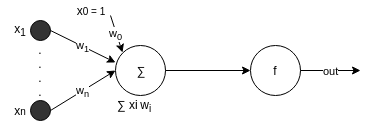
\includegraphics[width=.5\linewidth]{imagenes/perceptron.png}
	\caption{Perceptron con función de activación \textit{f = signo(x)}}
	\label{fig:perceptron}
\end{figure}}

\paragraph{}Cuando se calcula la combinación lineal de los valores de entrada, el valor resultante puede oscilar entre $-\infty$ y $+\infty$, dado que un perceptrón no posee una referencia de cuáles son los límites asociados a las posibles clases de clasificación para el problema de interés.
Las funciones de activación se utilizan con el propósito de limitar este valor al producir la salida del perceptrón. 

\paragraph{}El perceptrón puede ser utilizado para modelar funciones lógicas, como AND, OR, NAND y NOR, ajustando la cantidad de entradas según la cantidad de entradas de la función lógica y ajustando los pesos de tal manera que las salidas sean $1$ y $-1$.
La capacidad de los perceptrones para representar funciones lógicas es relevante puesto que da lugar a que cualquier función lógica pueda ser representada mediante una red de perceptrones de dos niveles de profundidad, en la cual las entradas son conectadas a múltiples perceptrones y las salidas de estos son conectadas a la siguiente capa.
De todas maneras, múltiples capas de perceptrones, dada su naturaleza de unidades lineales, producirán funciones lineales.
Para expresar decisiones no lineales es necesario emplear neuronas cuyas salidas sean funciones no lineales de sus entradas.
Una posibilidad es la utilización de unidades sigmoide, cuya estructura es similar a la del perceptrón, variando en la función de activación, que es la función \textit{sigmoide}, una función no lineal diferenciable.
La personalización de las neuronas artificiales, por lo tanto, genera la posibilidad de representar una gran variedad de funciones.

\paragraph{}Por lo tanto, la forma de trabajar utilizando redes neuronales puede dividirse en dos fases.
Primero, se debe encontrar una configuración arquitectónica de perceptrones o neuronas capaz de expresar la función que se está intentando aprender (que puede no ser conocida a priori y, por lo tanto, puede ser necesario evaluar diversas disposiciones en términos de cantidad de capas y cantidad de neuronas).
Luego, se debe encontrar un vector de pesos $(w_0,w_1,\dots,w_n)$ apropiado para cada perceptrón mediante el entrenamiento. 
En el contexto de un problema de clasificación, entrenar una red neuronal consiste en administrarle ejemplos ya clasificados del problema de interés.
Para cada ejemplo administrado, la red primero producirá una clasificación para el problema dado y la comparará con la salida esperada, tras lo cual ajustará los pesos de cada una de sus unidades para reducir la eventual diferencia entre estos dos valores, utilizando un algoritmo definido previamente.
En este trabajo, donde se utilizan redes multicapa, se utiliza el algoritmo \textit{Backpropagation} para \textit{aprender} los vectores de pesos de cada una de las unidades interconectadas que las componen. 

% TODO hacer notar a renzo inconsistencia en correcciones
\paragraph{}Para describir el funcionamiento del algoritmo Backpropagation, y cómo este ajusta de manera iterativa los pesos de las unidades, es importante definir el concepto de \textit{gradiente descendente}.
Gradiente descendente es una técnica que busca encontrar un mínimo de una función, ya sea local o no. 
Para encontrar un mínimo local de una función usando gradiente descendente, se calcula el gradiente de la misma en un punto de partida y se lo hace variar en dirección negativa a dicho gradiente.
De esta manera, se llegará a un mínimo local eventualmente.
En el contexto de las redes neuronales, la búsqueda por gradiente descendente encuentra un vector de pesos que minimiza el error con respecto al hiperplano generado por los vectores de pesos asociados al conjunto de entrenamiento.
La búsqueda comienza utilizando un vector de pesos inicial arbitrario, modificándolo en pequeños pasos, realizando cada modificación de tal manera que se produzca una disminución en el error con respecto al hiperplano de pesos asociados a la solución.
Este proceso continúa hasta que se llega a un error global mínimo.
Gradiente descendente es una estrategia de búsqueda en un espacio grande o infinito de hipótesis que se puede aplicar siempre que dicho espacio contenga hipótesis que puedan ser determinadas de forma paramétrica, como son los pesos en las unidades.
Así también, se requiere que el error pueda ser diferenciado con respecto a estos parámetros.
Esta estrategia tiene algunas dificultades fundamentales; una de ellas es que la velocidad de convergencia a un mínimo es lenta, pudiendo requerir varios miles de pasos para lograrla y además, si existen varios mínimos locales en la superficie de error, no garantiza que la búsqueda converja a un mínimo global.

\paragraph{}El algoritmo Backpropagation es un método utilizado en redes multicapa para calcular el gradiente que se utiliza para el cálculo de los pesos de las neuronas, empleando gradiente descendente.
El error es calculado en la salida de la red multicapa y es distribuido \textit{hacia atrás}, hacia las capas internas de la red, calculando para cada unidad perteneciente a una capa intermedia su error y actualizando sus pesos.
El bucle de actualización de pesos en Backpropagation puede iterar miles de veces en una aplicación típica de redes neuronales, por lo que existen una variedad de criterios de terminación, como detener el bucle luego de una cantidad fija de iteraciones, o detener el bucle luego de que el error alcanza cierto umbral definido, o por criterios definidos sobre un conjunto dado de prueba. 
Los criterios de terminación son importantes y su elección es delicada dado que, de terminar antes de lo necesario con las iteraciones, la red neuronal puede devolver salidas con un error elevado.
Por otra parte, si se realizan muchas iteraciones se puede generar un sobreajuste de la red neuronal al conjunto de entrenamiento, produciendo resultados de bajo error para el conjunto de entrenamiento, pero con más altos niveles de error para conjuntos de validación con datos no vistos durante el entrenamiento.
Backpropagation no asegura la convergencia a un mínimo global debido al uso gradiente descendente en espacios de hipótesis de alta dimensionalidad (pudiendo haber tantas dimensiones como pesos).
La alta dimensionalidad incrementa la probabilidad de que los movimientos en la superficie de error no permitan alcanzar un mínimo global, pudiendo alcanzar mínimos para una o más dimensiones, que no sean necesariamente mínimos para las otras dimensiones.
A pesar de la falta de garantías con respecto a la convergencia del algoritmo a un mínimo global, Backpropagation es un método de aproximación de funciones altamente efectivo.
Una característica que manifiestan las redes neuronales entrenadas con Backpropagation es la habilidad de descubrir relaciones no triviales presentes en los datos de entrada, a nivel de las capas intermedias ocultas de la red.
Por ejemplo, dada una instancia de entrenamiento con $N$ atributos, la utilización de Backpropagation puede conducir a que se descubran relaciones entre los atributos $a_i$ y $a_j$,  $\forall i, j \in \{1, \dots, N\}, i \neq j$ no identificables por un humano a simple vista, y que contribuyen a la clasificación en gran medida.

\paragraph{}En este trabajo se construyen varios tipos de redes que varían en las funciones de activación utilizadas por las unidades.
A continuación se presentan las funciones de activación que se usaron durante este trabajo. 
La función \textit{tanh}, expresada de la siguiente manera: $f(x) = tanh(x) = \frac{2}{1 + e^{-2x}} - 1 $, es una función continua no lineal.
Al componerla consigo misma se obtienen funciones no lineales, lo que permite combinar a unidades con esta función de activación sin perder la no linealidad. 
tanh es una función suave en su curva, mostrando que pequeñas variaciones en valores del dominio cercanos a 0 generan cambios grandes en los valores correspondientes del codominio.
Esto implica que se le da una gran ponderación a los valores de los extremos del codominio, algo análogo a una tasa de aprendizaje. 

La función \textit{relu}, expresada de la siguiente manera: $f(x) = relu(x) = max(0, x)$ es no lineal y las composiciones de ella consigo misma son no lineales, pero por su forma, puede ocasionar que algunas neuronas den como resultado cero, constituyéndose una eventual pérdida de información.
Este problema se llama \textit{dying relu problem}.
Sin embargo, computar relu es menos costoso que computar tanh porque implica operaciones matemáticas más simples.
Por último, la función \textit{identity}, también llamada de activación lineal, expresada de la siguiente manera: $f(x) = identity(x) = x$, siempre retorna el mismo valor que recibe en su argumento, lo que implica que equivale a una regresión lineal utilizando los pesos de la unidad.

% Ventajas y desventajas
\paragraph{}Entre las ventajas de utilizar redes neuronales se encuentra el hecho de que se adecuan correctamente a problemas en los cuales los datos de entrenamiento contienen ruido y a contextos en los cuales tiempos largos de entrenamiento son aceptables.
Además, las redes neuronales suelen mantener tiempos bajos de clasificación.
Adicionalmente, como se menciona en la Sección \ref{section-trabajos-tecnicas-clasificacion}, una desventaja de las redes neuronales es que su representación interna es difícil de entender para los humanos y, por este motivo, se dice que se comportan como una “caja negra”.

\subsection{SVM}

\paragraph{}Una SVM o máquina de soporte vectorial es un algoritmo o clasificador de aprendizaje automático supervisado utilizado fundamentalmente para problemas de clasificación.
Dado un problema de aprendizaje automático supervisado de clasificación donde las instancias del problema pueden ser clasificadas en $N$ clases y un conjunto de ejemplos de entrenamiento de dicho problema, una SVM busca encontrar un hiperplano que los divida de manera lineal esas $N$ clases. De esta manera, frente a una nueva instancia del problema, la SVM será capaz de clasificarla generando una correspondencia entre esta instancia y una de las $N$ clases posibles.

\paragraph{}Se denominan vectores de soporte a aquellos ejemplos de entrenamiento más cercanos al hiperplano, la distancia entre el hiperplano y un vector de soporte se conoce como margen y para un conjunto de ejemplos de entrenamiento, SVM busca dividirlos de manera óptima con un hiperplano donde se maximice estos márgenes para cada uno de los vectores de soporte, cada uno asociado a su vez a una de las posibles clases de clasificación del problema. En un problema donde las instancias pueden ser clasificadas en dos clases, el hiperplano de dos dimensiones es representado por una línea recta y los vectores de soporte son aquellos ejemplos de entrenamiento más cercanos a ella, desde las dos direcciones posibles. La figura \ref{fig:svm_margin} muestra lo antedicho.

\textsc{\begin{figure}[ht!]
	\centering
    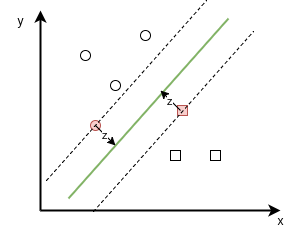
\includegraphics[width=.5\linewidth]{imagenes/svm_margenes.png}
	\caption{En esta figura se observan dos conjuntos de elementos (cuadrados y círculos), clasificados en dos clases, en base a dos características, \textit{x} e \textit{y}. El hiperplano generado por svm se muestra como la recta negra y se marcan los márgenes en lineas punteadas. Así, en color rojo se muestran los vectores de soporte, uno perteneciente a cada clase, siendo z la distancia entre cada vector de soporte y el hiperplano.}
	\label{fig:svm_margin}
\end{figure}}


\paragraph{}El hiperplano estará dado por la ecuación $g(\vec{x}) = \vec{w}^T\vec{x} + w_0$ donde $\vec{w}$ es un vector de pesos y $\vec{x}$ es el vector de características. La distancia a uno de los márgenes está dada por $z = \abs{g(\vec{x})} / \norm{\vec{w}} = 1 / \norm{\vec{w}}$, por lo que el margen total se computa como $1 / \norm{\vec{w}} +  1 / \norm{\vec{w}} = 2 / \norm{\vec{w}}$. Por lo tanto, minimizando la expresión $\norm{\vec{w}}$ se maximizan los márgenes, maximizando la separabilidad de las clases. La confianza en la clasificación de una instancia del problema estará dada por la distancia de dicha instancia al hiperplano de manera directamente proporcional.

\paragraph{}Cuando se tienen más de dos clases objetivo para la clasificación, se utiliza un SVM multiclase en el cual la técnica de aprendizaje admite dos posibles estrategias. Por un lado \textit{One vs. Rest} (\textit{OVR}) y por otro \textit{One vs. One} (\textit{OVO}). Dado un conjunto de $N$ clases $\{c_1,c_2,\dots,c_N\}$, \textit{OVR} intentará clasificar $c_i$ contra $\{c_1,c_2,\dots,c_{i-1},c_{i+1},\dots,c_{N - 1}\}$ dejando como representantes de la clase $C_N$ los datos que no fueron clasificado en las otras clases. Por otro lado \textit{OVO}, intentará clasificar cada clase $i$ contra cada $C_j \forall j \neq i$, creando un hiperplano para cada una de las combinaciones. Comparando las dos estrategias, \textit{OVR} genera $C_{N-1}$ clasificadores, en contraste con \textit{OVO} que generará una combinación de $N$ tomada de a dos, generando un número mayor de clasificadores que \textit{OVR}. Por otro lado, \textit{OVR} es más sensible al no balance de los datos, en el sentido de que si intento clasificar  y la cantidad de datos representantes de esta clase es baja en comparación con el total de datos, esta clase podría verse eclipsada por las demás. En cambio, con \textit{OVO} este fenómeno no se manifiesta en igual medida, dado que se generan clasificadores uno a uno. La figura \ref{fig:ovoovr} muestra lo antedicho.

\textsc{\begin{figure}[ht!]
	\centering
    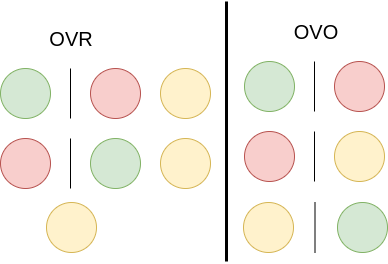
\includegraphics[width=.5\linewidth]{imagenes/ovoovr.png}
	\caption{A la izquierda se muestra la estrategia de entrenamiento de SVM \textit{OVR}, en la cual cada una de las clases se intenta clasificar contra el resto de las clases. A la derecha se muestra la estrategia \textit{OVO}, que genera clasificadores para cada par de clases.}
	\label{fig:ovoovr}
\end{figure}}

\paragraph{}La obtención de un hiperplano que divida de manera lineal a los ejemplos de entrenamiento no siempre es posible. Cuando no es posible, se suele utilizar una técnica conocida como \textit{kernelización} o \textit{Kernel Trick} para aumentar la dimensión del dominio donde se está buscando un hiperplano e intentar obtener un hiperplano que separe linealmente a los ejemplos de entrenamiento en esa dimensión. De esta manera, es posible clasificar a nuevas instancias del problema de acuerdo a este nuevo hiperplano y transformar la clasificación obtenida a la dimensión original del problema dada por las clases de clasificación disponibles. De todas maneras, una utilización imprudente del \textit{Kernel Trick} puede llevar a un sobreajuste del modelo.

\paragraph{}Entre las desventajas de utilizar SVM encontramos que los tiempos de entrenamiento asociados pueden ser significativos para grandes conjuntos de entrenamiento, pudiendo tener consumos considerables de memoria tanto en entrenamiento como en pruebas. Así también la selección de parámetros de \textit{Kernel} para el realizar el \textit{Kernel Trick} puede ser complejo y se debe ejecutar evitando el sobreajuste.


  \chapter{Trabajos relacionados} \label{section-trabajo-relacionado}
\markright{Trabajos relacionados}

\paragraph{}En este capítulo se describen los principales trabajos relacionados a la temática abordada en este proyecto.
El paradigma SV ha sido explorado únicamente en dos trabajos \cite{savant-original} \cite{savant-bag}, que son abordados en la Sección \ref{section-trabajos-relacionados-savant}.
La Sección \ref{section-trabajos-tecnicas-clasificacion} está dedicada a técnicas de clasificación en aprendizaje supervisado, mientras que la Sección \ref{section-trabajos-seleccion-extraccion-atributos} trata la temática de selección y extracción de atributos en aprendizaje automático.
Finalmente, en la Sección \ref{section-trabajos-relacionados-mapreduce} se aborda el modelo de programación MapReduce, que permite la ejecución paralela en un sistema implementado bajo el paradigma SV.

% ############### RESEÑA ###############

\section{Savant Virtual} \label{section-trabajos-relacionados-savant}

% FIRST
% citep para que aparezca algo tipo Dorronsoro et al [1]
% cite o citet para que aparezca sólo la referencia del estilo [1]
\paragraph{} El síndrome de Savant es una condición donde los individuos que la padecen, conocidos como savants, son capaces de resolver tareas de cálculo, memoria o mnemotecnia, como encontrar el día de la semana para una fecha dada o listar números primos utilizando \textit{métodos desconocidos}, en tiempos inferiores a los esperados normalmente y con una gran precisión. 

\paragraph{}Tomando como inspiración al síndrome de Savant, \citet{savant-original} introdujeron el paradigma SV con el objetivo de generar programas que, utilizando aprendizaje automático supervisado, encuentren soluciones a problemas con una calidad comparable a las soluciones ofrecidas por otros algoritmos conocidos.
De esta manera, el componente de aprendizaje automático está asociado de manera simbólica a las reglas que un Savant incorpora automáticamente.
Los autores aplicaron el paradigma SV sobre el problema HCSP, presentado en la Sección \ref{section-descripcion-problema}, utilizando también a Min-Min como criterio de referencia para llevar a cabo el aprendizaje automático.
Con el objetivo de aplicar SV a la resolución de este problema de manera paralela, el sistema planteado implementó el modelo MapReduce.
Bajo este modelo, cada \textit{mapper} se corresponde con un clasificador multiclase entrenado previamente (utilizando SVM). Un único \textit{reducer} realiza una búsqueda local con el objetivo de mejorar la solución y posteriormente devuelve su solución.
El sistema permite utilizar tantos \textit{mappers} como tareas se tengan en la instancia del problema, posibilitando la ejecución en paralelo de cada uno.
Por otra parte, cada clasificador del sistema se entrena utilizando las soluciones obtenidas mediante la aplicación del algoritmo Min-Min.
Finalmente, se consigue un sistema que puede trabajar de manera paralela, generando soluciones basadas en un entrenamiento realizado utilizando el criterio Min-Min como referencia. 

Los autores evaluaron el paradigma propuesto sobre un conjunto de instancias de prueba generadas de forma aleatoria (en la forma de matrices ETC, como fue presentado en la Sección \ref{section:descripcion-problema,subsection:estimacion-tiempo-ejecucion}), con el objetivo de comparar las soluciones obtenidas mediante Savant con las de Min-Min.
Cada instancia de prueba estaba compuesta por un conjunto de tareas, un conjunto de máquinas y las duraciones de las tareas para cada máquina. 
% TODO tal vez dar un poco más de detalle del estudio, tipo decir cuántas instancias se usaron
Los resultados mostraron una precisión promedio (similitud con la solución de referencia) del 82\%, resultando mejor la precisión para instancias más pequeñas del problema (128 tareas y 4 máquinas) que para instancias de mayor tamaño (512 tareas y 16 máquinas). 
% TODO ¿poner dimensiones como $128 \times 4$ ya que esta notación es explicada en la parte de descripción del problema?
Fueron obtenidos mejores resultados al utilizar un \textit{reducer} con búsqueda local frente a un \textit{reducer} simple que genera una solución en base a la salida directa de cada \textit{mapper} sin hacer modificaciones.
En algunas instancias de prueba SV fue capaz de encontrar mejores soluciones que Min-Min. 

El trabajo de \citet{savant-original} presenta oportunidades de trabajo futuro desde diversos puntos de vista; el \textit{reducer} puede llevar a cabo una búsqueda paralela de mejores soluciones, se puede estudiar el uso de otro tipo de clasificadores y se pueden estudiar aplicaciones para verificar la adaptabilidad de SV a otros problemas y comparar su desempeño frente al obtenido para el problema HCSP. 

Este trabajo representó el punto de partida para la investigación en torno a SV y proporciona el marco de trabajo que se sigue en el proyecto de grado, dado que involucra el mismo modelo conceptual, tipos de pruebas y modelado de problemas.

% SECOND
\paragraph{}En \citet{savant-bag} se estudió la aplicación de SV para la generación automática de programas para resolver el problema de la mochila.
Evaluar SV para el problema de la mochila resulta interesante porque representa un problema de optimización combinatoria NP-difícil y además es un tipo de problema diferente al estudiado en el trabajo previo (HCSP) en términos de sus variables binarias y con restricciones simples, en vez de enteras y sin restricciones.
En este problema se tiene un contenedor con una capacidad $W$ y un conjunto $E$ de $n$ objetos, cada uno con un beneficio $p_i$ y un peso $w_i$ que no excede a $W$.
El objetivo perseguido al resolver este problema es el de seleccionar objetos de $E$ a introducir en el contenedor, maximizando el beneficio que estos aportan, sujeto a que la suma de los pesos de los objetos introducidos no exceda la capacidad $W$.
Con respecto al modelado del problema, se optó por representar a una instancia con un peso asociado a la capacidad del contenedor estudiado y un vector donde cada índice representa a un objeto con su peso y su beneficio asociado.
Se aplicó SV respetando el modelo planteado en \citet{savant-original}, utilizando también SVM como clasificador y mapper.
En particular, se utilizaron tantos \textit{mappers} (replicados) como objetos disponibles en la instancia del problema y la clasificación de cada \textit{mapper} indicaba si ese objeto había sido incluido o no en la selección de objetos asignados al contenedor.
Con respecto al \textit{reducer}, se aplicó una búsqueda local aleatorizada a la hora de generar la solución frente a una instancia del problema y dos mecanismos de corrección para soluciones infactibles: corrección ávida por beneficio y corrección ávida por peso.
La corrección ávida por beneficio se basa en eliminar sucesivamente el objeto que aporte el menor beneficio hasta llegar a una solución factible, mientras que la corrección ávida por peso se basa en buscar al objeto de menor peso que tenga un peso mayor o igual al sobrepeso de la solución y eliminarlo, o eliminar al objeto de mayor peso en caso de no encontrarse objetos que cumplan con la condición anterior.
Durante el trabajo se utilizaron 15.750 instancias del problema (en varios conjuntos de datos), de entre 100 y 1.500 objetos, con correlación de peso y beneficio variable para cada tamaño del problema.
Con el fin de determinar una selección de atributos adecuada (dado que se contaba con información de peso y beneficio para cada objeto y además la capacidad del contenedor), se estudió la precisión media (porcentaje de soluciones correctas retornadas por la SVM) para cada conjunto de datos disponible, utilizando una selección diferente en cada instancia del estudio para el entrenamiento.
Dado que la precisión media para todas las configuraciones fue elevada y hubieron diferencias pequeñas entre las configuraciones con respecto a este valor, se optó por emplear al tipo de selección más sencillo y directo, que resultó ser el peso del objeto, su beneficio y la capacidad de la mochila.
Experimentalmente se determinó que al utilizar más del 15\% de los datos para entrenar al clasificador las mejoras en precisión resultaron marginales, por lo que se optó por utilizar únicamente ese porcentaje de los datos, reduciendo de esta manera los tiempos de entrenamiento de la SVM.
Como resultado se obtuvo un error medio del 3,2\% con respecto al resultado óptimo para cada instancia del problema, obtenido mediante el uso de un algoritmo exacto de referencia.
El valor del trabajo de \citet{savant-bag} para este proyecto de grado reside en el hecho de que amplía la información disponible en relación a SV.

% ############### RESEÑA ###############
\section{Técnicas de clasificación} \label{section-trabajos-tecnicas-clasificacion}

\paragraph{}El trabajo de \citet{ml-survey} presenta una reseña sobre métodos de aprendizaje automático, principalmente de carácter expositivo, que ofrece guías acerca de cómo seleccionar apropiadamente clasificadores de aprendizaje automático para casos de uso comúnmente encontrados en la práctica.
Se presenta a los árboles de decisión, que ofrecen buenos resultados para problemas donde los atributos toman valores discretos o categóricos; por lo tanto no sería acertado aplicarlos para un problema de optimización combinatoria con variables numéricas, como es el caso del problema estudiado en este proyecto de grado.
Se destaca el hecho de que los algoritmos estadísticos en general resultan menos precisos que aquellos más sofisticados como las redes neuronales artificiales, aunque tienen tiempos de aprendizaje menores.
Los algoritmos como las redes neuronales artificiales o SVM requieren de un mayor ajuste de parámetros, no son modelos interpretables por humanos y requieren de un gran conjunto de datos de entrenamiento para ser precisos al clasificar.
Por otra parte, se presentan algoritmos lógicos como el de \textit{k-nearest neighbors} o \textit{KNN}, que tienen parámetros sencillos de ajustar y son transparentes en términos de su funcionamiento, pero que involucran una carga de memoria poco conveniente a la hora de estudiar problemas de grandes dimensiones.

\newpage % orphaned line.

El valor del trabajo de \citet{ml-survey} para este proyecto de grado reside en la guía comparativa de selección de métodos de aprendizaje automático que ofrece, que presenta los algoritmos más comunes para cada variante de aprendizaje automático, como \textit{ID3} para árboles de decisión y \textit{Backpropagation} para redes neuronales.

% ############### RESEÑA ###############

\section{Selección y extracción de atributos} \label{section-trabajos-seleccion-extraccion-atributos}

\paragraph{} El trabajo de \citet{fs-survey} ofrece información acerca de las técnicas más utilizadas para la selección de atributos en aprendizaje automático.
La selección de atributos refiere a la acción de seleccionar un subconjunto de atributos o \textit{features} de las instancias del problema a resolver, que efectivamente puedan describir al problema reduciendo el efecto del ruido o variables irrelevantes.
Además, al reducir la cantidad de variables que describen un problema es posible comprender los datos de mejor manera y reducir los requerimientos computacionales asociados a su manejo.
El problema de seleccionar atributos resulta no trivial dado que si las instancias de entrenamiento utilizadas tienen $N$ atributos posibles, es necesario tomar en cuenta $2^N$ subconjuntos posibles de atributos. \citet{fs-survey} presentan los siguientes tipos de métodos de selección de atributos para aprendizaje supervisado:
\begin{itemize}
\item \textit{Filter}: Ordena a los atributos de acuerdo a algún criterio de ordenamiento que les asigna un valor y elimina aquellos atributos que queden por debajo de un umbral mínimo.
Se sugieren algoritmos para la determinación de la relevancia de cada atributo, siendo el algoritmo \textit{Mutual Information} el más relevante, que mediante el cálculo de la entropía condicional entre dos atributos determina qué tan dependientes son entre sí, lo que permite determinar qué tan dependiente es un atributo de la clasificación de una instancia de entrenamiento.
\item \textit{Wrapper}: Se utilizan algoritmos de búsqueda para encontrar un subconjunto de atributos de manera heurística, no exacta.
Cada subconjunto se evalúa construyendo un clasificador entrenado con los datos sesgados utilizando únicamente los atributos del subconjunto de atributos obtenido y evaluando su precisión con respecto a un conjunto de validación.
Este tipo de método de selección resulta muy costoso en términos computacionales, especialmente si el conjunto de datos es muy extenso.
\item \textit{Embedded}: Este tipo de métodos surgió como respuesta a los problemas de eficiencia asociados a los métodos de tipo \textit{Wrapper}.
Utilizan una alternativa para la evaluación, dada por una función objetivo basada en la entropía condicional entre los atributos del subconjunto de atributos actual y la clasificación.
Este tipo de método de selección reduce el tiempo computacional requerido por métodos de tipo \textit{Wrapper}.
\end{itemize}
\paragraph{}A pesar de que cada algoritmo de selección de atributos puede comportarse de manera diferente de acuerdo al tipo de datos utilizado, \citet{fs-survey} llevaron a cabo un experimento para mostrar la diferencia entre utilizar selección de atributos y no hacerlo.
En dicho experimento se generaron conjuntos de datos, cada uno correspondiente a una condición médica, teniendo potencialmente distintos atributos.
Cada instancia de entrenamiento constaba de entradas asociadas a señales eléctricas provenientes de un sistema médico y una salida o clasificación que indicaba a qué condición médica correspondían esas entradas (cáncer, diabetes, etc.).
Para cada conjunto de datos se destinó el 50\% al entrenamiento y el 50\% a la validación y se consideró como medida de rendimiento la precisión de cada clasificador sobre el conjunto de validación.
Se encontró que, en general, la precisión de los clasificadores que usaban selección de atributos (reduciendo la cantidad de atributos a la mitad) se mantenía muy próxima a la de los clasificadores que utilizaban todos los atributos.
Por ejemplo, para un conjunto de datos que determinaba si un paciente tenía cáncer de acuerdo a 10 atributos, un clasificador (en particular SVM) obtuvo una precisión mayor al 96\%, mientras que el mismo clasificador entrenado con 5 atributos mantuvo una precisión del 95\%.
Este trabajo resultó de gran importancia para determinar cómo llevar a cabo la selección de atributos para la representación del problema estudiado en este proyecto de grado.

% SECOND
\paragraph{}El trabajo de \citet{survey-feature-selection-extraction} analiza un conjunto de técnicas para la selección y extracción de atributos, con el propósito de determinar qué tan efectivas son estas técnicas a la hora de lograr un alto desempeño en clasificación.
Se presentan métodos de selección de atributos como mecanismos para la obtención de conjuntos de datos de menor dimensión.
Los métodos de selección de atributos pueden ser caracterizados por las siguientes etapas: búsquedas sobre los datos, generación de subconjuntos de datos y medida de la mejora en el subconjunto de datos.
Por otro lado, la extracción de atributos se presenta como la generación de nuevas características para reducir la complejidad y dar una representación más simple de los datos, expresando cada variable en el espacio de características nuevas como una combinación lineal de las variables originales.
Experimentalmente, se estudiaron siete conjuntos de datos médicos que incluían información sobre enfermedades oncológicas.
Los resultados obtenidos mostraron que el uso de técnicas de extracción de características permite obtener una mejor precisión que el uso de selección de características.
En particular, se ubicó a PCA (\textit{Principal Component Analysis}) como el método de extracción de características más utilizado.
PCA es un método no paramétrico simple que consiste en una transformación lineal de los datos que minimiza la redundancia, medida como la covarianza, maximizando la información, medida como la varianza.
Este método tiene las siguientes limitaciones: asume que la relación entre las variables es lineal, su interpretación de los datos resulta razonable únicamente si se asume que todas las variables están escaladas numéricamente y carece de un modelo probabilístico.
Para sobrellevar las dos primeras limitaciones se propuso el método PCA no lineal, donde las variables son observadas como categóricas.
Para afrontar la última limitación se propuso el método PPCA (\textit{Probabilistic Principal Component Analysis}), en el que PCA es uno de los parámetros de un modelo probabilístico. 
El trabajo de \citet{survey-feature-selection-extraction} fue un gran aporte a la hora de determinar cómo llevar a cabo la selección y/o extracción de atributos para la representación del problema estudiado en este proyecto de grado.

% ############### RESEÑA ###############

\section{MapReduce} \label{section-trabajos-relacionados-mapreduce}

\paragraph{}En el trabajo de \citet{mapreduce} se presenta una introducción al modelo MapReduce, así como detalles de su implementación y de su rendimiento.
Mapreduce es un modelo de programación utilizado para procesar y generar grandes conjuntos de datos.
En términos genéricos, un sistema implementado bajo el modelo MapReduce recibe datos en forma de un conjunto de pares (clave, valor), los transforma mediante la aplicación de una función definida por el usuario y devuelve un conjunto de pares (clave, valor) de salida agregados de acuerdo a un criterio también definido por el usuario.
La transformación aplicada a los datos en la entrada del sistema se llama \textit{map} y la transformación aplicada a los datos en la salida del sistema se llama \textit{reduce}.
En la implementación propuesta por los autores, la computación dada en las funciones \textit{map} y \textit{reduce} es paralelizada automáticamente en múltiples recursos de cómputo, posibilitando el procesamiento masivo y paralelo de datos.
En concreto, el sistema presentado se encarga de inicializar múltiples hilos de ejecución en un régimen maestro-esclavo, donde el hilo maestro se encarga de asignar tareas \textit{map} o \textit{reduce} a los hilos esclavos.
De esta manera, se cuenta con \textit{map workers} y \textit{reduce workers}.
Cada \textit{map worker} recibe una porción de los datos, los procesa y guarda su salida en un disco local.
Cada \textit{reduce worker} recibe una ubicación (como por ejemplo una referencia a otra máquina de la red en un cluster) de donde deberá leer los datos intermedios generados por los \textit{map workers}, procesarlos y guardar su salida en un archivo.
Cuando todos los hilos finalizan su ejecución, el hilo \textit{master} retoma el control y reanuda la ejecución del programa de usuario que haya desencadenado la ejecución del MapReduce.
En el trabajo de \citet{mapreduce} también se mencionan técnicas utilizadas para el control de fallas, balanceo de carga y detalles específicos de implementación.
Además, se muestra una serie de resultados experimentales que consisten en una evaluación del rendimiento del modelo ejecutado en un cluster de 1800 máquinas de iguales características, en dos tipos de computación: búsqueda de un patrón en un terabyte de datos y ordenamiento de un terabyte de datos. 
El valor de este trabajo en relación al proyecto de grado reside en el hecho de que SV propone generar programas concurrentes automáticamente y la utilización de MapReduce puede resultar útil para posibilitar el paralelismo en dichos programas.

\section{Resumen}

\paragraph{}La Tabla \ref{table:trabajos-relacionados} presenta un resumen de los trabajos relacionados, manteniendo el orden en el que fueron mencionados en las secciones previas.
Se indica el autor, el año de publicación del trabajo y una breve descripción con los conceptos clave del mismo.

% ############### TABLA ###############
\begin{table}[htb]
\centering
\begin{tabular}{P{0.25\linewidth} P{0.05\linewidth} P{0.55\linewidth} } 
\specialrule{.2em}{.1em}{.1em} 
\multicolumn{1}{c}{Autores} & \multicolumn{1}{c}{Año}  & \multicolumn{1}{c}{Conceptos clave}\\ 
\hline
\citet{savant-original} & 2013 & Se presenta el paradigma Savant para la paralelización de una heurística de planificación con aprendizaje automático utilizando SVM \\ 
\hline
\citet{savant-bag} & 2016 & Estudio del problema de la mochila bajo el paradigma Savant \\
\hline
\citet{ml-survey} & 2007 & Compendio de las técnicas de clasificación más utilizadas en aprendizaje automático supervisado \\
\hline
\citet{fs-survey} & 2014 & Estudio comparativo de técnicas de selección de atributos en aprendizaje automático \\
\hline
\citet{survey-feature-selection-extraction} & 2014 & Compendio de técnicas de selección de atributos en aprendizaje automático, con foco en PCA \\
\hline
\citet{mapreduce} & 2008 & Utilización de MapReduce para procesamiento de grandes volúmenes de datos en clusters \\
\specialrule{.2em}{.1em}{.1em} 
\end{tabular}
\caption{Trabajos relacionados al proyecto de grado}
\label{table:trabajos-relacionados}
\end{table}
% ############### FIN TABLA ###############

\paragraph{} El análisis de la literatura relacionada muestra que el paradigma SV en particular no ha sido estudiado de manera extensiva y permite llegar a la conclusión de que existe lugar para contribuir, por ejemplo profundizando en la utilización de métodos de aprendizaje automático distintos a SVM.

\newpage
  \chapter{Implementación} \label{chapter-implementation}
\markright{Implementación}

\paragraph{} En este capítulo se presenta el sistema de software construido para evaluar el rendimiento comparativo de las redes neuronales y SVM en términos del aprendizaje del problema HCSP.
Este sistema fue implementado utilizando \textit{Python} y la biblioteca de aprendizaje automático \textit{Scikit-learn}, entre otras.

\paragraph{} La arquitectura del sistema está conformada por tres componentes fundamentales.
El primero es el módulo encargado de generar los datos utilizados en forma de ejemplos de entrenamiento.
Este módulo se describe en la sección \ref{chapter-implementacion:data}.
También se tiene un módulo dedicado a la generación de clasificadores, incluyendo redes neuronales y SVM.
Este módulo se describe en la sección \ref{chapter-implementacion:clasificadores}.
Finalmente, descrito en la sección \ref{chapter-implementacion:clasificacion}, se tiene un módulo encargado de clasificar nuevas instancias del problema.

% TODO agregar diagrama arquitectónico o algo.

\section{Generación de instancias del problema e instancias de entrenamiento} \label{chapter-implementacion:data}

\paragraph{} Dado el problema HCSP, surgen dos posibles maneras de utilizar una instancia del problema (dado por una matriz ETC) y su resolución (una planificación) en el contexto de aprendizaje automático.
Una opción implica utilizar a la matriz ETC completa como entrada del clasificador de elección y, hacer que la salida esperada sea la planificación, es decir todas las asignaciones tarea-máquina esperadas.
Esto constituye un problema de clasificación multiclase, y la desventaja principal que presenta es la de no permitir escalar en términos de máquinas o tareas.
Esto implica que si un clasificador es entrenado para aprender a resolver el problema HCSP con instancias del problema de dimensión $M \times N$, no será aplicable para ninguna otra dimensión.
La otra opción que se presenta, y la que fue escogida finalmente en este trabajo tomando como referencia el trabajo de \citet{savant-original}, es la de descomponer a una matriz ETC en varios ejemplos de entrenamiento.
Por lo tanto, dado un ejemplo de entrenamiento bajo este paradigma, se tiene a la información asociada únicamente a una tarea como la entrada, y a la asignación tarea-máquina de esa tarea como la salida esperada.
Esto causa que una instancia del problema (con su planificación asociada) de dimensión $M \times N$ se convierta en $M$ potenciales ejemplos de entrenamiento, y proporciona la posibilidad de escalar en términos de la cantidad de tareas a ejecutar.
Esta oportunidad surge dado el hecho de que ahora un ejemplo de entrenamiento está limitado únicamente por la cantidad de máquinas, y se presenta con más detalle en la sección \ref{chapter-implementacion:clasificadores}.
% matriz entera
% matriz parcial


\paragraph{} Con el objetivo de generar ejemplos de entrenamiento y validación como los discutidos anteriormente para entrenar y evaluar a los clasificadores construidos, fue necesario desarrollar un componente de software que pudiera hacerlo a demanda.
Este componente está conformado fundamentalmente por scripts, y en la Figura \ref{fig:diagrama-datos} se puede ver un diagrama de secuencia donde se explicita su funcionamiento. 

\paragraph{} Inicialmente, se utiliza un script extraído de \citet{bib-doctorado-nesmachnow} para generar instancias del problema, y se genera una solución para dicha instancia utilizando una implementación de Min-Min.
% TODO tal vez agregar implementación en apéndice.
Estos elementos son persistidos directamente al sistema de archivos de manera iterativa, de acuerdo a la cantidad de ejemplos de entrenamiento que se deseen generar.
Una vez finalizada esta etapa, es necesario modificar la estructura de los datos generados, de manera de obtener aquella estructura soportada por los clasificadores de aprendizaje automático.
Por lo tanto, se procede a tomar cada par constituido por una instancia del problema y su planificación esperada, y se generan tantos ejemplos de entrenamiento como tareas existan en la instancia del problema.
Es decir que para una instancia del problema de dimensión $M \times N$ tendremos $M$ ejemplos de entrenamiento.
Finalmente, se agrupan estos ejemplos de entrenamiento y se persisten en formato CSV para su uso posterior.
Este formato es utilizado por ser el estándar soportado más comúnmente por las librerías de manejo de datos utilizadas.

\textsc{\begin{figure}[ht!]
	\centering
    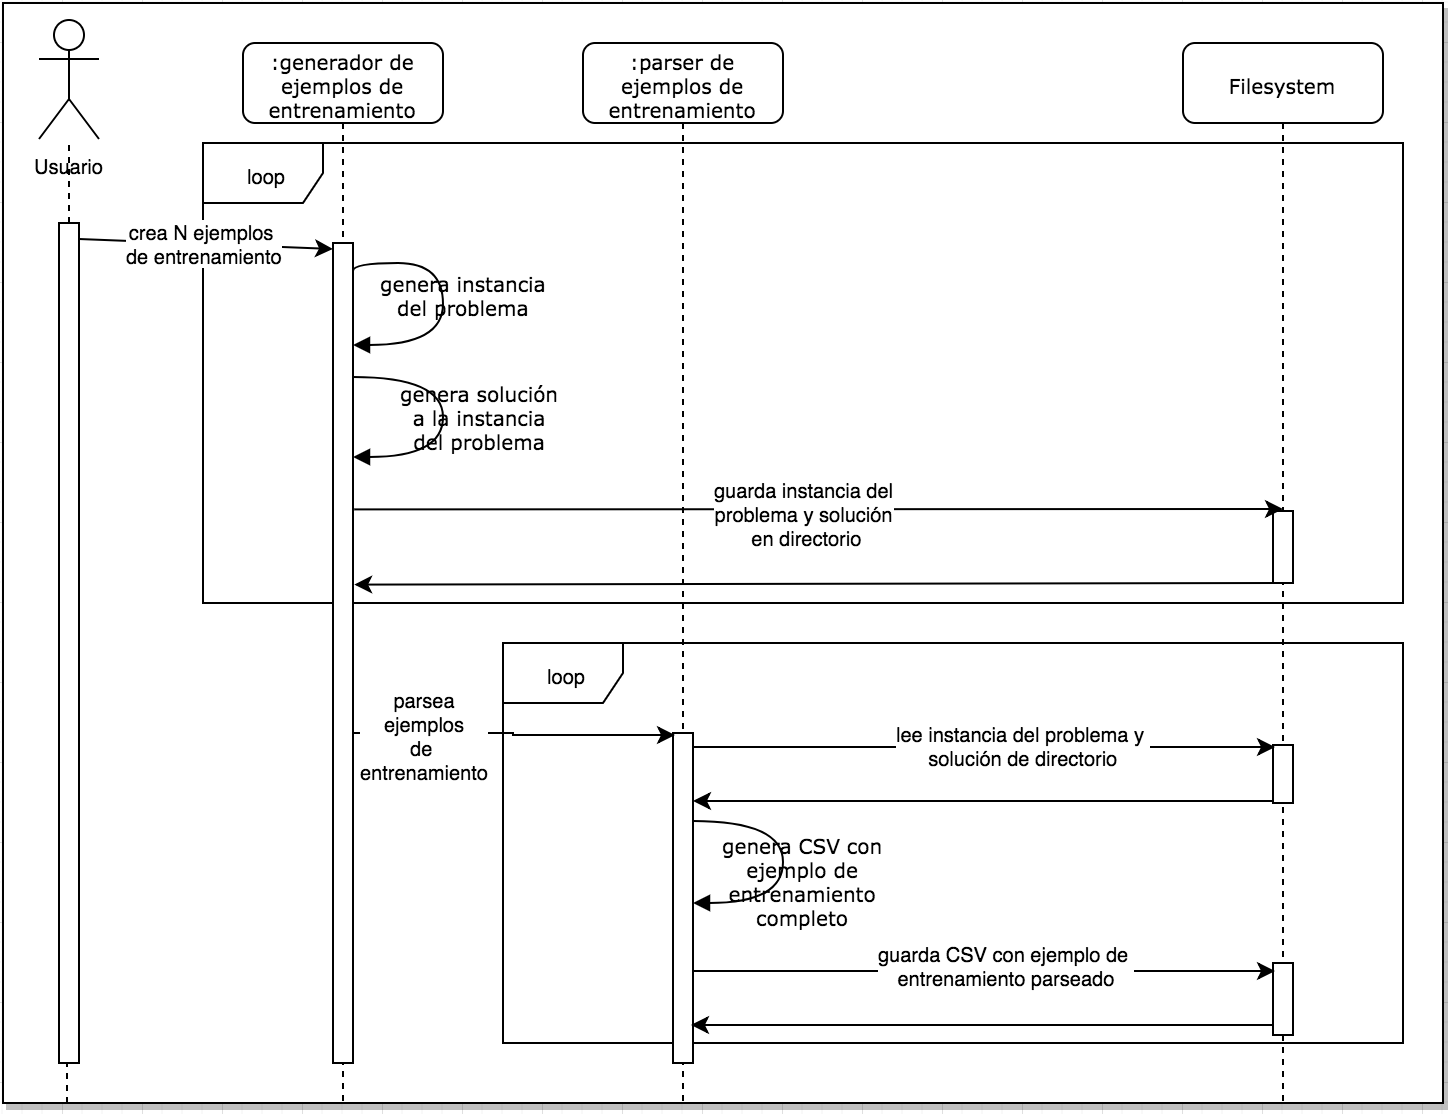
\includegraphics[width=.9\linewidth]{imagenes/implementacion/diagrama-datos.png}
	\caption{Diagrama de secuencia de generación de ejemplos de entrenamiento.}
	\label{fig:diagrama-datos}
\end{figure}}

\paragraph{} Este componente de software, como el resto de los aquí mencionados, fue desarrollado de manera de permitir su ejecución automatizada, a pesar de existir un usuario presente en el diagrama de secuencia.
Dicho usuario puede bien ser un usuario final o un script encargado de invocar a este sistema.
La posibilidad de automatización favorece la generación de ejemplos de entrenamiento a gran escala y de manera paralela mediante el uso de hilos.
Además, se ofrece al usuario la posibilidad de determinar cuántas instancias del problema (con sus correspondientes soluciones) serán generadas, dónde se persisten, y las características de los tipos de instancias del problema a generar, como por ejemplo la dimensión de las mismas.

\section{Generación de clasificadores y entrenamiento} \label{chapter-implementacion:clasificadores}

\paragraph{} Se implementó un componente de software dedicado a crear, entrenar y persistir clasificadores de aprendizaje automático. Este componente permite seleccionar como clasificador de aprendizaje automático a utilizar \textit{SVM} o redes neuronales.

\paragraph{} Se utiliza la librería \textit{Pandas}\cite{bib-pandas} de \textit{Python}. Esta librería simplifica el manejo de datos mediante estructuras de datos indizadas, proporcionando un conjunto de métodos que permiten realizar operaciones sobre éstas estructuras para facilitar el análisis de los datos, haciendo un uso eficiente de los recursos computacionales sobre los que se ejecute.

\paragraph{} Como se mencionó en la sección \ref{chapter-implementacion:data}, se utilizó cada fila de la matriz ETC del problema como los atributos para un único ejemplo de entrenamiento. Esto quiere decir que para una matriz de $512$ tareas y $16$ máquinas, se obtendrán $512$ ejemplos de entrenamiento, cada uno clasificado en una de las $16$ clases objetivo. Estas clases corresponden una a una con las máquinas asignadas por el algoritmo $Min-Min$. La figura \ref{table:datosentrenamiento} muestra un ejemplo de matriz ETC de $512$ tareas y $16$ máquinas, cada tarea con su máquina asignada siendo esta asignación la clasificación del ejemplo de entrenamiento.


\begin{figure}[ht!]
\[
\begin{bmatrix}
     & m_1 & m_2 & \dots  & m_{16} & objetivo \\
    t_1 & 35.74 & 39.62 & \dots  & 456.89 & 4 \\
    t_2 & 75.55 & 97.41a & \dots  & 579.19 & 3 \\
    \vdots & \vdots & \vdots & \vdots & \vdots & \vdots\\
    t_{512} & 130.12 & 216.59 & \dots  & 789.84 & 5\\
\end{bmatrix}
\]
\caption{Ejemplo de matriz ETC con atributo objetivo para el aprendizaje. Cada $t_i$ con $i = 1 \dots 512$ es información correspondiente a una tarea. La columna objetivo muestra la asignación de máquina para la correspondiente tarea $i$ y éste es el atributo objetivo para los clasificadores. La información asociada a la tarea, que incluye los tiempos de ejecución estimados de la tarea $t_i$ para cada una de las máquinas disponibles, junto con su clasificación, equivale a un ejemplo de entrenamiento para el clasificador.}
\label{table:datosentrenamiento}
\end{figure}

\paragraph{}A diferencia de utilizar la matriz ETC completa como ejemplo de entrenamiento, utilizar cada fila de la matriz se traduce en menores tiempos de entrenamiento y además da flexibilidad a la hora de clasificar problemas con otro número de tareas e igual número de máquinas. Esto es, como los clasificadores se entrenan con información referente a cada tarea, se pueden clasificar problemas que tengan número menor o mayor de tareas. Este tipo de escalado en función de tareas es además realista, ya que en la práctica el hardware tiende a ser una restricción menos flexible que la cantidad de tareas, algo que puede fluctuar con mayor frecuencia en función del tiempo dependiendo del caso de estudio.

\paragraph{} Para el entrenamiento se utilizaron $100$ instancias del problema de dimensión $512 \times 16$, lo que se traduce en $51200$ instancias de entrenamiento, cada una con un atributo objetivo que varía entre $1$ a $16$, siendo este el identificador de la máquina la cual la tarea es asignada. El componente de software implementado carga en memoria 100 archivos $csv$ que se encuentran en un directorio definido. Cada uno de estos archivos es una matriz ETC con el atributo objetivo correspondiente asignado para cada tarea, como se muestra en la figura \ref{table:datosentrenamiento}. Estos atributos objetivo se agregan en un sólo \textit{DataFrame}\cite{DataFrame-pandas} de \textit{Pandas}. Este \textit{DataFrame} es escalado y utilizado para el entrenamiento de los clasificadores.

\paragraph{} Debido a que los datos contienen atributos cuyas magnitudes tienen una gran varianza y los algoritmos utilizados manejan distancias euclideanas para el aprendizaje, los datos fueron escalados antes de realizarse el entrenamiento de los clasificadores. Otra razón para esclar los datos antes del entrenamiento es que \textit{Gradiente Descendente} tiende a converger más rápido cuando los datos están escalados\cite{gradiente-descendente-escalado}.

\paragraph{} El escalado de los datos se realiza mediante la clase $preprocessing.StandardScaler()$ de la librería \textit{Scikit-Learn} para \textit{Python} \cite{scikit-learn}. Esta librería provee el soporte para los métodos de aprendizaje automático y herramientas para el preprocesamiento de los datos. En particular la clase $StandardScaler()$ analiza cada atributo de manera independiente y almacena la mediana y la desviación estándar para luego ser utilizados en datos nuevos que ingresan al modelo \cite{StandardScaler-scikit-learn}.

\paragraph{} Para la construcción de los clasificadores de aprendizaje automático se utilizaron las clases \textit{svm.SVC} para la construcción de \textit{SVM} y \textit{neural\_network.MLPClassifier} para la construcción de las redes neuronales, ambas clases pertenecientes a la librería \textit{Scikit-Learn} de \textit{Python}.

\paragraph{} Con respecto al clasificador \textit{SVM}, el mismo se utilizó siguiendo la estrategia \textit{OVR}, dado que genera menos clasificadores que mediante la estrategia \textit{OVO} de acuerdo a lo expuesto en la sección \ref{capitulo:svm}. Además, se entendió \textit{OVR} como la mejor estrategia dada la baja heterogeneidad de las instancias del problema, por lo cual se espera no tener un desbalance en la cantidad de representantes de cada clase.

\paragraph{} Con respecto a las redes neuronales, en particular sobre la arquitectura de las mismas, se siguió la heurística recomendada por \citet{bib-heuristic-hobs}, dada la falta de consenso existente en la comunidad con respecto a la manera óptima de determinar la cantidad de neuronas en las capas ocultas de una red neuronal de acuerdo a los casos de uso en los que se apliquen dichos clasificadores. Según esta heurística, la cantidad de neuronas en una capa oculta (o $N_h$) se determina con la siguiente fórmula $N_h = \frac{N_s} {(\alpha * (N_i + N_o))}$, siendo:
\\
\\
$N_i$ = cantidad de neuronas de entrada
\\
\\
$N_o$ = cantidad de neuronas de salida
\\
\\
$N_s$ = cantidad de instancias de entrenamiento
\\
\\
$\alpha$ = factor de escalamiento arbitrario, con valor igual a 2 para este estudio

\paragraph{} El resto de los parámetros iniciales de configuración de la red neuronal se definieron utilizando la clase \textit{model\_selection.GridSearchCV}, que realiza una búsqueda exhaustiva de los mejores parámetros para el modelo mediante validación cruzada. A medida que se avanzó con el trabajo, estos parámetros fueron modificados para ajustarlos a las necesidades puntuales del proyecto. El detalle de los parámetros iniciales selectos se encuentra en la sección \ref{capitulo:configuracion}.
% TODO ¿agregar info sobre el clasificador usado para redes neuronales (MLPClassifier)?

% TODO la ref Pipeline-scikit-learn no figura en bibliography.bib
\paragraph{} A un nivel de abstracción superior, tanto para SVM como para redes neuronales, se utilizó la clase \textit{pipeline.Pipeline}\cite{Pipeline-scikit-learn} de la librería \textit{Scikit-Learn}. Esta clase envuelve al clasificador escogido, y permite que los datos fluyan desde su forma original, pasando secuencialmente por cada etapa del preprocesamiento, para finalmente ingresar en el clasificador. Esto permite la evaluación del modelo con estrategias como valización cruzada, simplificando la implementación del preprocesamiento de los datos mediante una encadenación de transformaciones atómicas. En particular, se utilizó un \textit{Pipeline} con el escalado encadenado al clasificador seleccionado. 

\paragraph{} Finalmente, el componente de software desarrollado se encarga de persistir los clasificadores generados. Para esto se utiliza la clase \textit{externals.Joblib} de \textit{Scikit-Learn}. El uso de \textit{Joblib} es sugerido cuando se utilizan clasificadores de \textit{Scikit-Learn}, dado que provee una manera eficiente de almacenar objetos que contienen gran cantidad de \textit{arrays} de \textit{numpy}\cite{numpy}, que es el caso de modelos de \textit{Scikit-Learn} ya entrenados.\cite{persistence}. Esta librería no solo permite la persistencia de los modelos sino que también permite la carga de los mismos en memoria para su utilización.



\newpage % orphaned line.

\section{Clasificación} \label{chapter-implementacion:clasificacion}

\paragraph{} En lo que respecta a la clasificación, se implementó un componente encargado de clasificar un conjunto de ejemplos de validación dado uno o más clasificadores ya entrenados.
Llevar a cabo esta implementación fue necesario dado que por restricciones de los recursos disponibles, evaluar el rendimiento de los clasificadores construidos mediante validación cruzada insumía una gran cantidad tiempo, limitando la agilidad del desarrollo.
Como consecuencia, se consideró como alternativa válida separar un conjunto de datos de validación a clasificar con este módulo, con el fin de obtener métricas de rendimiento de esta manera. 

\paragraph{} El componente implementado, además de disponibilizar las funcionalidades descritas anteriormente, proporciona métricas de interés adicionales.
Dentro de las métricas calculadas se encuentran el makespan esperado y el obtenido mediante predicciones.
Estas métricas son consideradas como fundamentales para evaluar el rendimiento de los clasificadores, dado que de manera independiente a la precisión, es necesario evaluar la métrica fundamental asociada al éxito de una solución del problema HCSP, que como se explica en la Sección \ref{section:descripcion-problema,subsection:estimacion-tiempo-ejecucion}, es el tiempo insumido por la máquina que finaliza su ejecución por último.
Con estos dos valores se puede evaluar qué tan exitosa fue la planificación obtenida mediante el uso de clasificadores en comparación con la solución obtenida mediante la heurística de referencia.
Finalmente, se calcula el porcentaje de ocasiones en las que el clasificador, al predecir erróneamente, escoge una máquina más rápida (constituyendo una acción ávida).
Esta métrica se calcula con el fin de evaluar si un clasificador se alejó de lo esperado en términos de precisión y makespan por haber aprendido a comportarse de manera ávida y por lo tanto aprendiendo a maximizar el beneficio local para cada tarea.

\paragraph{} La implementación del componente de clasificación consta fundamentalmente de scripts, y la Figura \ref{fig:diagrama-clasificacion} presenta un diagrama de secuencia que explicita su funcionamiento.

\newpage % orphaned line.

\paragraph{} En la implementación, inicialmente se invoca el script encargado de realizar todo este análisis sobre un conjunto de ejemplos de validación.
Estos ejemplos de validación deben estar presentes en un directorio especificado mediante opciones al invocar el script.
Posteriormente, el script invoca al script de clasificación sobre cada uno de los ejemplos de validación encontrados.
El script de clasificación se encarga de cargar el clasificador a utilizar desde una ubicación especificada del sistema de archivos.
Una vez que todas las instancias de validación se encuentran clasificadas, se efectúa el cálculo de métricas en el script de análisis.
Finalmente, el resultado es devuelto al usuario.

\textsc{\begin{figure}[ht!]
	\centering
    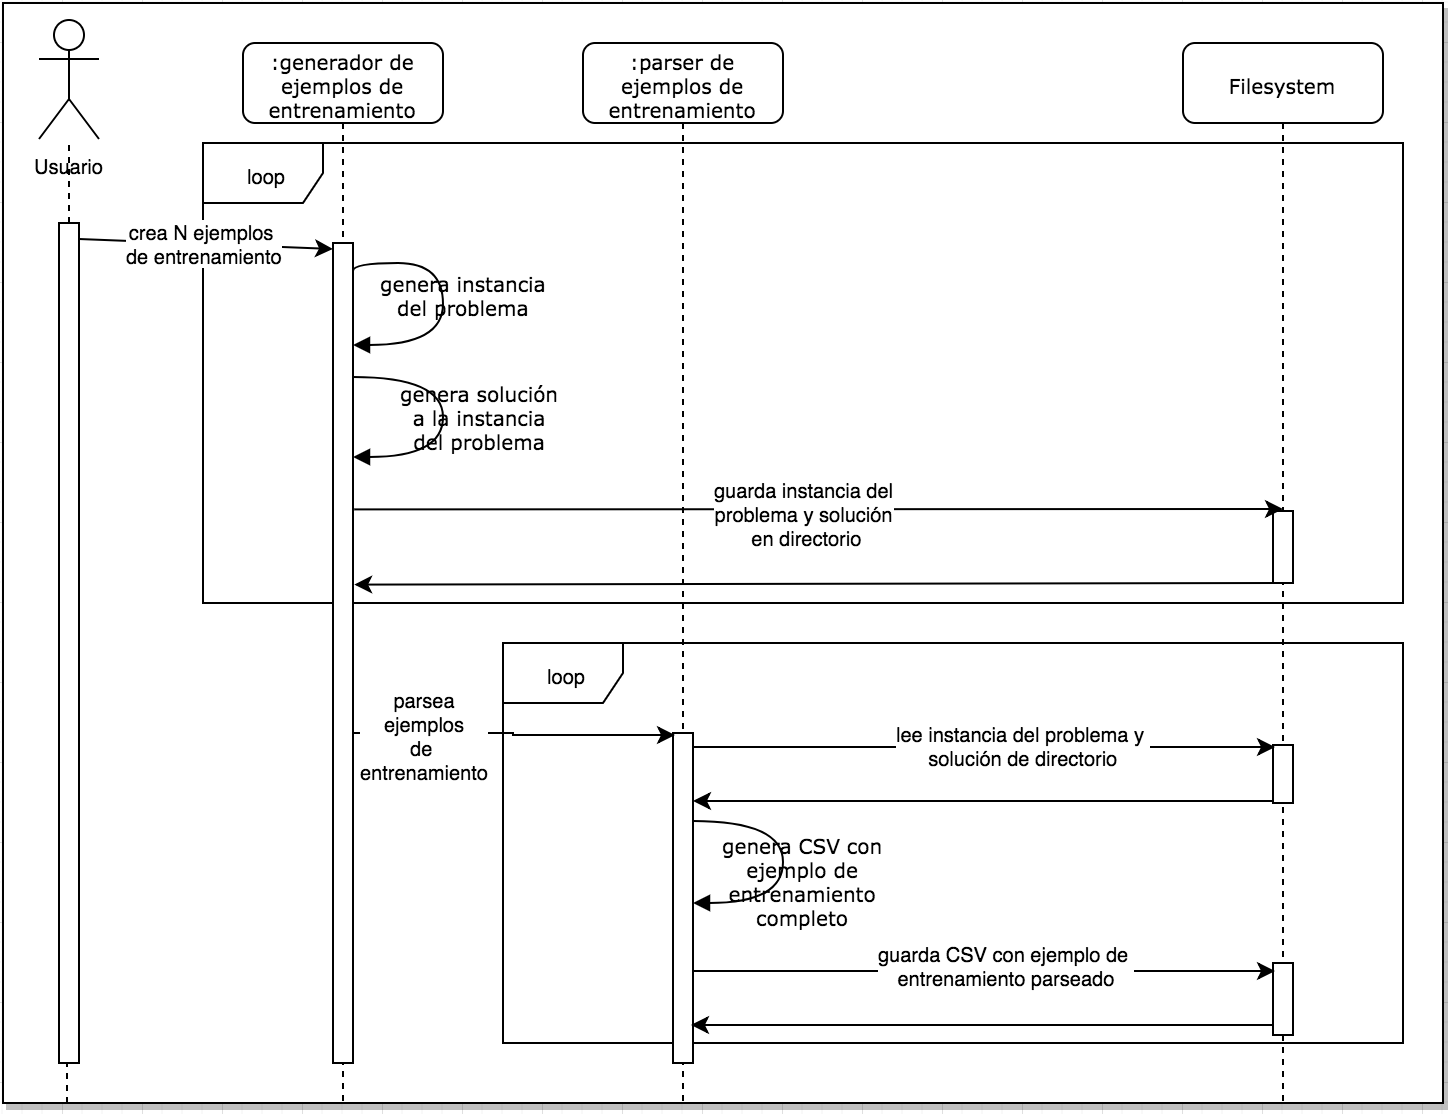
\includegraphics[width=.9\linewidth]{imagenes/implementacion/diagrama-datos.png} % TODO cambiar por validation
	\caption{Diagrama de secuencia de clasificación de ejemplos de validación.}
	\label{fig:diagrama-clasificacion}
\end{figure}}




  \chapter{Análisis Experimental} \label{capitulo:analisis-experimental}
\markright{Análisis Experimental}

En este capítulo se presentan las decisiones tomadas en torno a las configuraciones de los clasificadores y el análisis de los resultados obtenidos durante los experimentos. 

\section{Decisiones de configuración} \label{capitulo:configuracion}

\paragraph{} Durante el análisis experimental fueron realizadas comparaciones entre las clasificaciones obtenidas por redes neuronales y SVM.
En particular, fue de interés estudiar el comportamiento de las redes neuronales y SVM en términos del tamaño del problema.

\paragraph{} Tomando el trabajo de \citet{savant-original} como inspiración, se optó por trabajar con clasificadores entrenados con una determinada dimensión del problema (en particular $512$ tareas sobre $16$ máquinas o $512\times 16$) a la hora de clasificar y evaluar instancias del problema con menor, igual y mayor cantidad de tareas.
Para hacer esto posible, se generaron instancias del problema de dimensión $512\times 16$, utilizadas para el entrenamiento de los clasificadores.
Así también, como se presentó en la Sección \ref{chapter-implementacion:data}, para cada dimensión del problema desde $17\times 16$ hasta $1024\times 16$, se generaron conjuntos de $10$ instancias del problema, las cuales fueron utilizadas para calcular y comparar la precisión en la clasificación para redes neuronales y SVM.

\newpage % orphaned line.

\paragraph{} Las redes neuronales fueron entrenadas con diferentes cantidades de capas ocultas, habiéndose generado con $2$, $3$ y $4$ capas ocultas, siendo 4 el máximo número de capas ocultas empleado debido a limitaciones de recursos y tiempos de entrenamiento altos.

\paragraph{} Como fue mencionado en el Capítulo \ref{chapter-implementation}, para obtener una primera selección de parámetros de configuración para el entrenamiento de las redes neuronales se utilizó el método \textit{GridSearch} de la clase \textit{model\_selection.GridSearchCV} de \textit{scikit-learn}.
Este método realiza una búsqueda, mediante validación cruzada, de los mejores parámetros para el entrenamiento de un clasificador.
Para eso es necesario definir conjuntos de posibles valores a ser utilizados en los parámetros de los clasificadores.
A continuación se presentan los valores considerados para cada uno de esos parámetros.
Para el parámetro  \textit{solver}, se consideraron el método de optimización de los pesos \textit{Broyden–Fletcher–Goldfarb–Shanno} para memoria limitada (\textit{lbfgs}), Gradiente Descendente (\textit{sgd}) y el método Adam (\textit{adam}).
Para el coeficiente de aprendizaje, llamado \textit{alpha}, se consideraron los valores \textit{0.01} y \textit{0.0001}.
Finalmente, para el parámetro \textit{activation}, que indica la función de activación utilizada, se consideraron las funciones \textit{relu}, \textit{tanh} e \textit{identity}.
Los resultados del método \textit{GridSearch} para los parámetros mencionados se muestran en la Tabla \ref{table:parametros}.
Con respecto al parámetro \textit{activation} se observó que el valor seleccionado por el método \textit{GridSearch} fue \textit{relu}; esto fue de particular interés debido a que dicha función de activación cambia de forma abrupta en su pendiente. Las primeras pruebas realizadas utilizando la red neuronal con activación \textit{relu}, brindaron resultados de \textit{makespan} mayores a los resultados de \textit{makespan} generados por SVM. 
Al variar la función de activación de la red neuronal, se obtuvieron resultados de \textit{makespan} menores a los valores de \textit{makespan} obtenidos con SVM.
Esto llevó a variar las funciones de activación para estudiar el comportamiento de las redes neuronales con funciones de activación con pendientes que no tuvieran cambios abruptos.
El resto de los parámetros se mantuvieron de acuerdo a los resultados del método \textit{GridSearch}.

\begin{table}[h!]
\centering
\begin{tabular}{ |p{0.25\linewidth}|p{0.25\linewidth}| } 
\hline
\textbf{Parámetro} & \textbf{Valor}\\
\hline
solver & lbfgs\\ 
\hline
alpha & 0.01\\ 
\hline
activation & relu\\ 
\hline
\end{tabular}
\caption{ Valores para los parámetros de las redes neuronales, obtenidos mediante el método \textit{GridSearch} de la biblioteca \textit{scikit-learn}}
\label{table:parametros}
\end{table}

\paragraph{} Se evaluaron las redes neuronales resultantes de las combinaciones de las funciones de activación \textit{relu}, \textit{tanh} e \textit{identity} y las cantidades de capas ocultas, profundizando en las pruebas para aquellas combinaciones que mostraban resultados más prometedores.

\section{Análisis combinado para redes neuronales de 2, 3 y 4 capas ocultas}

\paragraph{}En primer lugar fueron comparados los resultados de \textit{makespan} para soluciones obtenidas a partir de las redes neuronales, utilizando como funciones de activación a \textit{tanh}, \textit{identity} y \textit{relu}, con 2, 3 y 4 capas ocultas.
Asimismo, en esta comparación, también fueron analizados los resultados obtenidos con SVM. 

\paragraph{} Cada clasificador fue entrenado con 100 instancias del problema de dimensión $512\times16$, lo que se traduce en 51200 instancias de entrenamiento para los clasificadores. Para cada dimensión del rango estudiado, se utilizaron 10 instancias del problema para validar el rendimiento de las redes neuronales y SVM. Los resultados presentados en esta Sección son promedios de los resultados individuales de estas 10 instancias.

\paragraph{} Fueron identificados aquellos clasificadores que obtuvieron mejores resultados en \textit{makespan}.
Las Figuras \ref{fig:relu234}, \ref{fig:identity234} y \ref{fig:tanh234} muestran las diferencias porcentuales de \textit{makespan} con respecto al \textit{makespan} obtenido por el algoritmo Min-Min, para la clasificación de instancias del problema en un rango de dimensiones que va desde $17\times16$ a $1024\times16$.

\paragraph{} De manera similar, los resultados también fueron agrupados de acuerdo a su dimensión.
Esta agrupación fue realizada de a 200 tareas con la excepción de que el primero y el último de los conjuntos van desde la dimensión $17\times16$ a $200\times16$ y $1000\times16$ a $1024\times16$, respectivamente.

\paragraph{}La Figura \ref{fig:relu234} muestra los resultados para las redes neuronales utilizando la función de activación \textit{relu}.
En dicha figura se observa que el \textit{makespan} obtenido por los resultados de la SVM se aproxima más al \textit{makespan} dado por los resultados del algoritmo Min-Min que para los resultados obtenidos con las redes neuronales, cualquiera sea la cantidad de capas ocultas utilizada. 

\paragraph{} Cabe destacar que a medida que aumenta la cantidad de capas ocultas de la red neuronal, los resultados se alejan de los valores esperados llegando, para clasificaciones sobre dimensiones pequeñas, a estar a más del $100\%$ por sobre los valores esperados.
Los mejores resultados de las redes neuronales se observan para aquellas redes neuronales con solo dos capas ocultas.
% TODO ¿agregar algo sobre que probablemente la función aprendida no requiere de la complejidad que permite una mayor cantidad de capas ocultas? 


\begin{figure}[H]
  \centering
  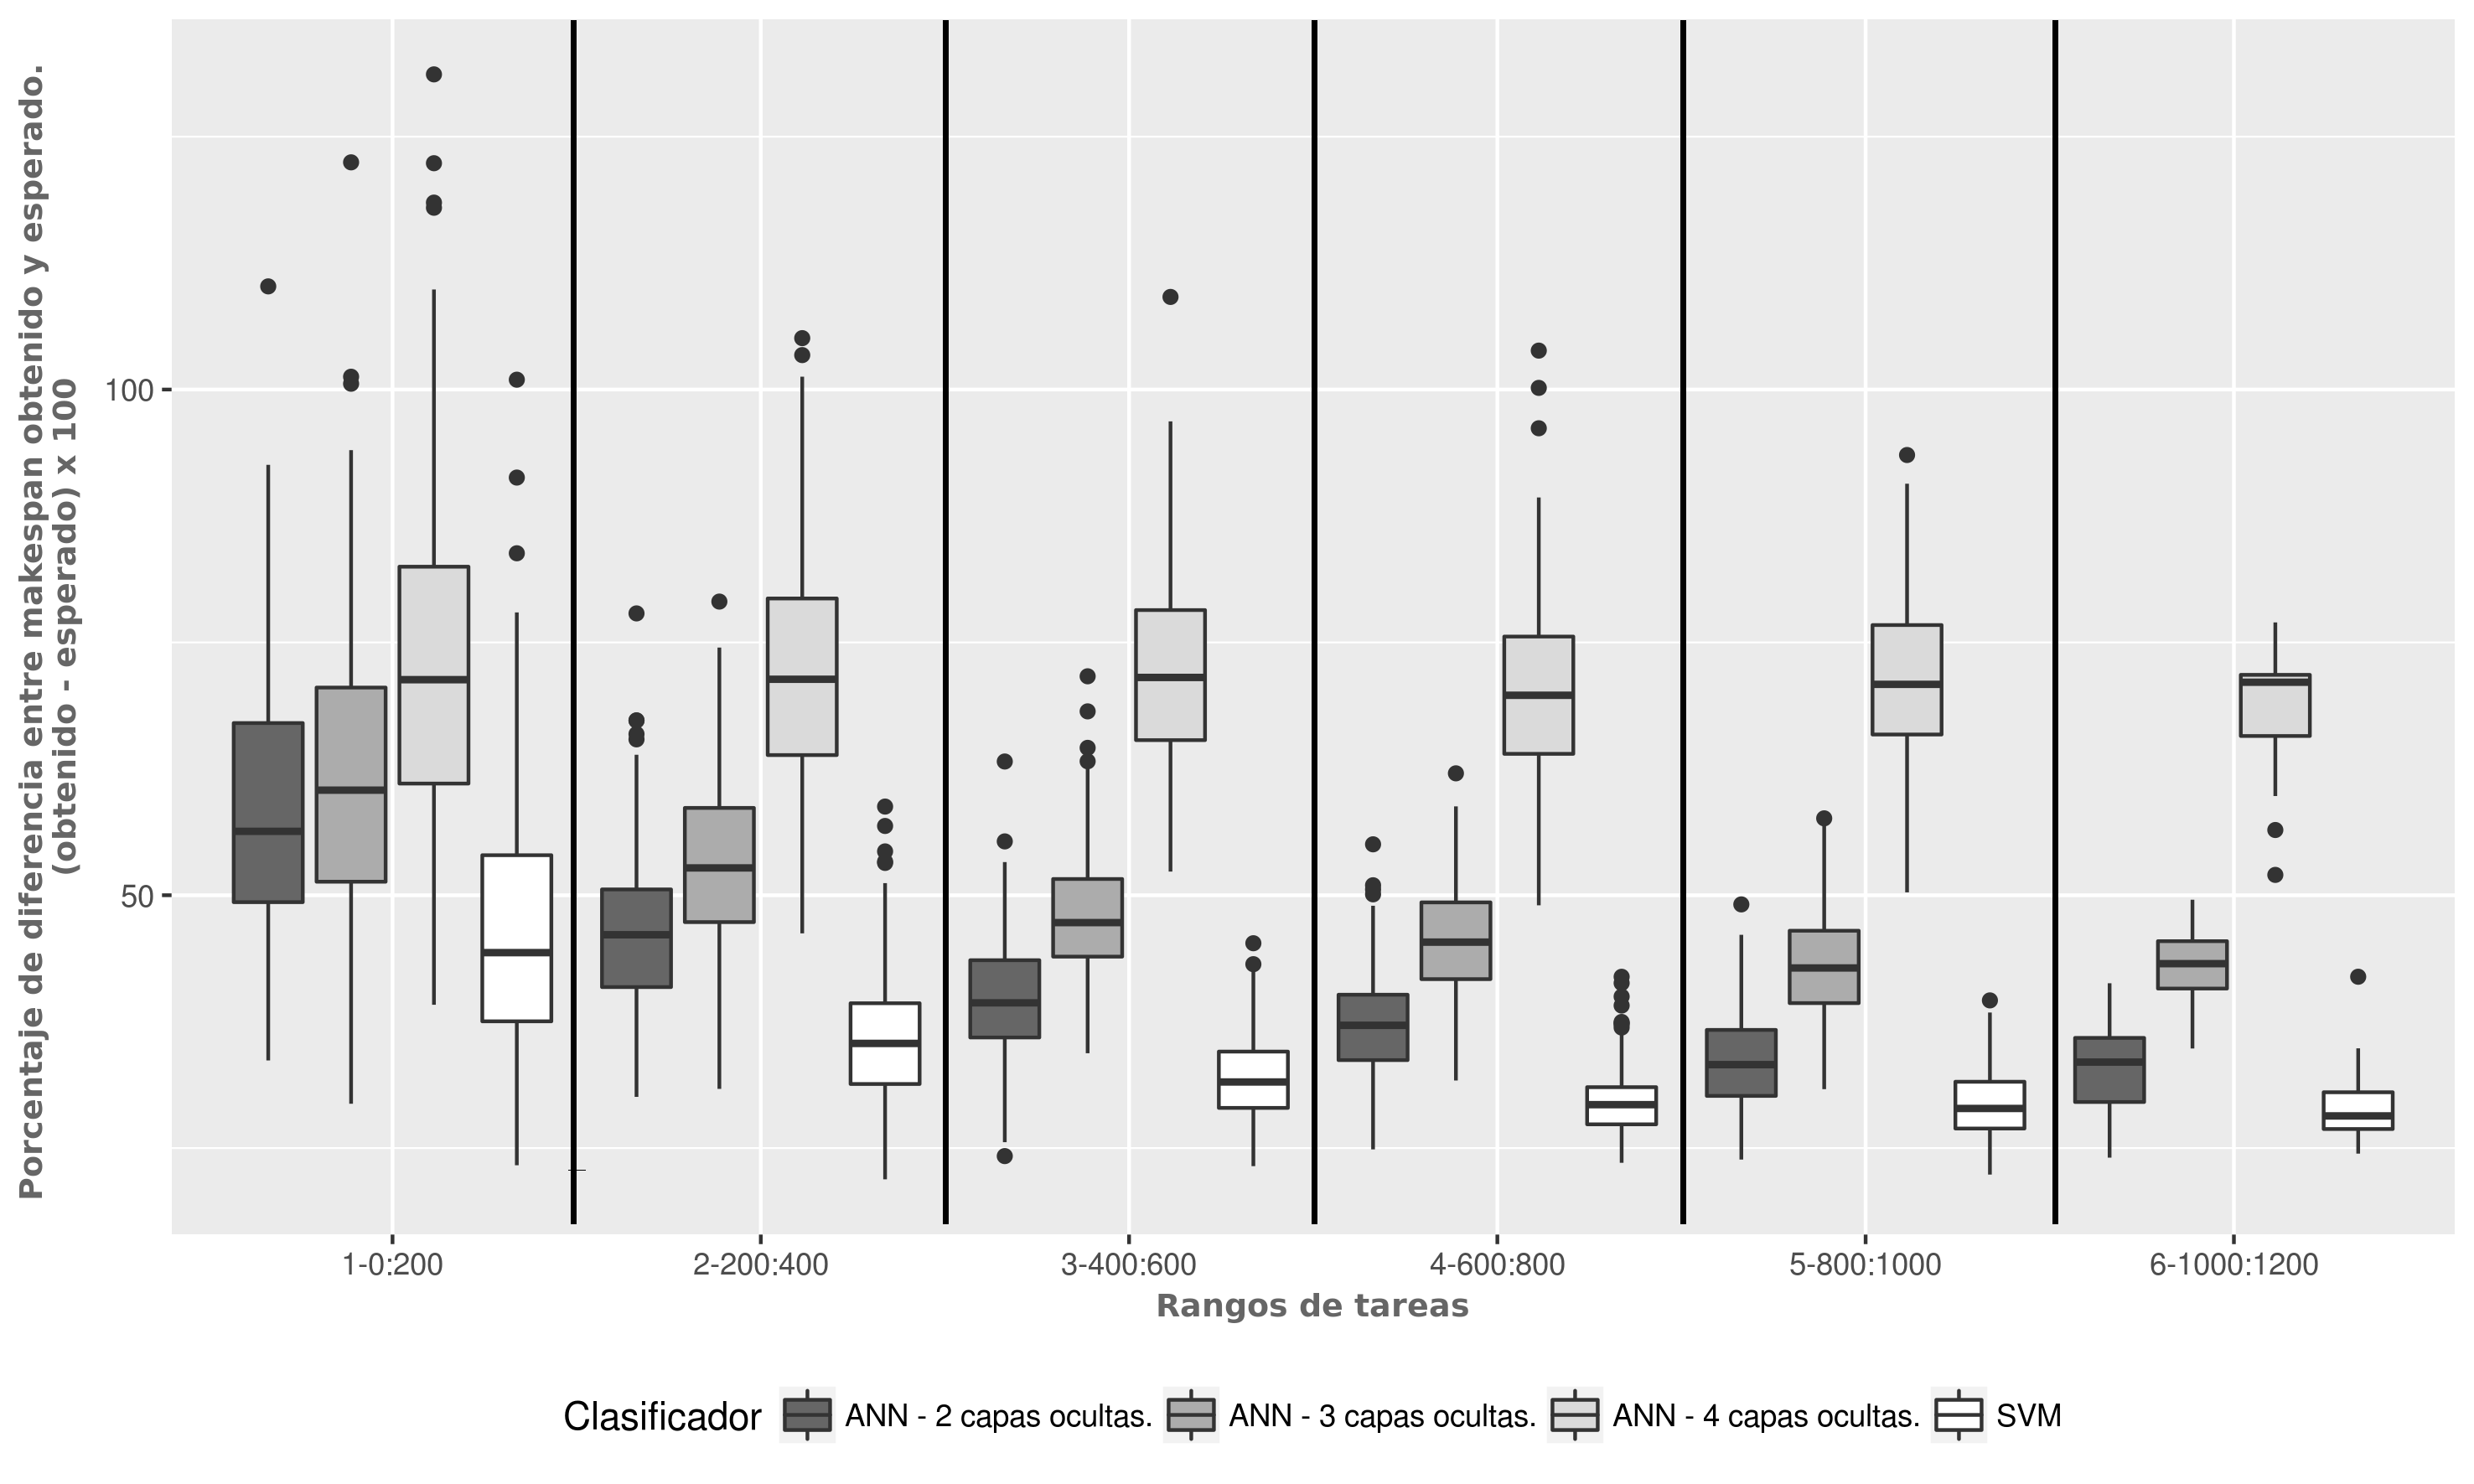
\includegraphics[width=\columnwidth]{imagenes/comparacion_anns_relu_2.png}
  \caption{Comparación de  la diferencia porcentual  de los resultados de \textit{makespan} para redes neuronales con función de activación \textit{relu} y para SVM, con respecto al \textit{makespan} obtenido por el algoritmo Min-Min.
Se comparan redes neuronales de 2, 3 y 4 capas ocultas.}
  \label{fig:relu234}
\end{figure}

\paragraph{}La Figura \ref{fig:identity234} muestra los resultados para las redes neuronales utilizando la función de activación \textit{identity}.
En este caso los resultados para las redes neuronales son más próximos a los valores esperados dados por el algoritmo Min-Min que los resultados dados por SVM.
Ya desde tareas de dimensión $ 200 \times 16$ se comienzan a observar mejoras en el \textit{makespan}, siendo aún más evidentes para instancias del problema de dimensión mayor.
Nuevamente se observa que los resultados más próximos al \textit{makespan} esperado están dados por la red neuronal con dos capas ocultas. 

\newpage % orphaned line.

\paragraph{}En la Figura \ref{fig:tanh234} se observan los resultados para las redes neuronales utilizando la función de activación \textit{tanh}.
En este caso, la red neuronal con dos capas ocultas mejora los resultados obtenidos a partir de instancias del problema de dimensión $ 400 \times 16$ en adelante. 

\paragraph{} En los casos presentados en las Figuras \ref{fig:relu234}, \ref{fig:identity234} y \ref{fig:tanh234}, los mejores resultados de las redes neuronales se encontraron para aquellas de solo dos capas ocultas. Fue profundizado el estudio de las redes neuronales con solo dos capas ocultas, de cara a entender mejor la naturaleza de las soluciones generadas. 

\textsc{\begin{figure}[H]
  \centering
  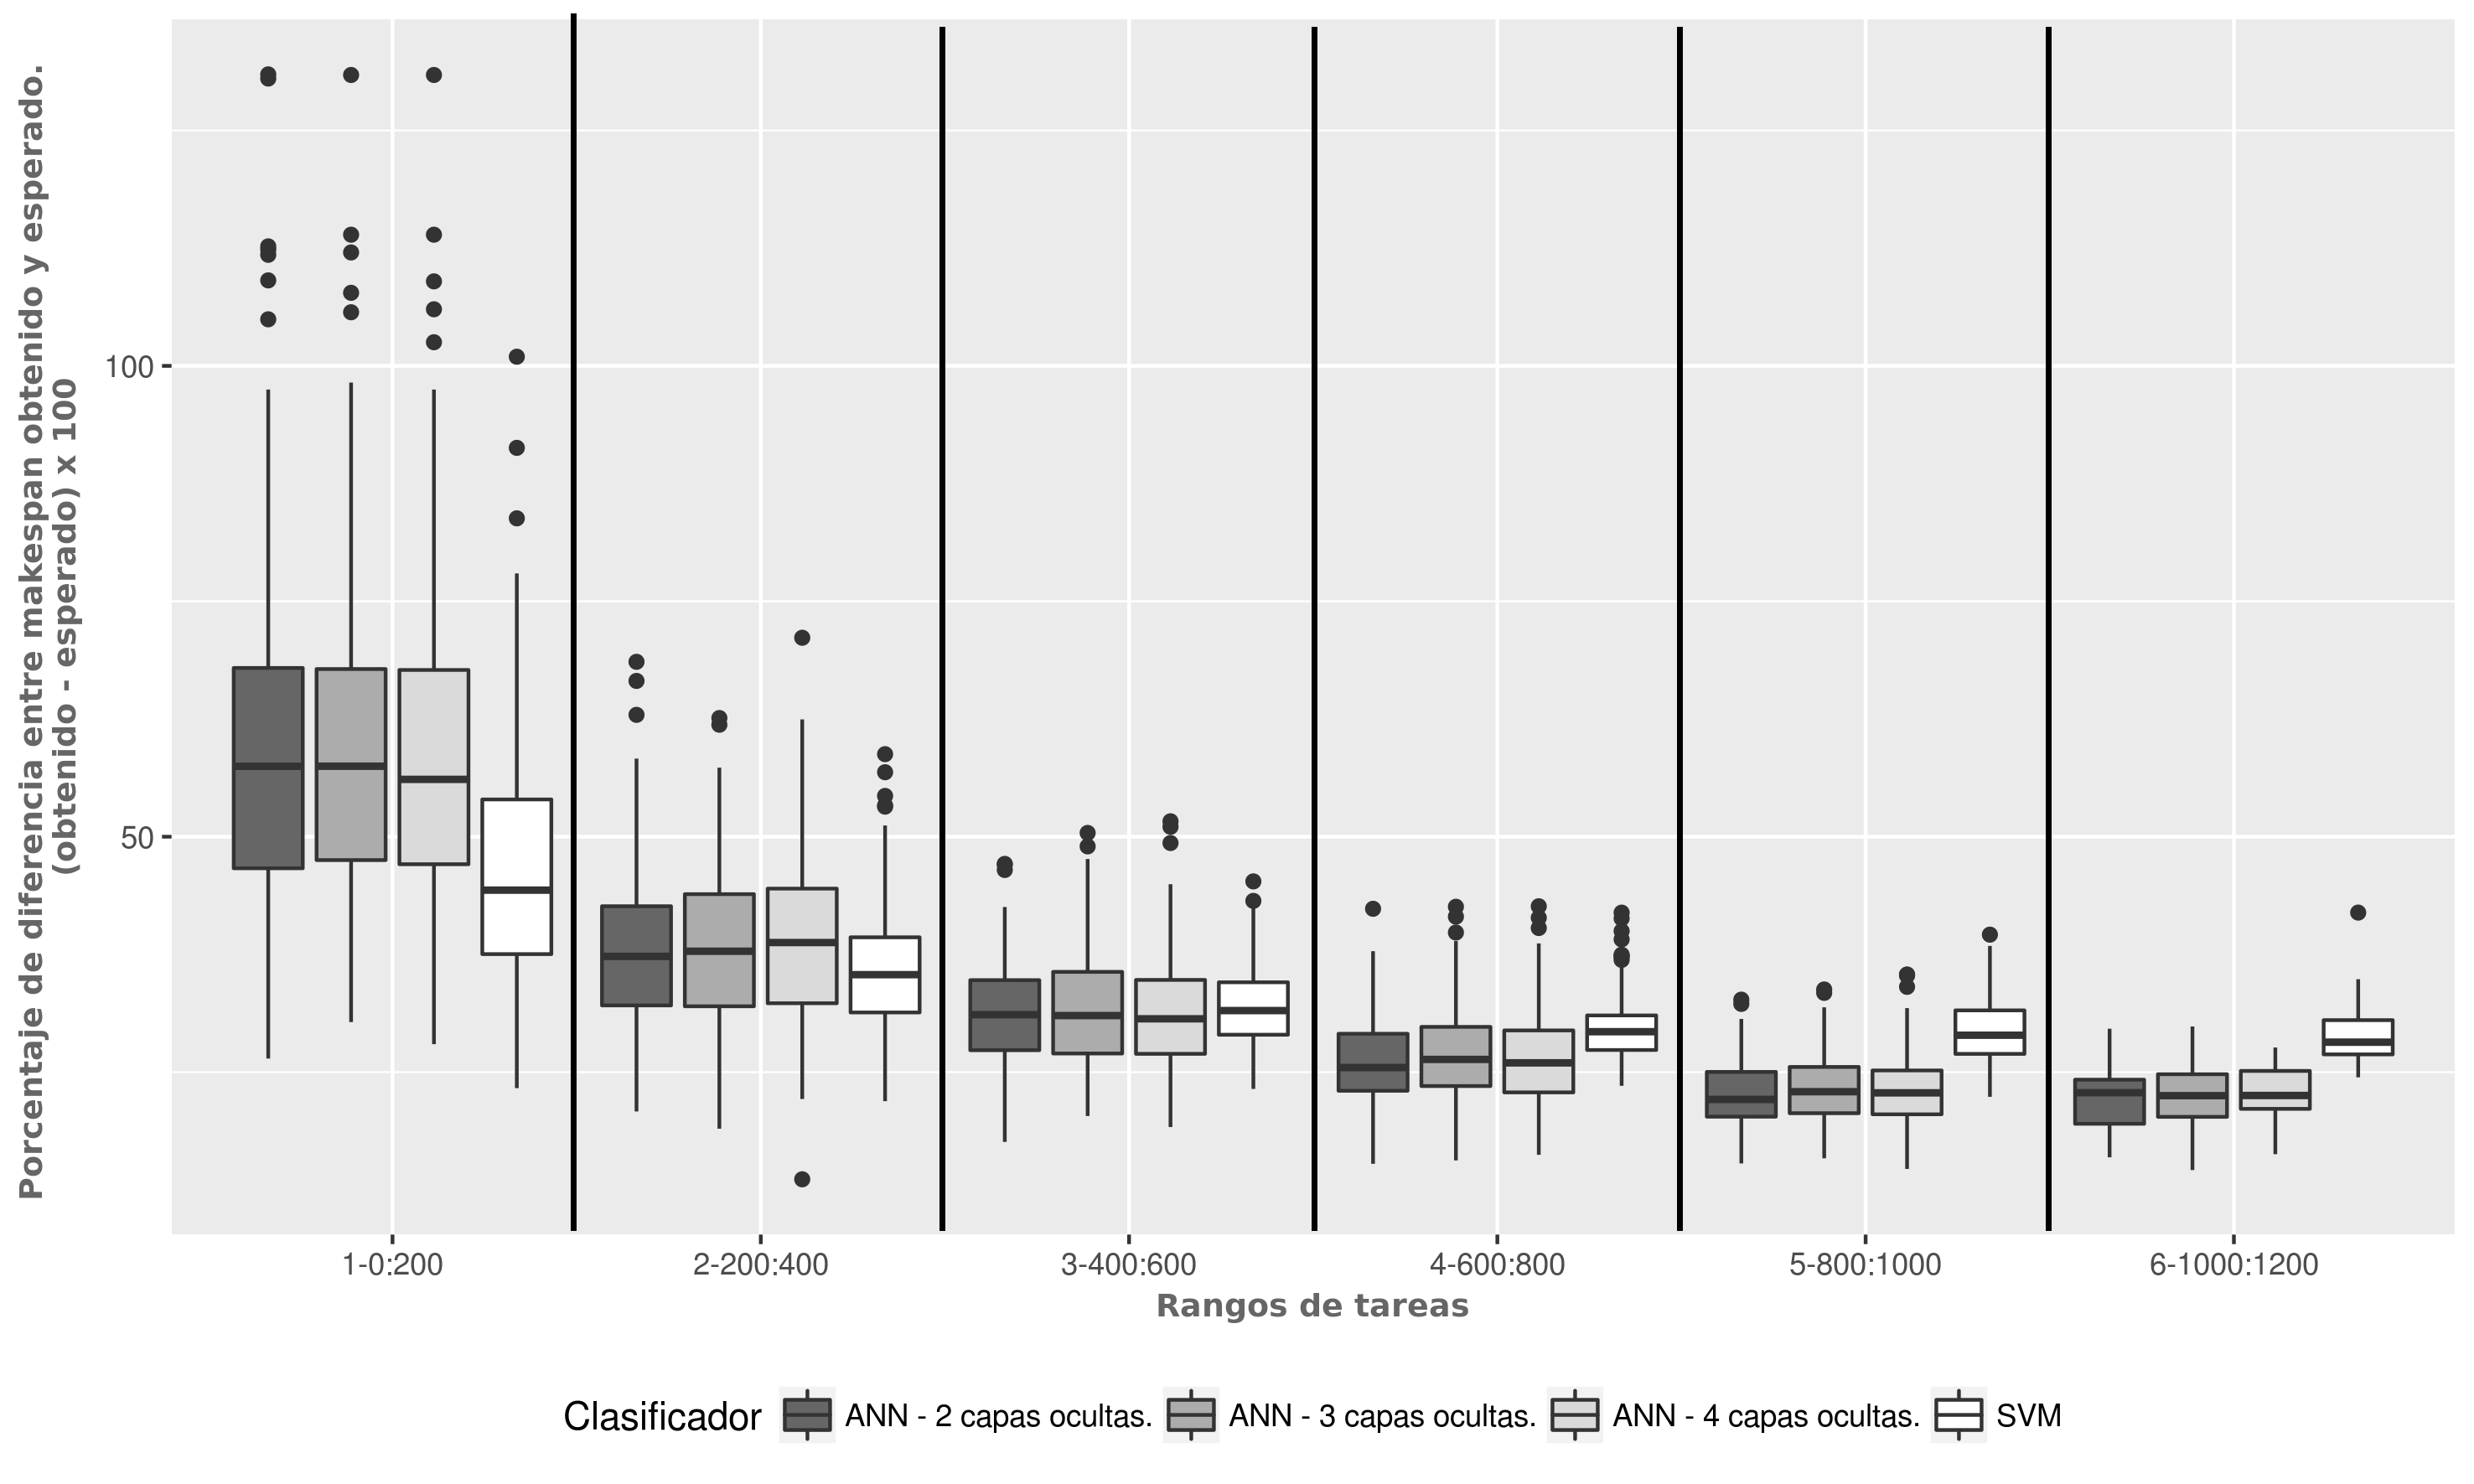
\includegraphics[width=\columnwidth]{imagenes/comparacion_anns_identity_2.png}
  \caption{Comparación de  la diferencia porcentual  de los resultados de \textit{makespan} para redes neuronales con función de activación \textit{identity} y para SVM, con respecto al \textit{makespan} obtenido por el algoritmo Min-Min. Se comparan redes neuronales de 2, 3 y 4 capas. Así también se muestran los resultados obtenidos con el algoritmo de SVM.}
  \label{fig:identity234}
\end{figure}}

\newpage % orphaned line.

\textsc{\begin{figure}[H]
  \centering
  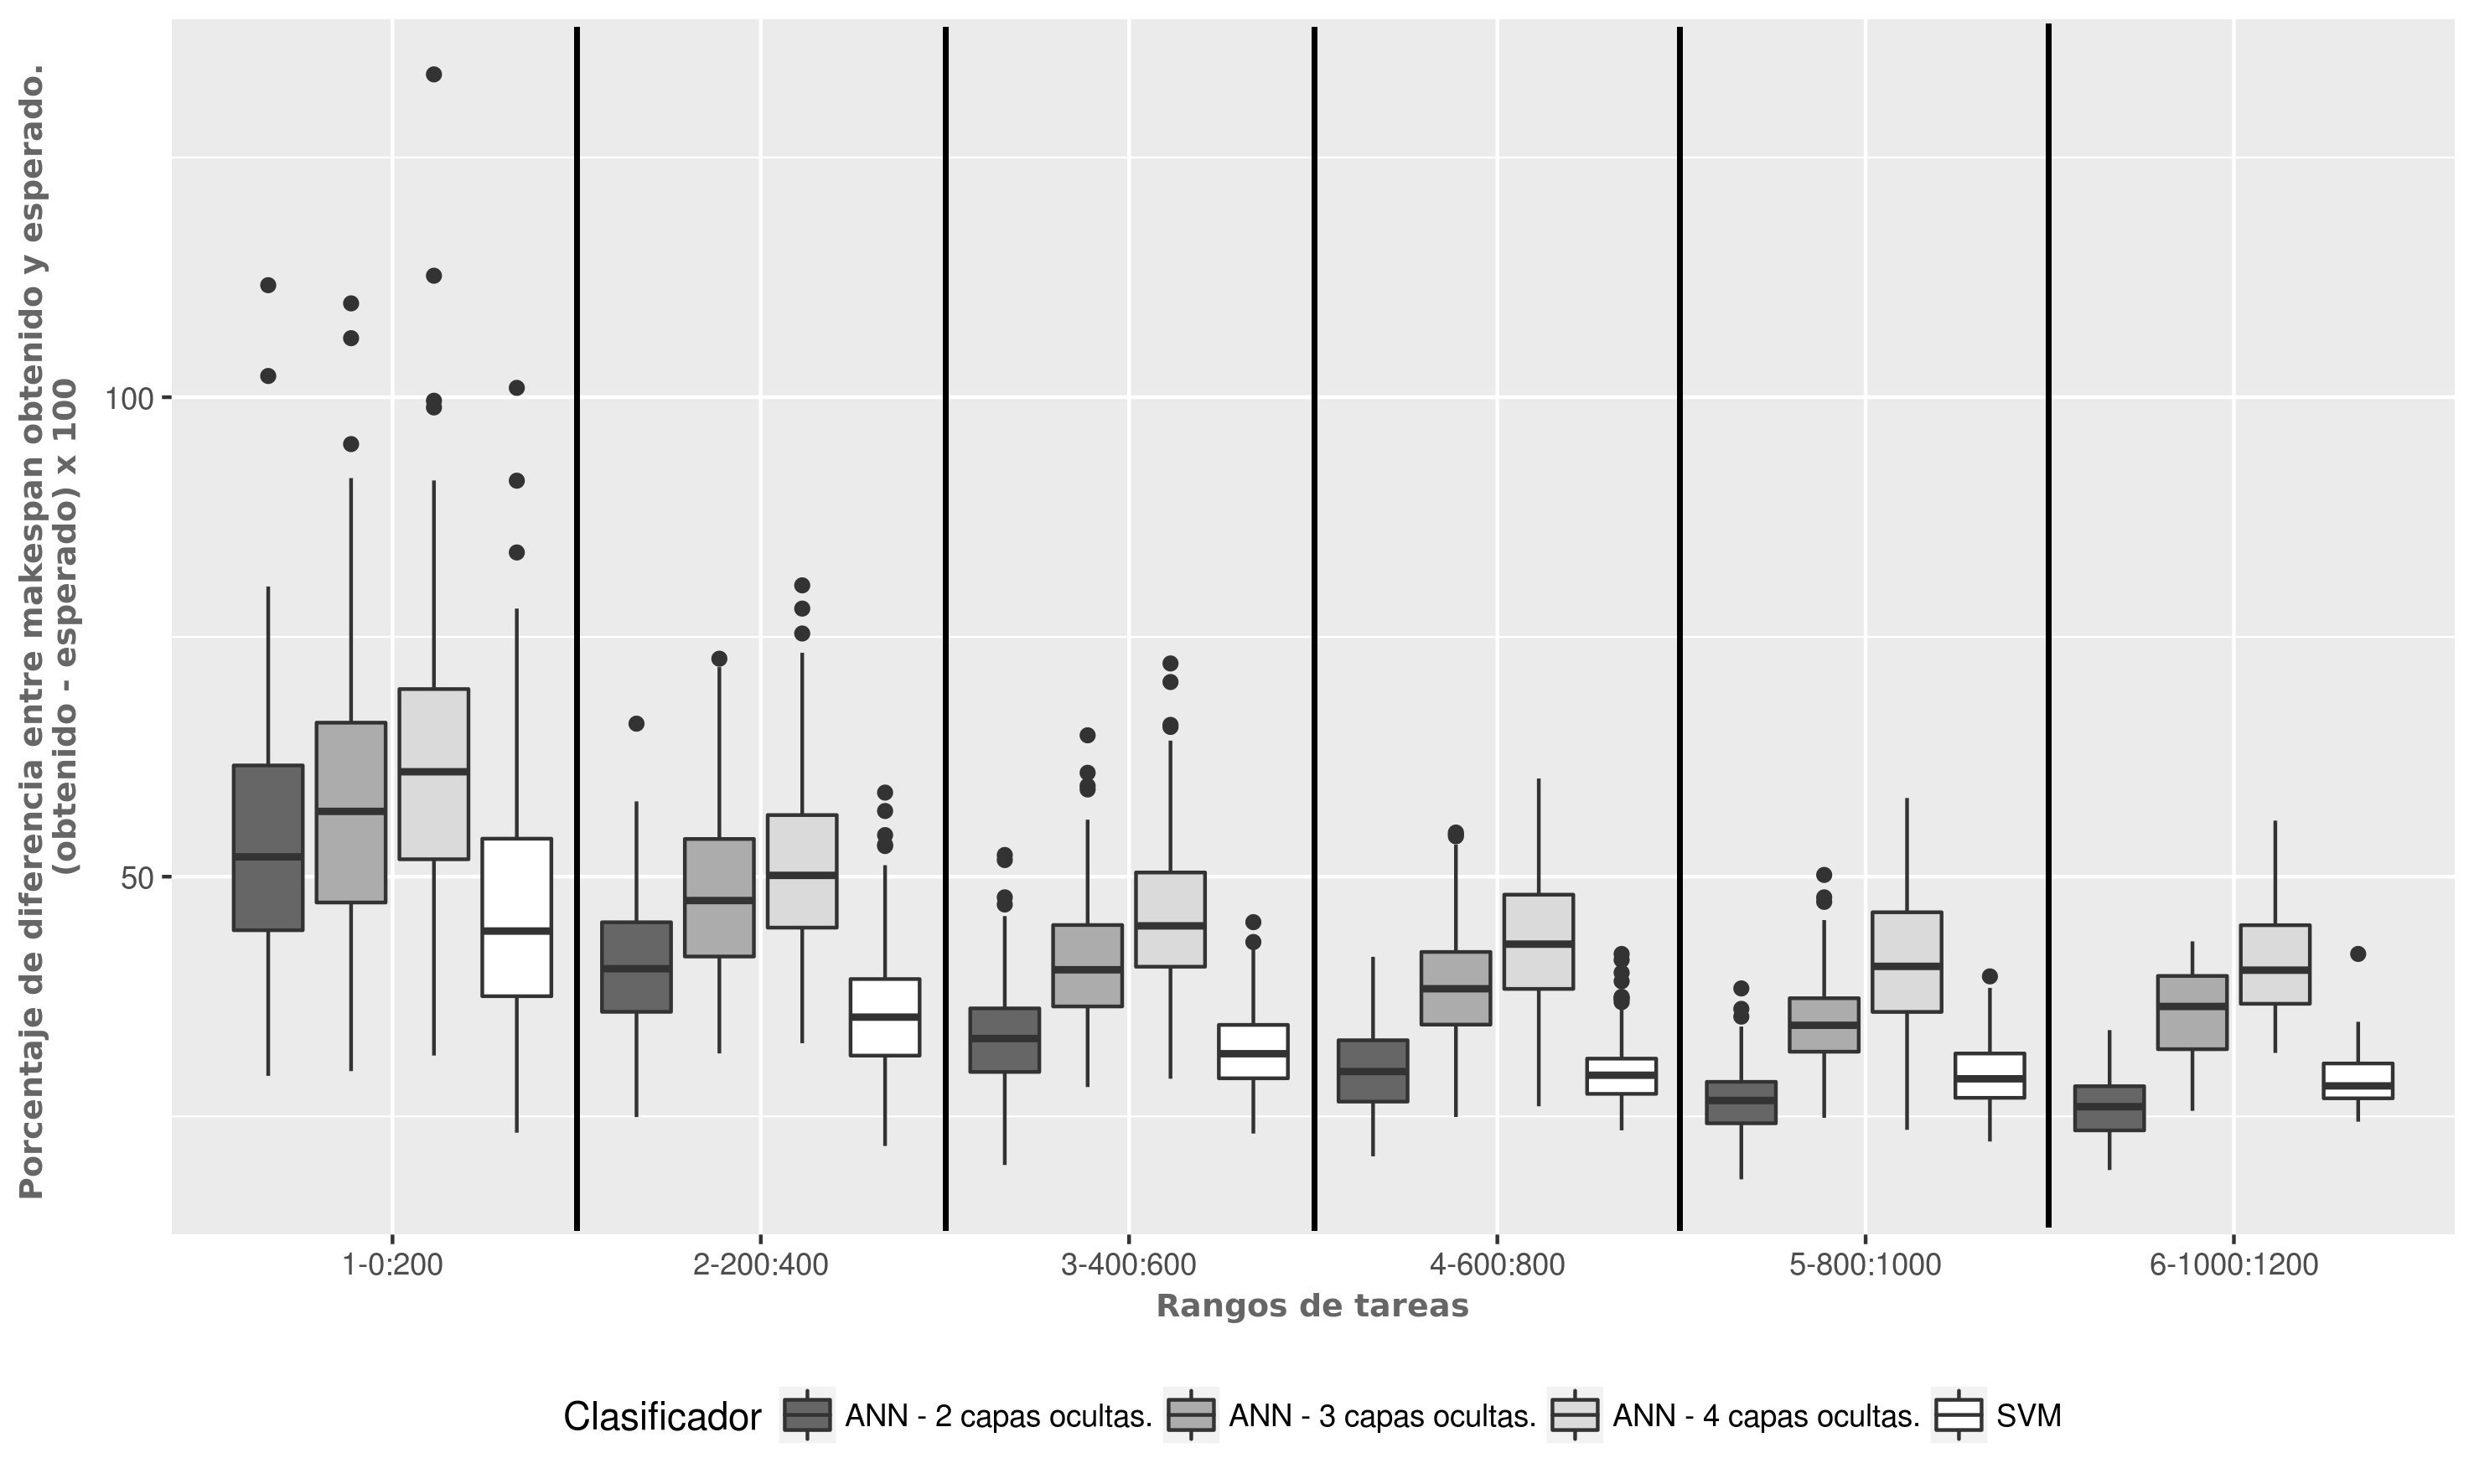
\includegraphics[width=\columnwidth]{imagenes/comparacion_anns_tanh_2.png}
  \caption{Comparación de  la diferencia porcentual  de los resultados de \textit{makespan} para redes neuronales con función de activación \textit{tanh} y para SVM, con respecto al \textit{makespan} obtenido por el algoritmo Min-Min.
Se comparan redes neuronales de 2, 3 y 4 capas.
Así también se muestran los resultados obtenidos con el algoritmo de SVM.}
  \label{fig:tanh234}
\end{figure}}

\newpage % orphaned line.

\section{Red neuronal con activación \textit{relu} de dos capas ocultas}

La Figura \ref{fig:relu_makespan} muestra la diferencia porcentual de \textit{makespan} entre la red neuronal de dos capas ocultas con función de activación \textit{relu} y la SVM con respecto al \textit{makespan} esperado.
Como ya se observó, la SVM muestra valores más próximos a los valores esperados que la red neuronal. 

\paragraph{} Por otro lado, la Figura \ref{fig:relu_accuracy} muestra la precisión de la clasificación para ambos clasificadores.
Se observa que la precisión en la clasificación aumenta a medida que la dimensión de las instancias de prueba aumenta, tanto para la red neuronal como para la SVM. 

\begin{figure}[H]
  \centering
  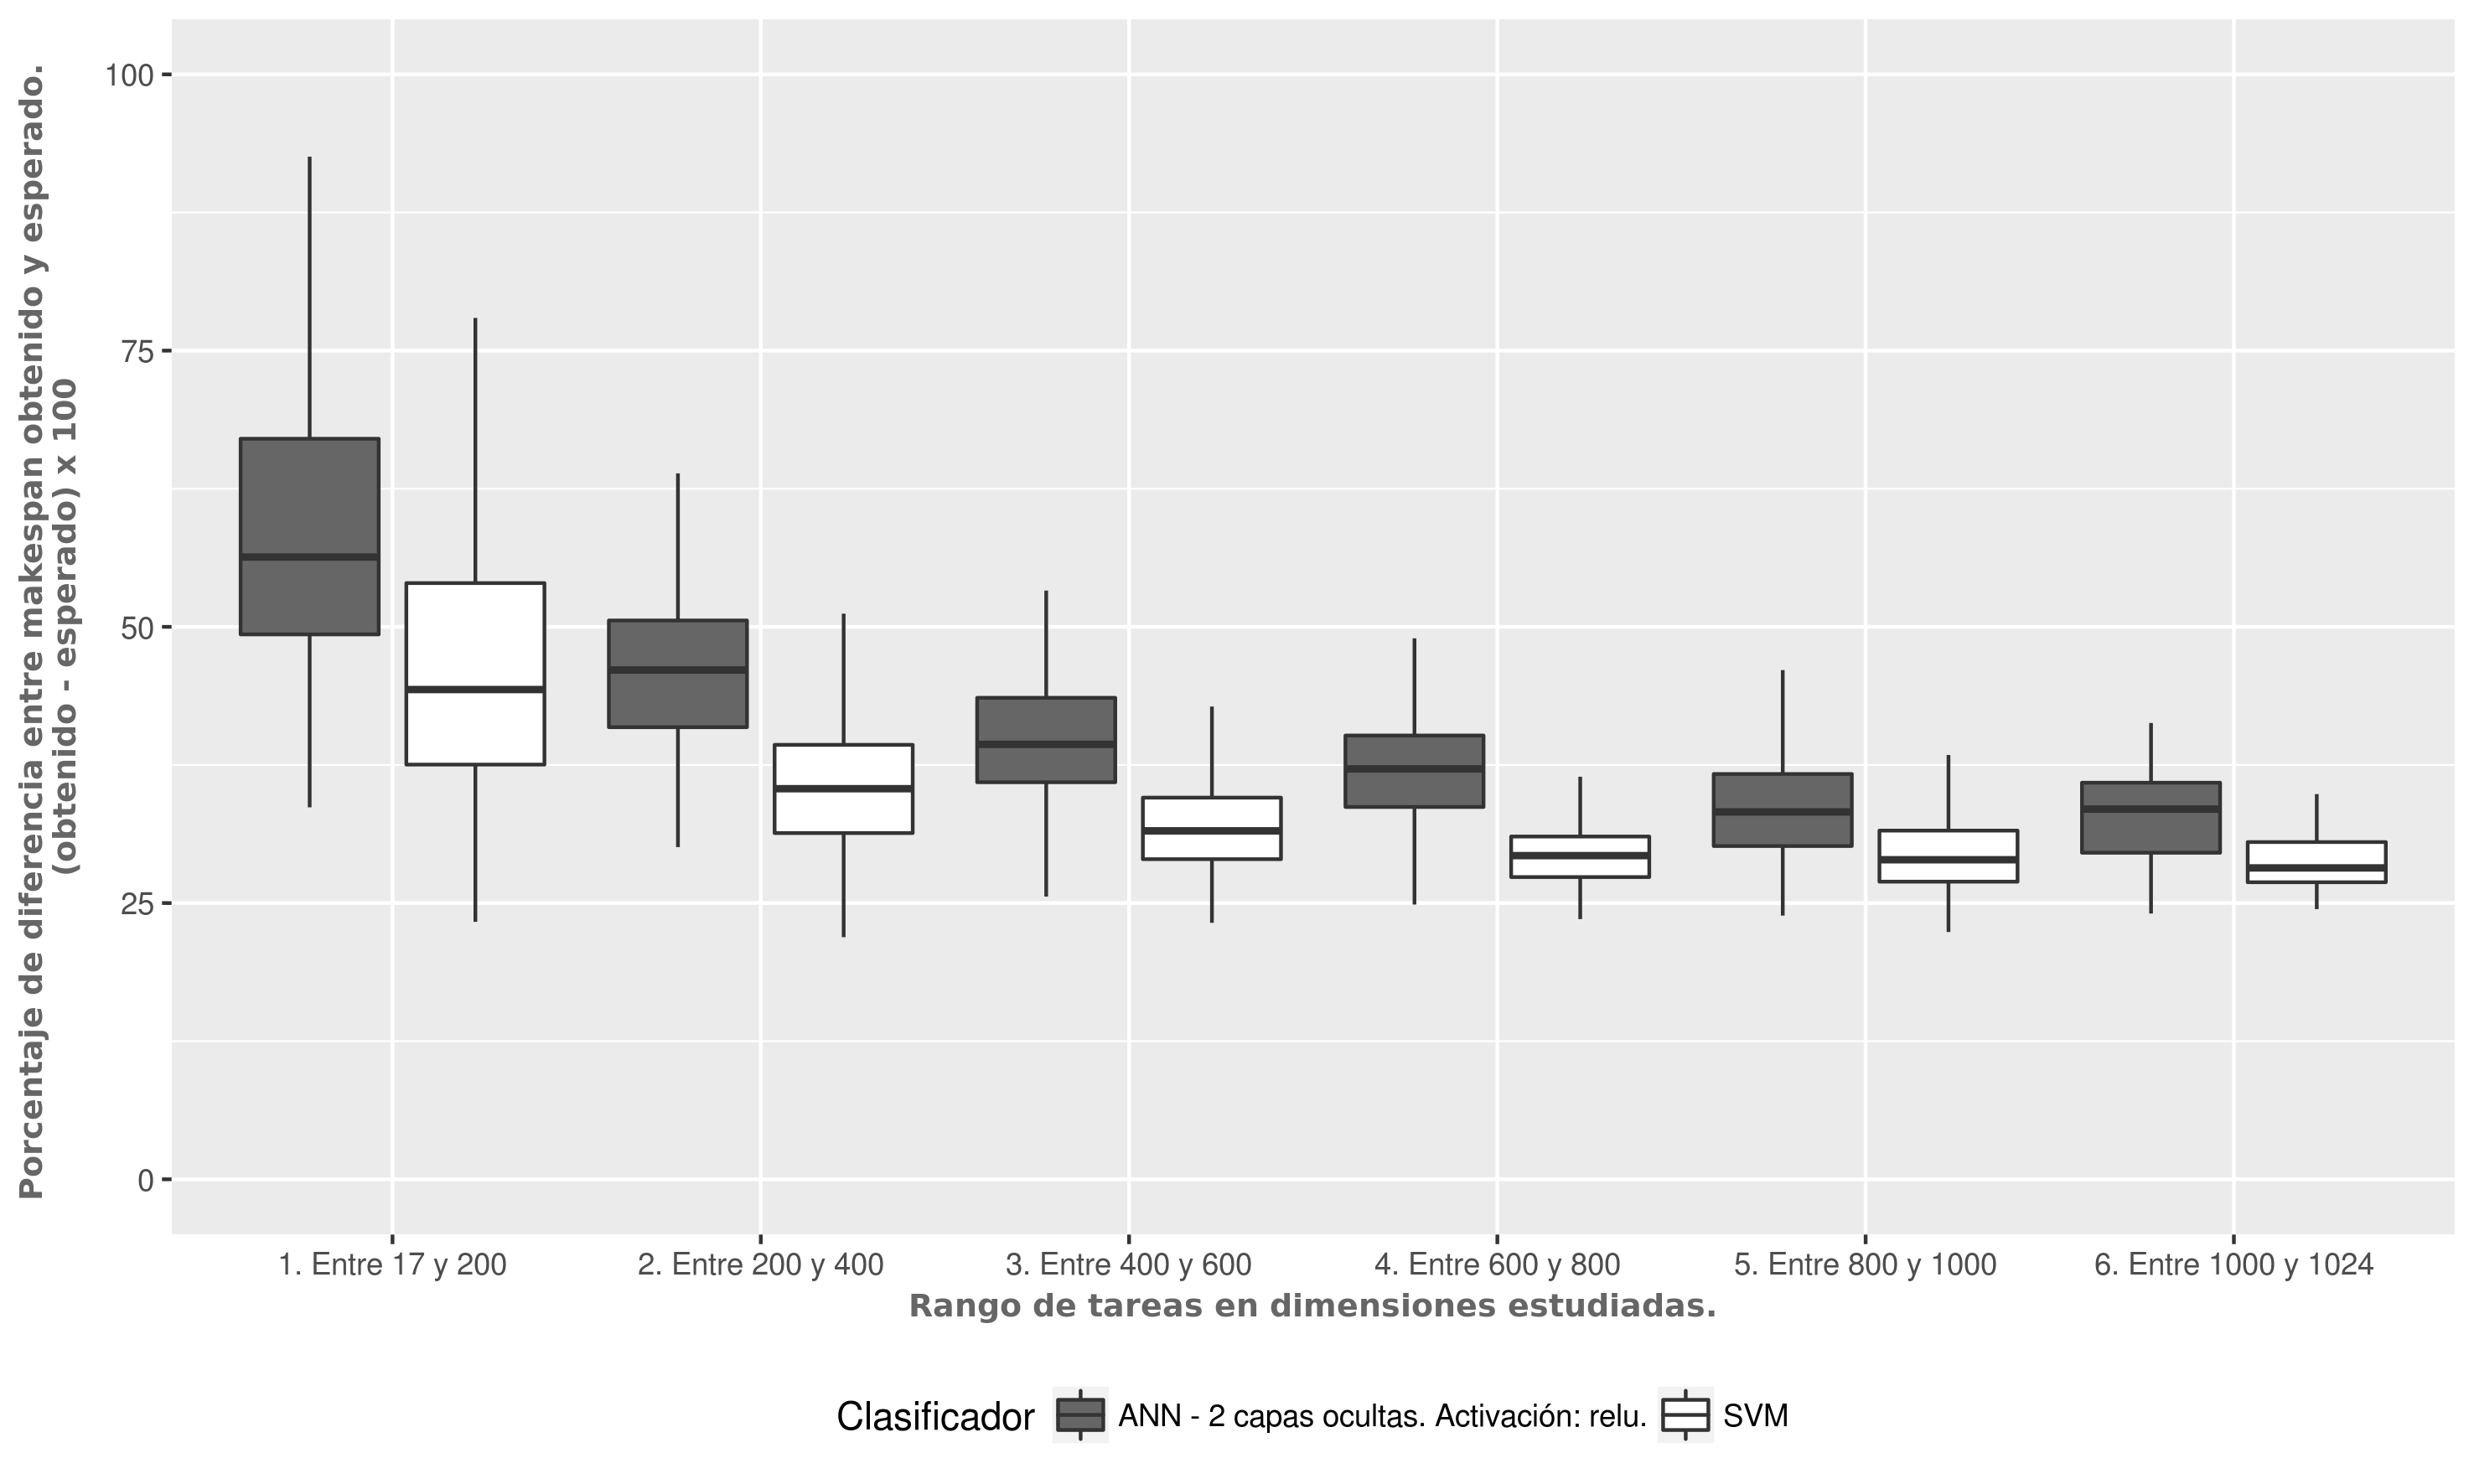
\includegraphics[width=\columnwidth]{imagenes/relu/2_medianas_diferenciasann_2_capas_ocultas_relu.png}
  \caption{Comparación de la diferencia porcentual de \textit{makespan} para la red neuronal con activación \textit{relu}, de dos capas ocultas con respecto a los valores esperados obtenidos con el algoritmo Min-Min.
Así también se muestran los resultados obtenidos para la SVM.
Los resultados se muestran divididos en rangos de dimensión desde $ 17 \times 16$ a $ 1024 \times 16$.}
  \label{fig:relu_makespan}
\end{figure}

\newpage % orphaned line.

\paragraph{}La precisión de la red neuronal es levemente mayor que la precisión de la SVM.
Esto, en comparación con la diferencia de \textit{makespan} de la Figura \ref{fig:relu_makespan}, es de interés dado que, si bien la precisión de la red neuronal es levemente mejor, la SVM genera mejores resultados en términos de \textit{makespan}.
Este escenario también fue identificado para las demás redes neuronales en las cuales se profundizaron los estudios. 

\paragraph{} Para poder explicar lo antedicho, se calculó el porcentaje de selección de mejores máquinas para ambos clasificadores, como se menciona en la Sección \ref{chapter-implementacion:clasificacion}.
La Figura \ref{fig:relu_maquinas_mejores} muestra dicha métrica para ambos clasificadores.
Se puede observar que SVM elige más máquinas con menor tiempo de ejecución que la red neuronal, cuando  se seleccionan máquinas diferentes a las esperadas. 

\begin{figure}[H]
  \centering
  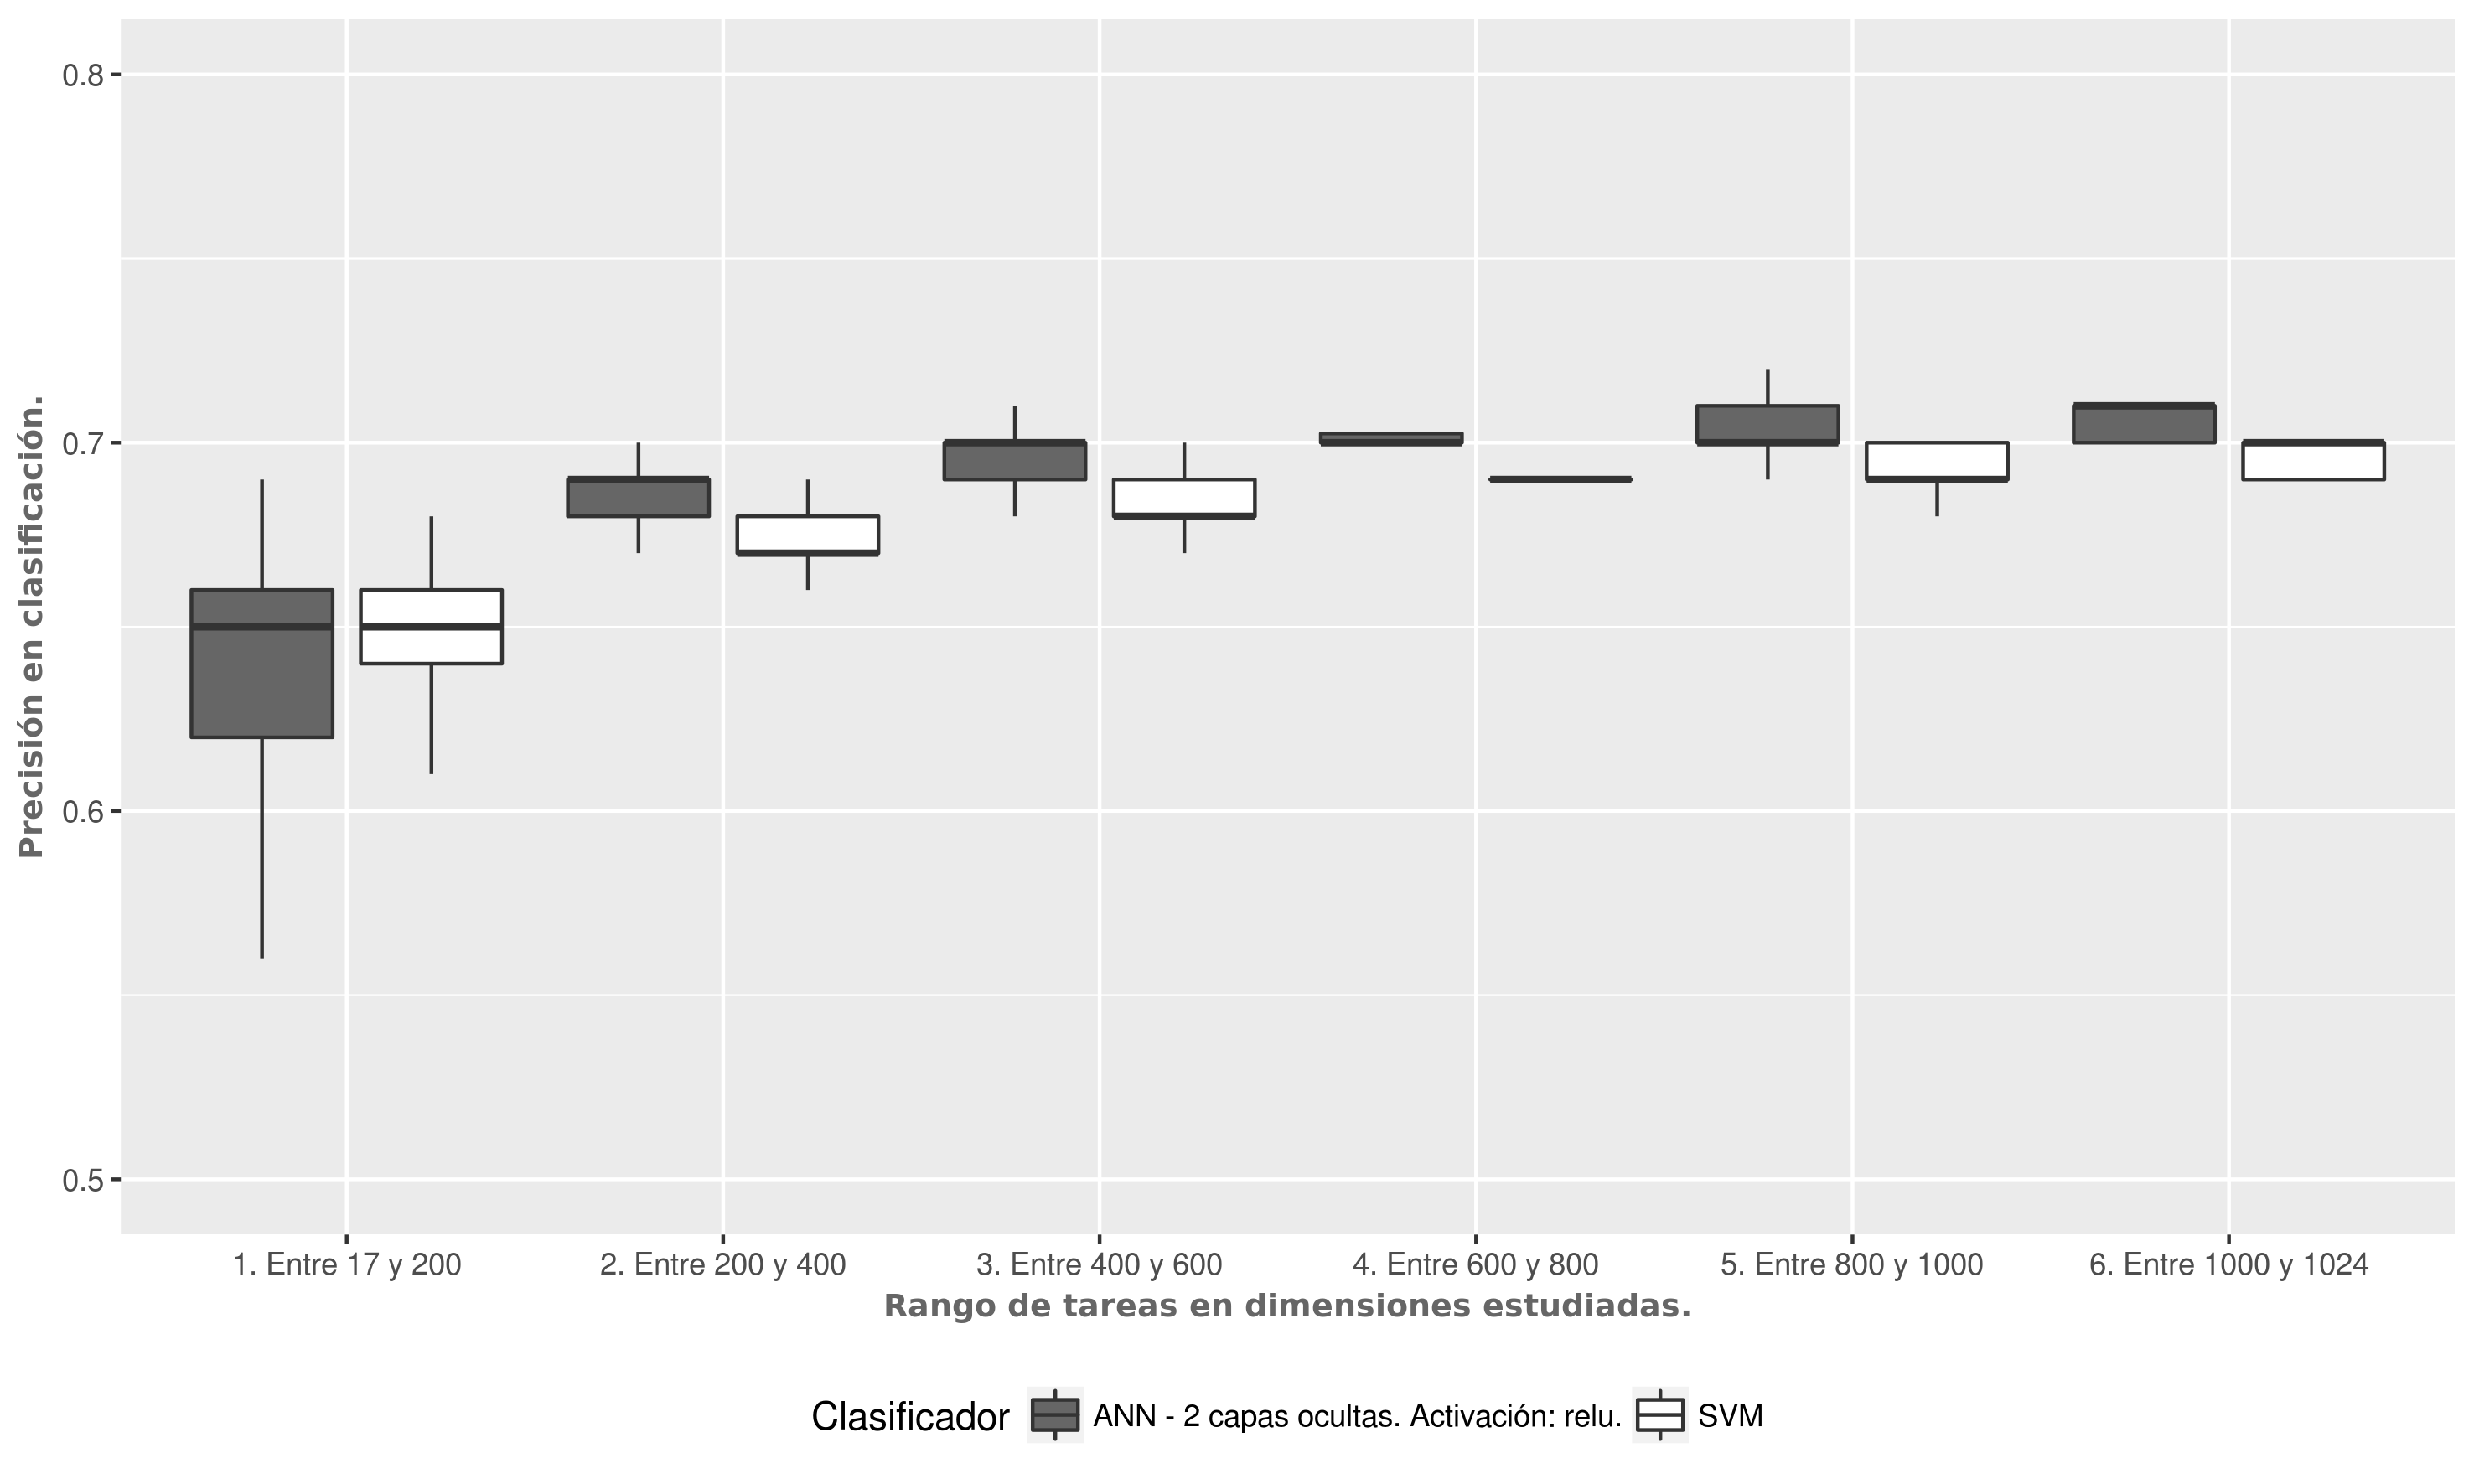
\includegraphics[width=\columnwidth]{imagenes/relu/3_accuracy_ann_2_capas_ocultas_relu.png}
  \caption{Precisión en clasificación para la red neuronal con función de activación \textit{relu} de dos capas ocultas y para la SVM.
Los resultados se muestran divididos en rangos de dimensión desde $ 17 \times 16$ a $ 1024 \times 16$.}
  \label{fig:relu_accuracy}
\end{figure}

\newpage % orphaned line.

\begin{figure}[H]
  \centering
  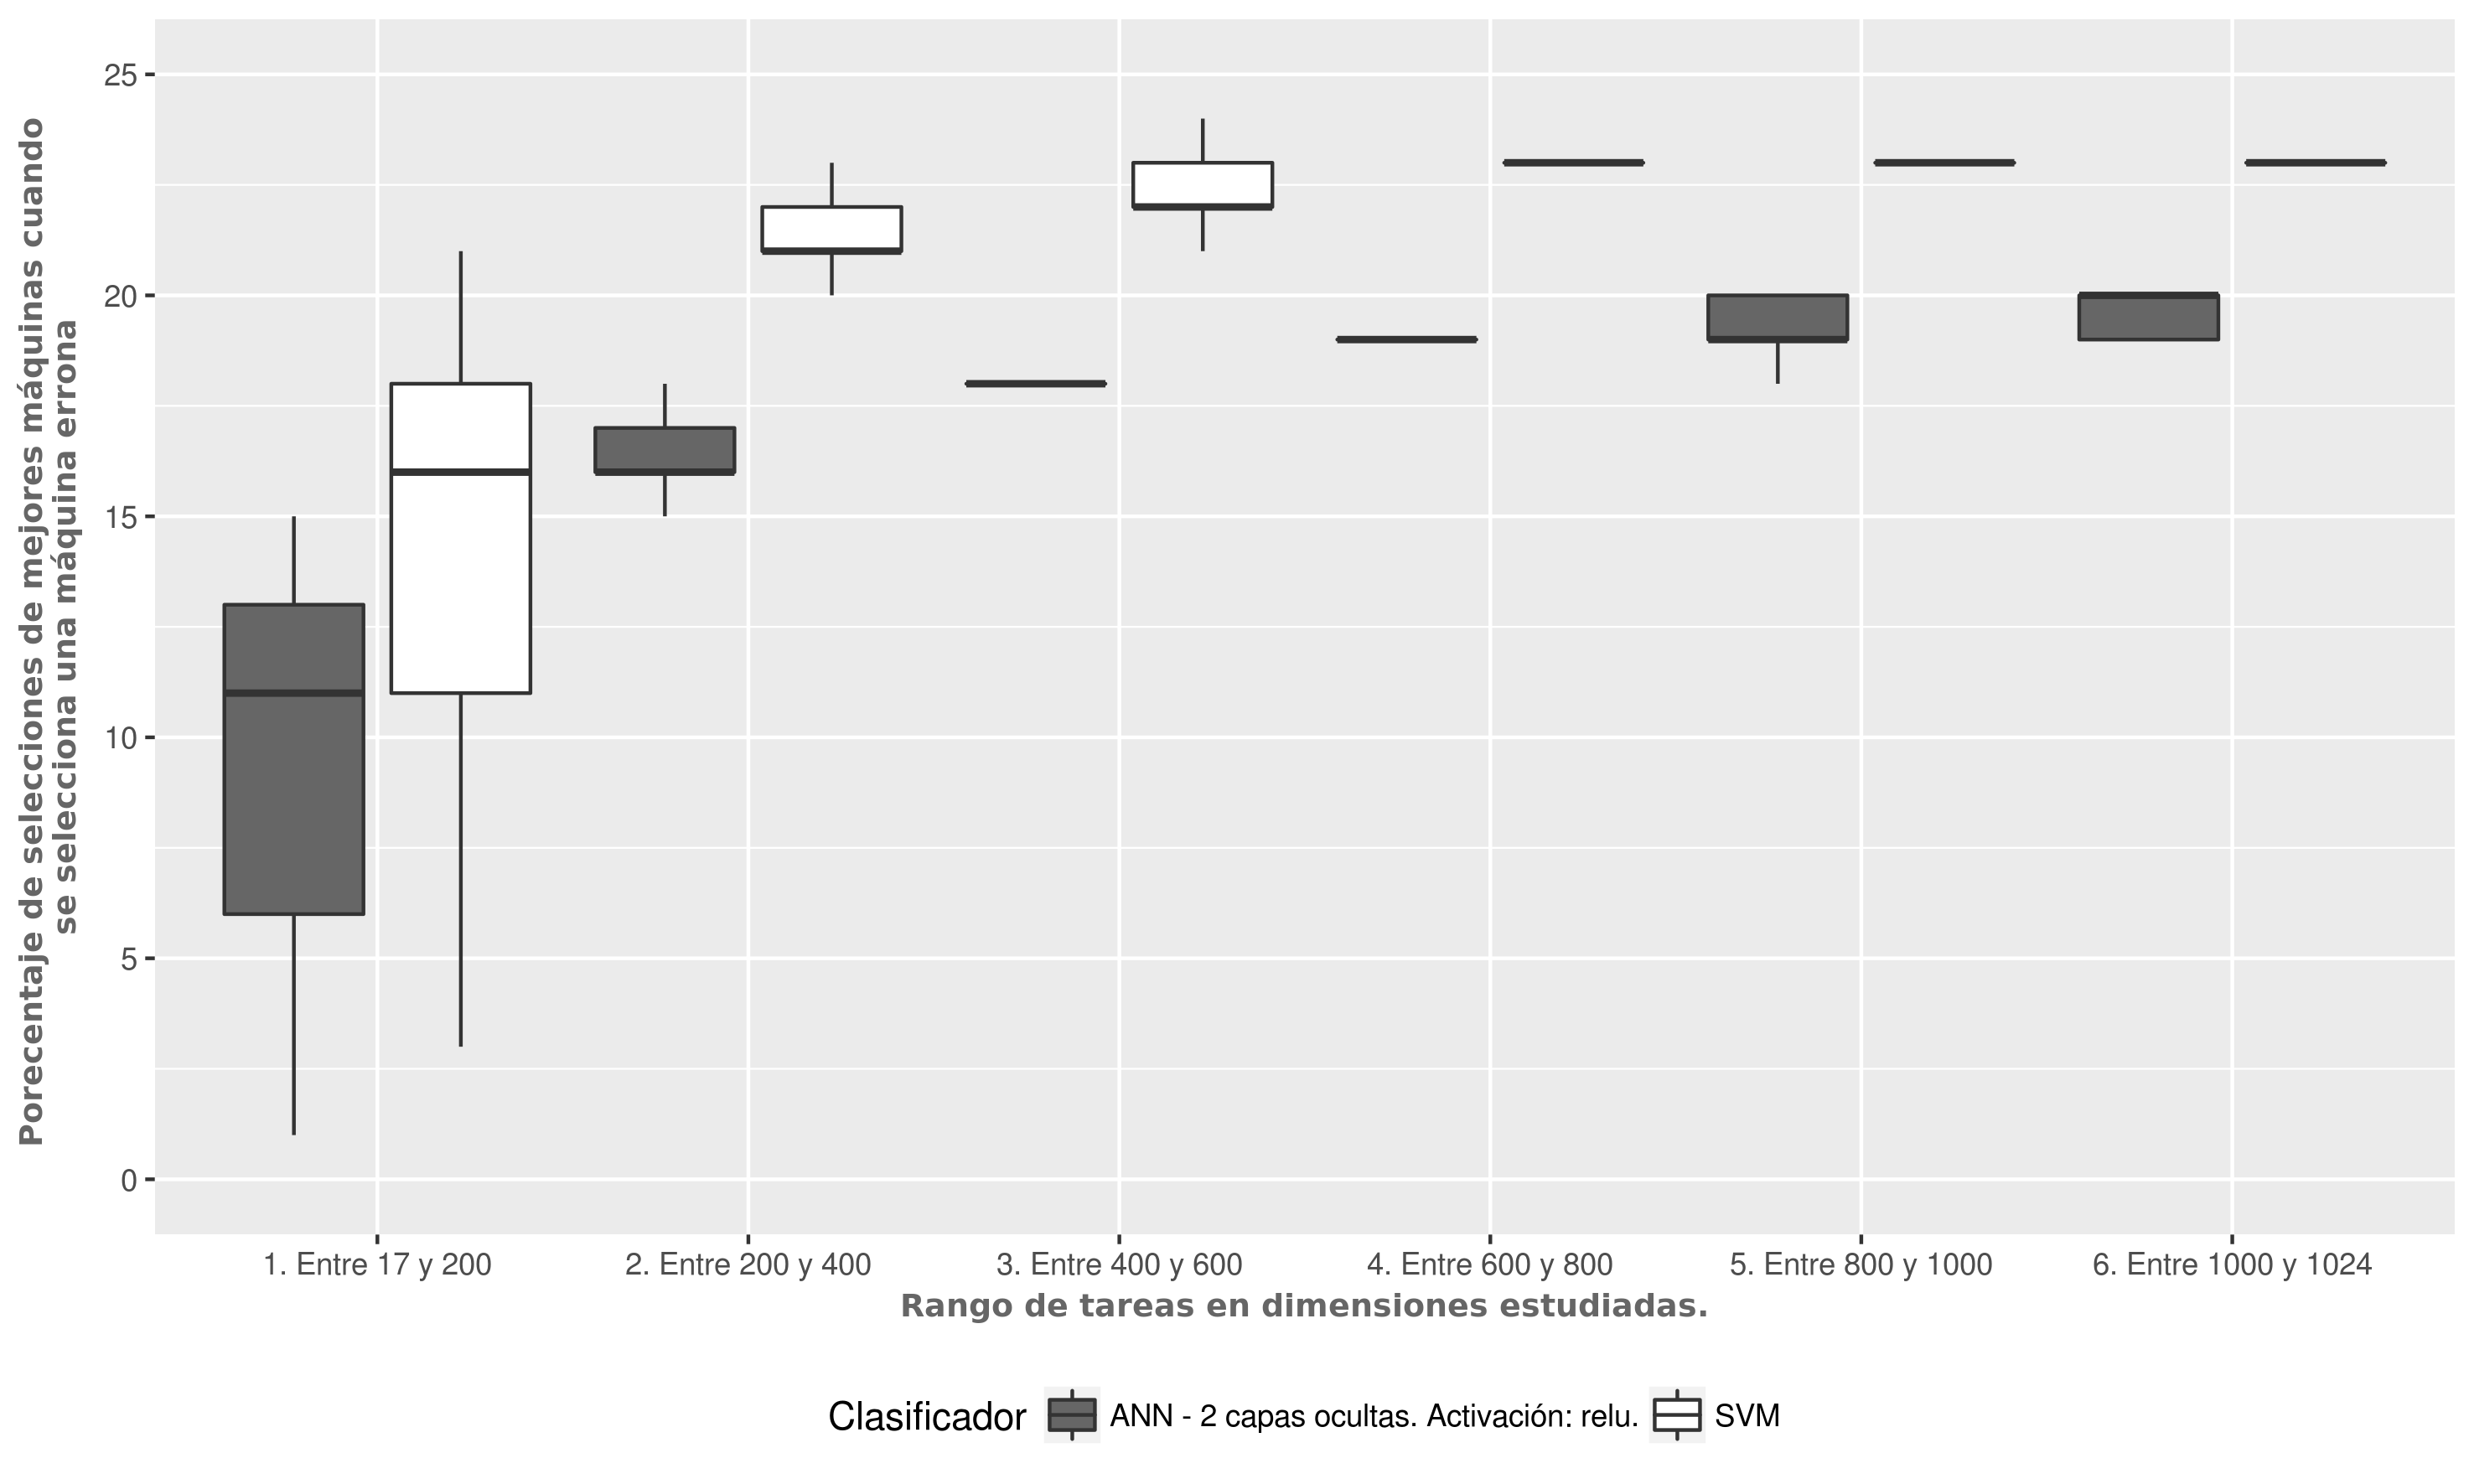
\includegraphics[width=\columnwidth]{imagenes/relu/4_porcentaje_maquinas_mejores_ann_2_capas_ocultas_relu.png}
  \caption{Porcentaje de selección de máquinas mejores frente a una selección diferente a la esperada para la red neuronal con activación \textit{relu} de dos capas ocultas y para la SVM.}
  \label{fig:relu_maquinas_mejores}
\end{figure}

\newpage % orphaned line.
 
\section{Red neuronal con activación \textit{identity} de dos capas ocultas}

\paragraph{} La Figura \ref{fig:identity_makespan} muestra la diferencia porcentual de \textit{makespan} para la red neuronal con función de activación \textit{identity} y la SVM, con respecto a los resultados esperados obtenidos con el algoritmo Min-Min.
Se observa que para dimensiones mayores a $ 400 \times 16$, la red neuronal conduce a levemente mejores valores de \textit{makespan} que la SVM.
En este caso, la precisión en la clasificación, que se observa en la Figura \ref{fig:identity_accuracy}, no tiene diferencias sustanciales. 

\begin{figure}[H]
  \centering
  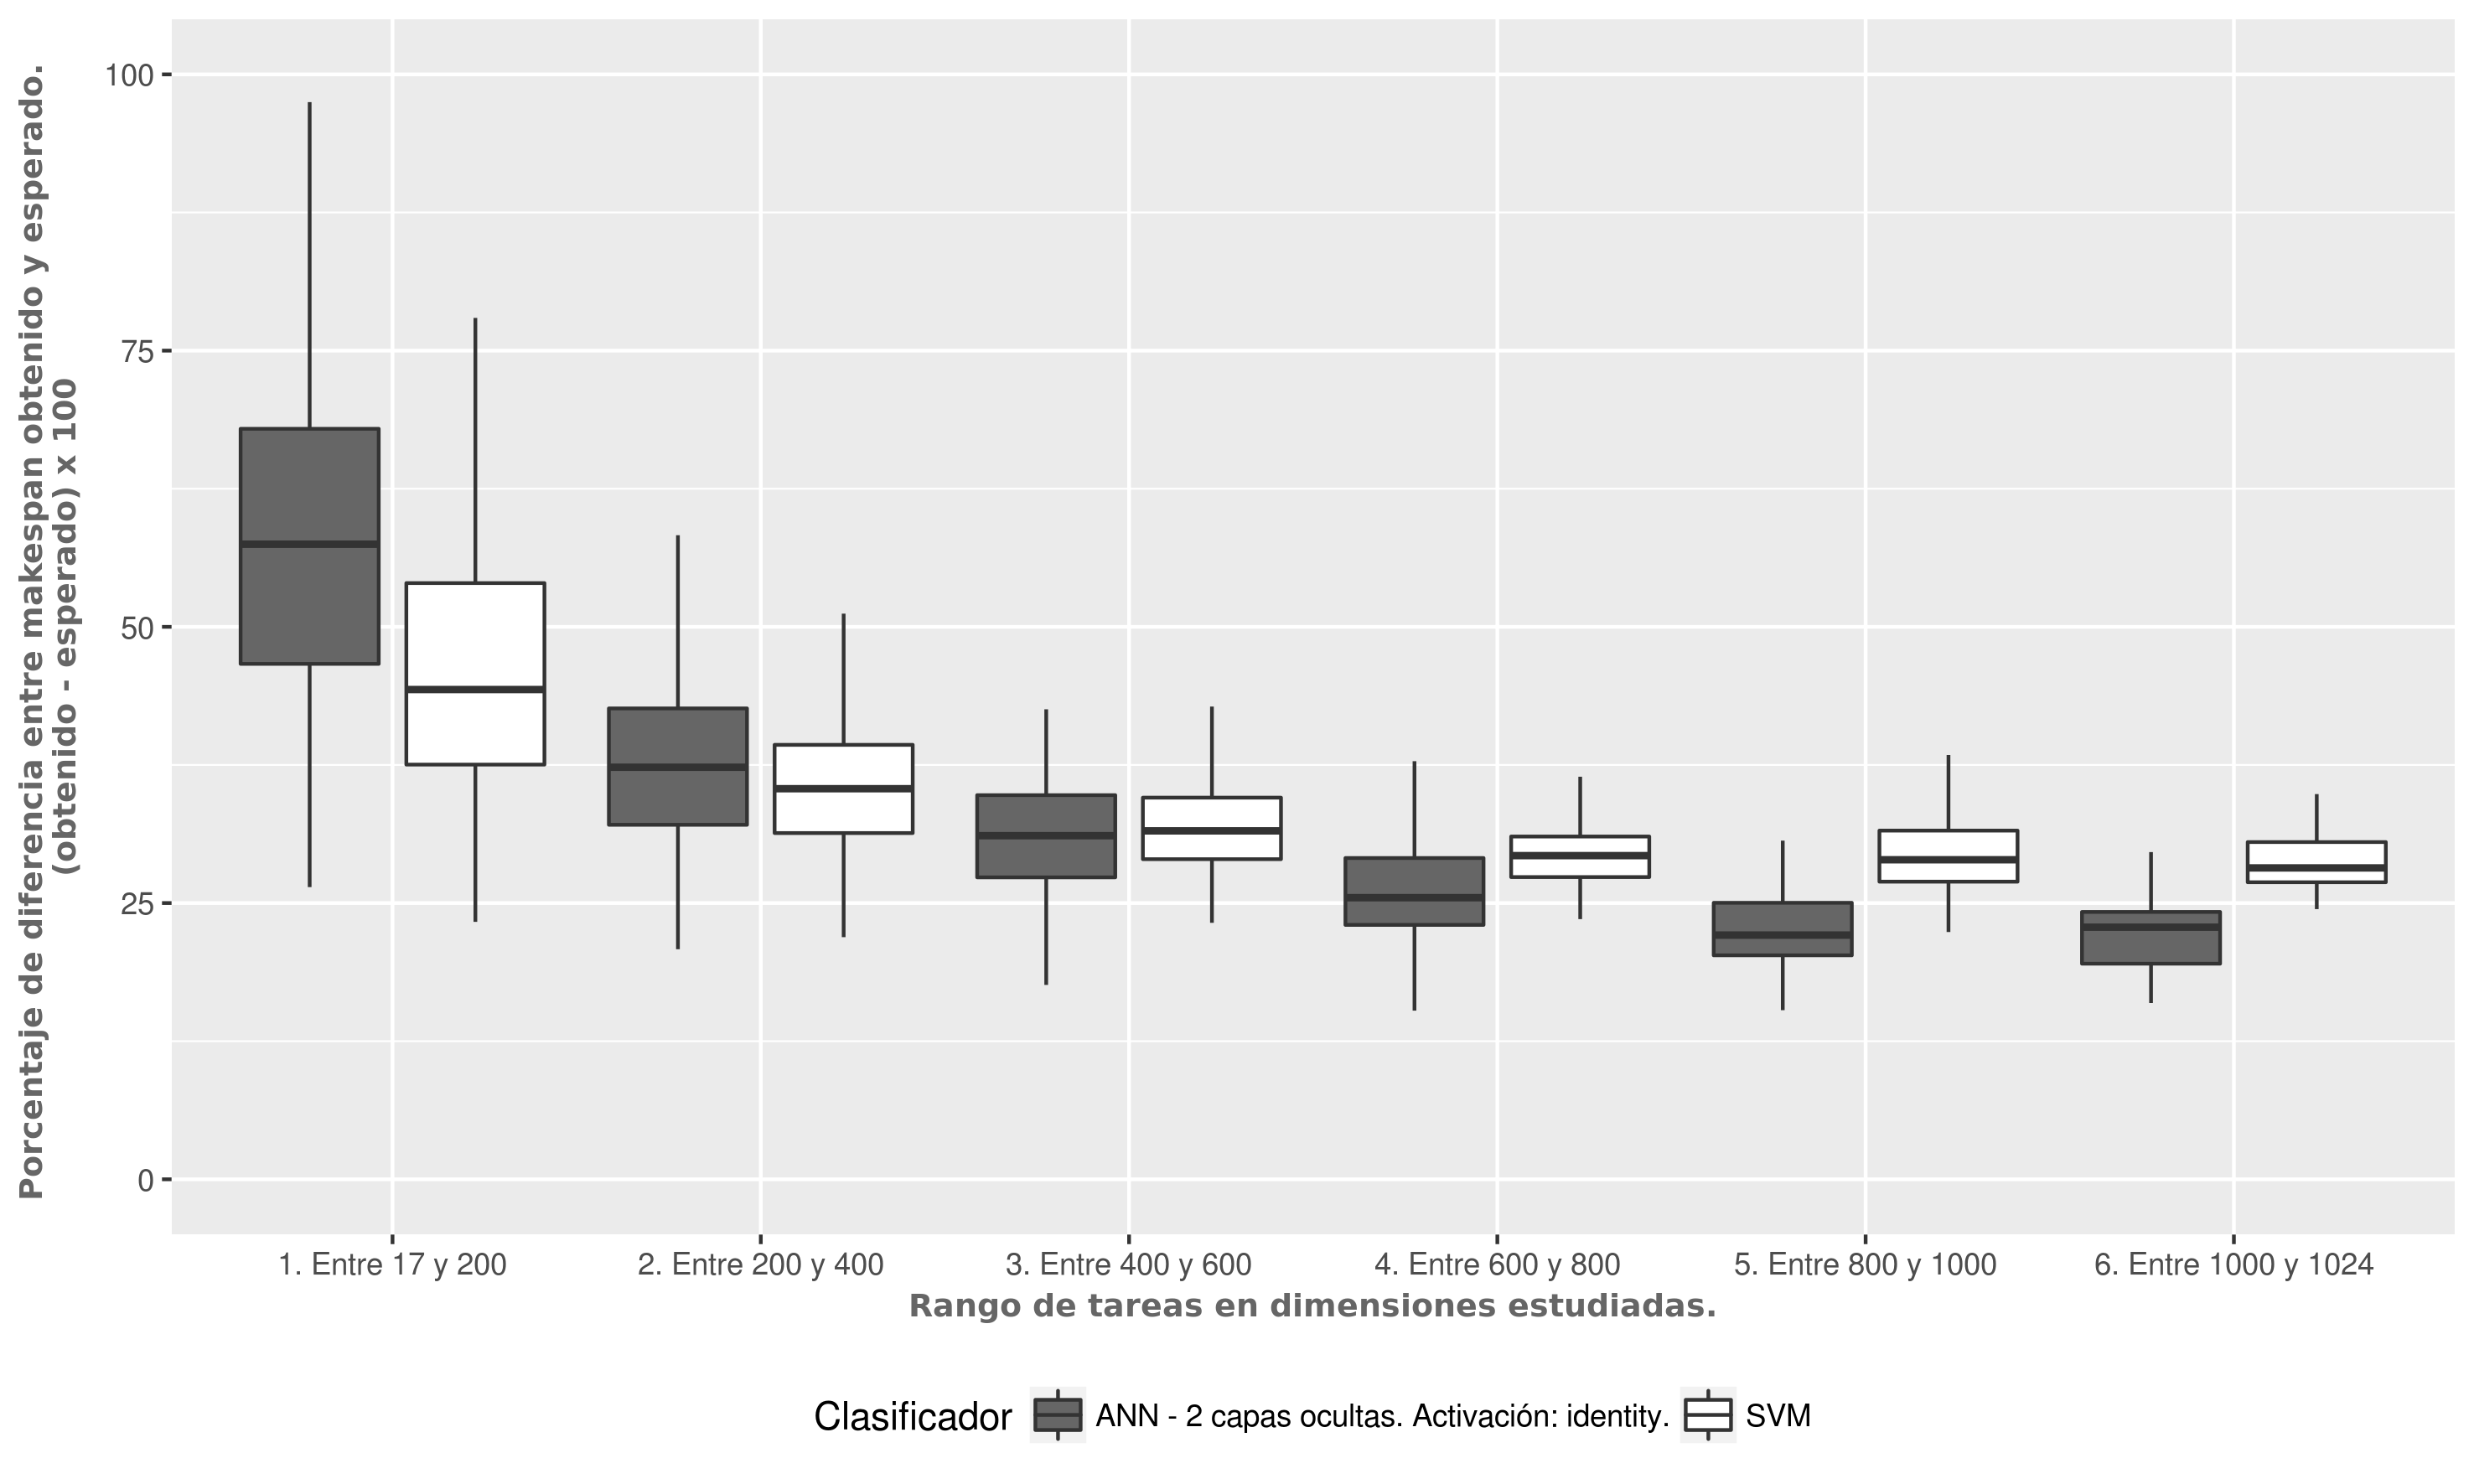
\includegraphics[width=\columnwidth]{imagenes/identity/2_medianas_diferenciasann_2_capas_ocultas_identity.png}
  \caption{Comparación de la diferencia porcentual de \textit{makespan} para la red neuronal con activación \textit{identity}, de dos capas ocultas con respecto a los valores esperados obtenidos con el algoritmo Min-Min.
Así también se muestran los resultados obtenidos para la SVM.
Los resultados se muestran divididos en rangos de dimensión desde $ 17 \times 16$ a $ 1024 \times 16$}
  \label{fig:identity_makespan}
\end{figure}

\newpage % orphaned line.

\begin{figure}[H]
  \centering
  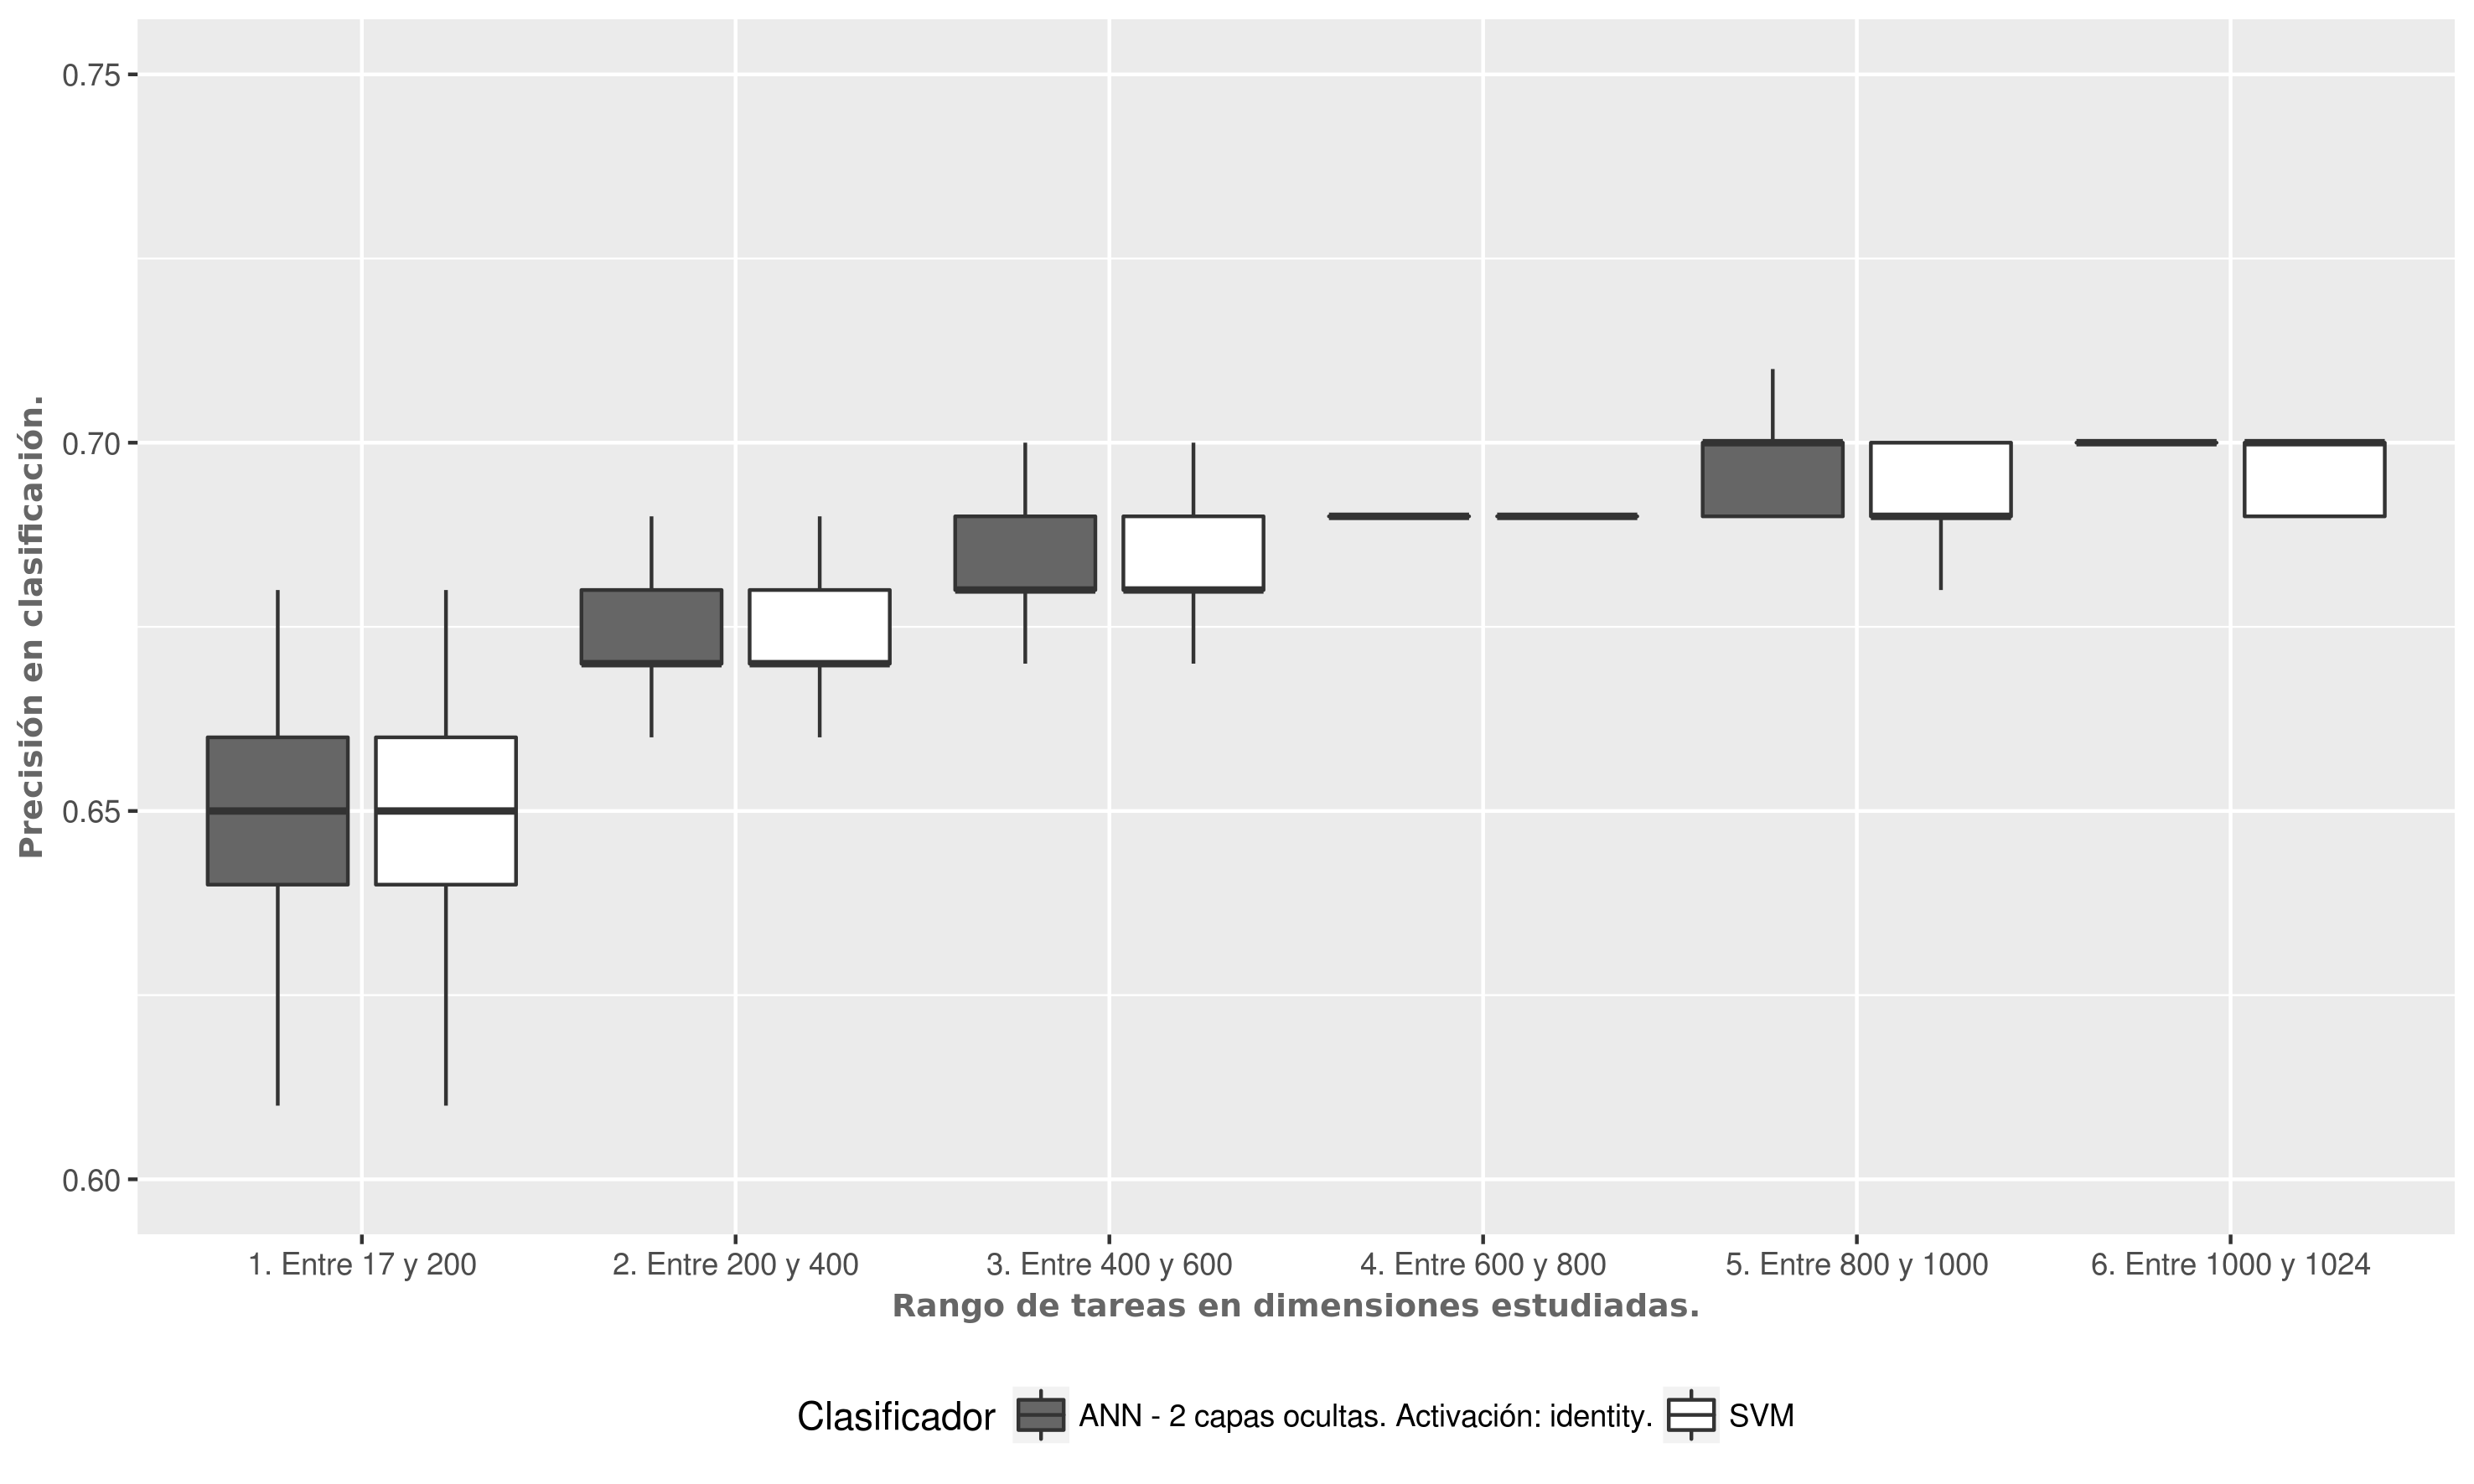
\includegraphics[width=\columnwidth]{imagenes/identity/3_accuracy_ann_2_capas_ocultas_identity.png}
  \caption{Precisión en clasificación para la red neuronal con función de activación \textit{identity} y para la SVM.
Los resultados se muestran divididos en rangos de dimensión desde $ 17 \times 16$ a $ 1024 \times 16$.}
  \label{fig:identity_accuracy}
\end{figure}

\paragraph{}Al observar el porcentaje de mejores máquinas seleccionadas frente a un error en la Figura \ref{fig:identity_mejores}, se observa que la red neuronal con función de activación \textit{identity} selecciona máquinas más rápidas en proporciones similares a la SVM, a diferencia de los resultados presentados para la red neuronal con función de activación \textit{relu}, que tiende a elegir máquinas más lentas que la SVM frente a un error.
Estos resultados llevan a pensar que el hecho de que la proporción de selección de mejores máquinas por parte de la red neuronal con función de activación \textit{identity} sea mayor que para el caso de \textit{relu}, conduce a una leve disminución del \textit{makespan}. 

\newpage % orphaned line.

\begin{figure}[H]
  \centering
  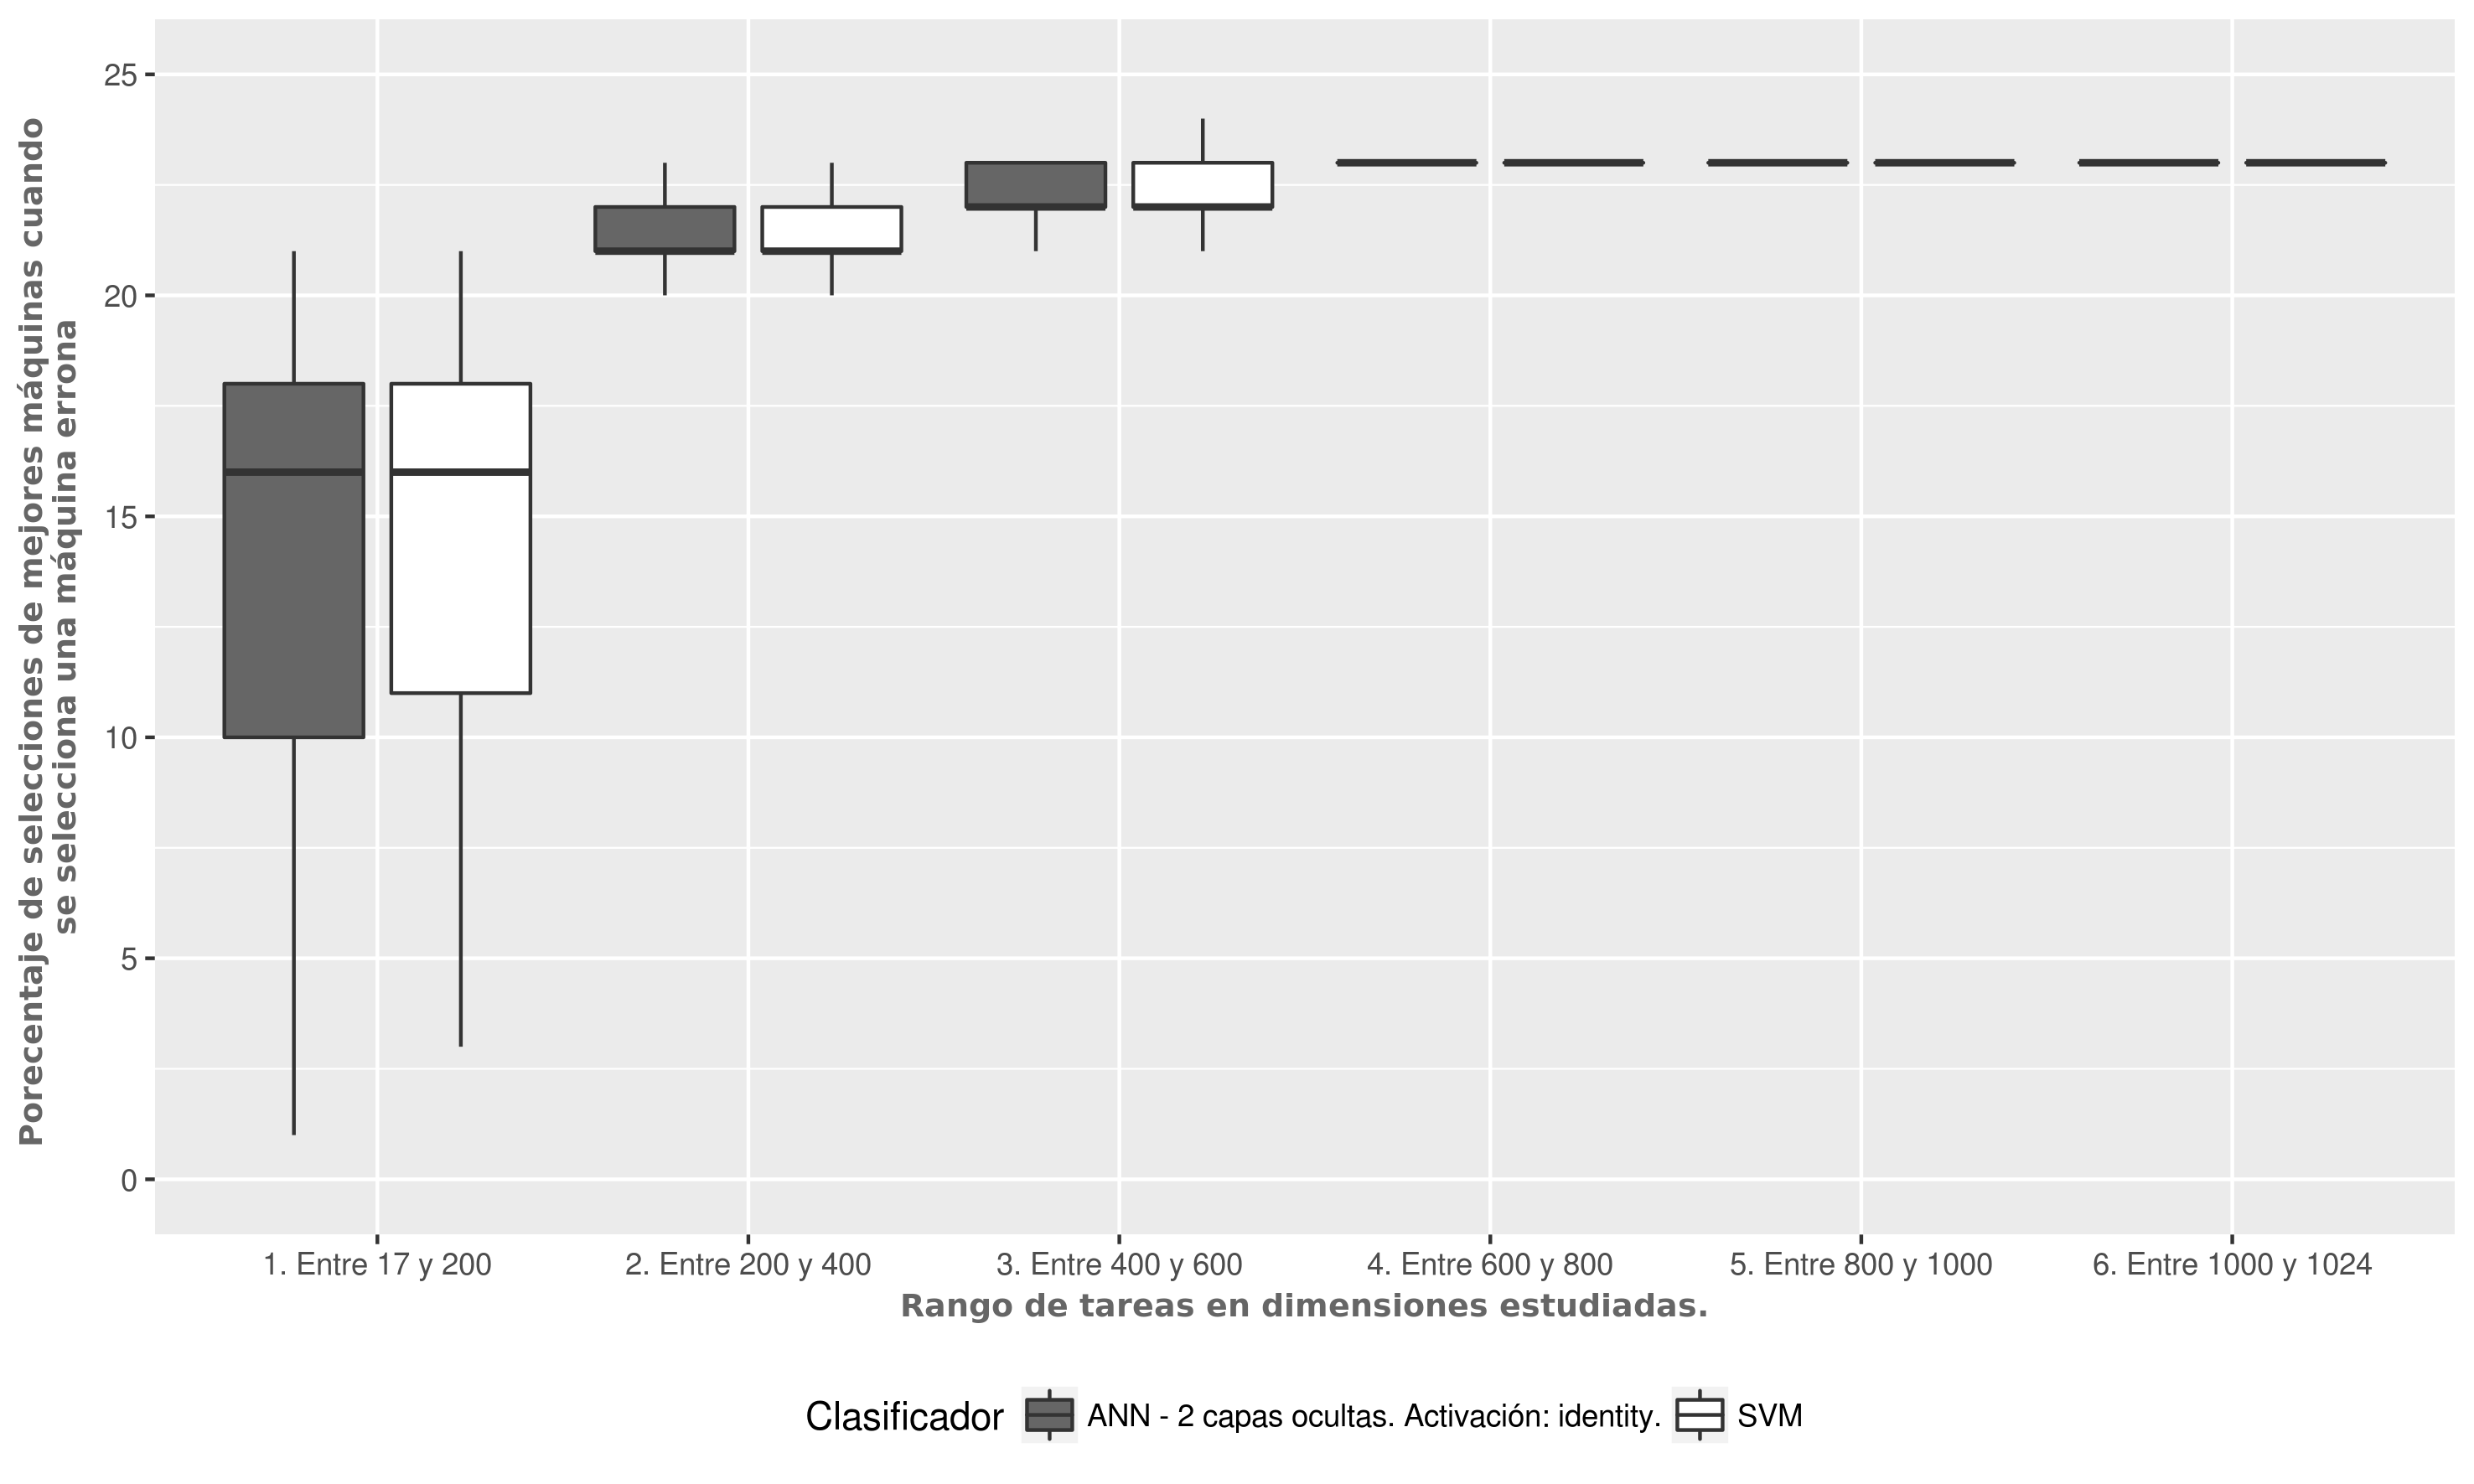
\includegraphics[width=\columnwidth]{imagenes/identity/4_porcentaje_maquinas_mejores_ann_2_capas_ocultas_identity.png}
  \caption{Porcentaje de selección de máquinas mejores frente a una selección diferente a la esperada para la red neuronal con activación \textit{identity} de dos capas ocultas y para la SVM.}
  \label{fig:identity_mejores}
\end{figure}

\newpage % orphaned line.

\section{Red neuronal con activación \textit{tanh} de dos capas ocultas}

La Figura \ref{fig:tanh_makespan} muestra las diferencias porcentuales de \textit{makespan} para la red neuronal con activación \textit{tanh} y para la SVM.
En esta se observa una leve mejora en \textit{makespan} para la red neuronal con respecto al \textit{makespan} obtenido con SVM, para dimensiones grandes.
Esta mejora va acompañada de una mejora en la precisión, sustancial en comparación con las precisiones de las otras funciones de activación estudiadas, como se observa en la Figura \ref{fig:tanh_accuracy}.

\begin{figure}[H]
  \centering
  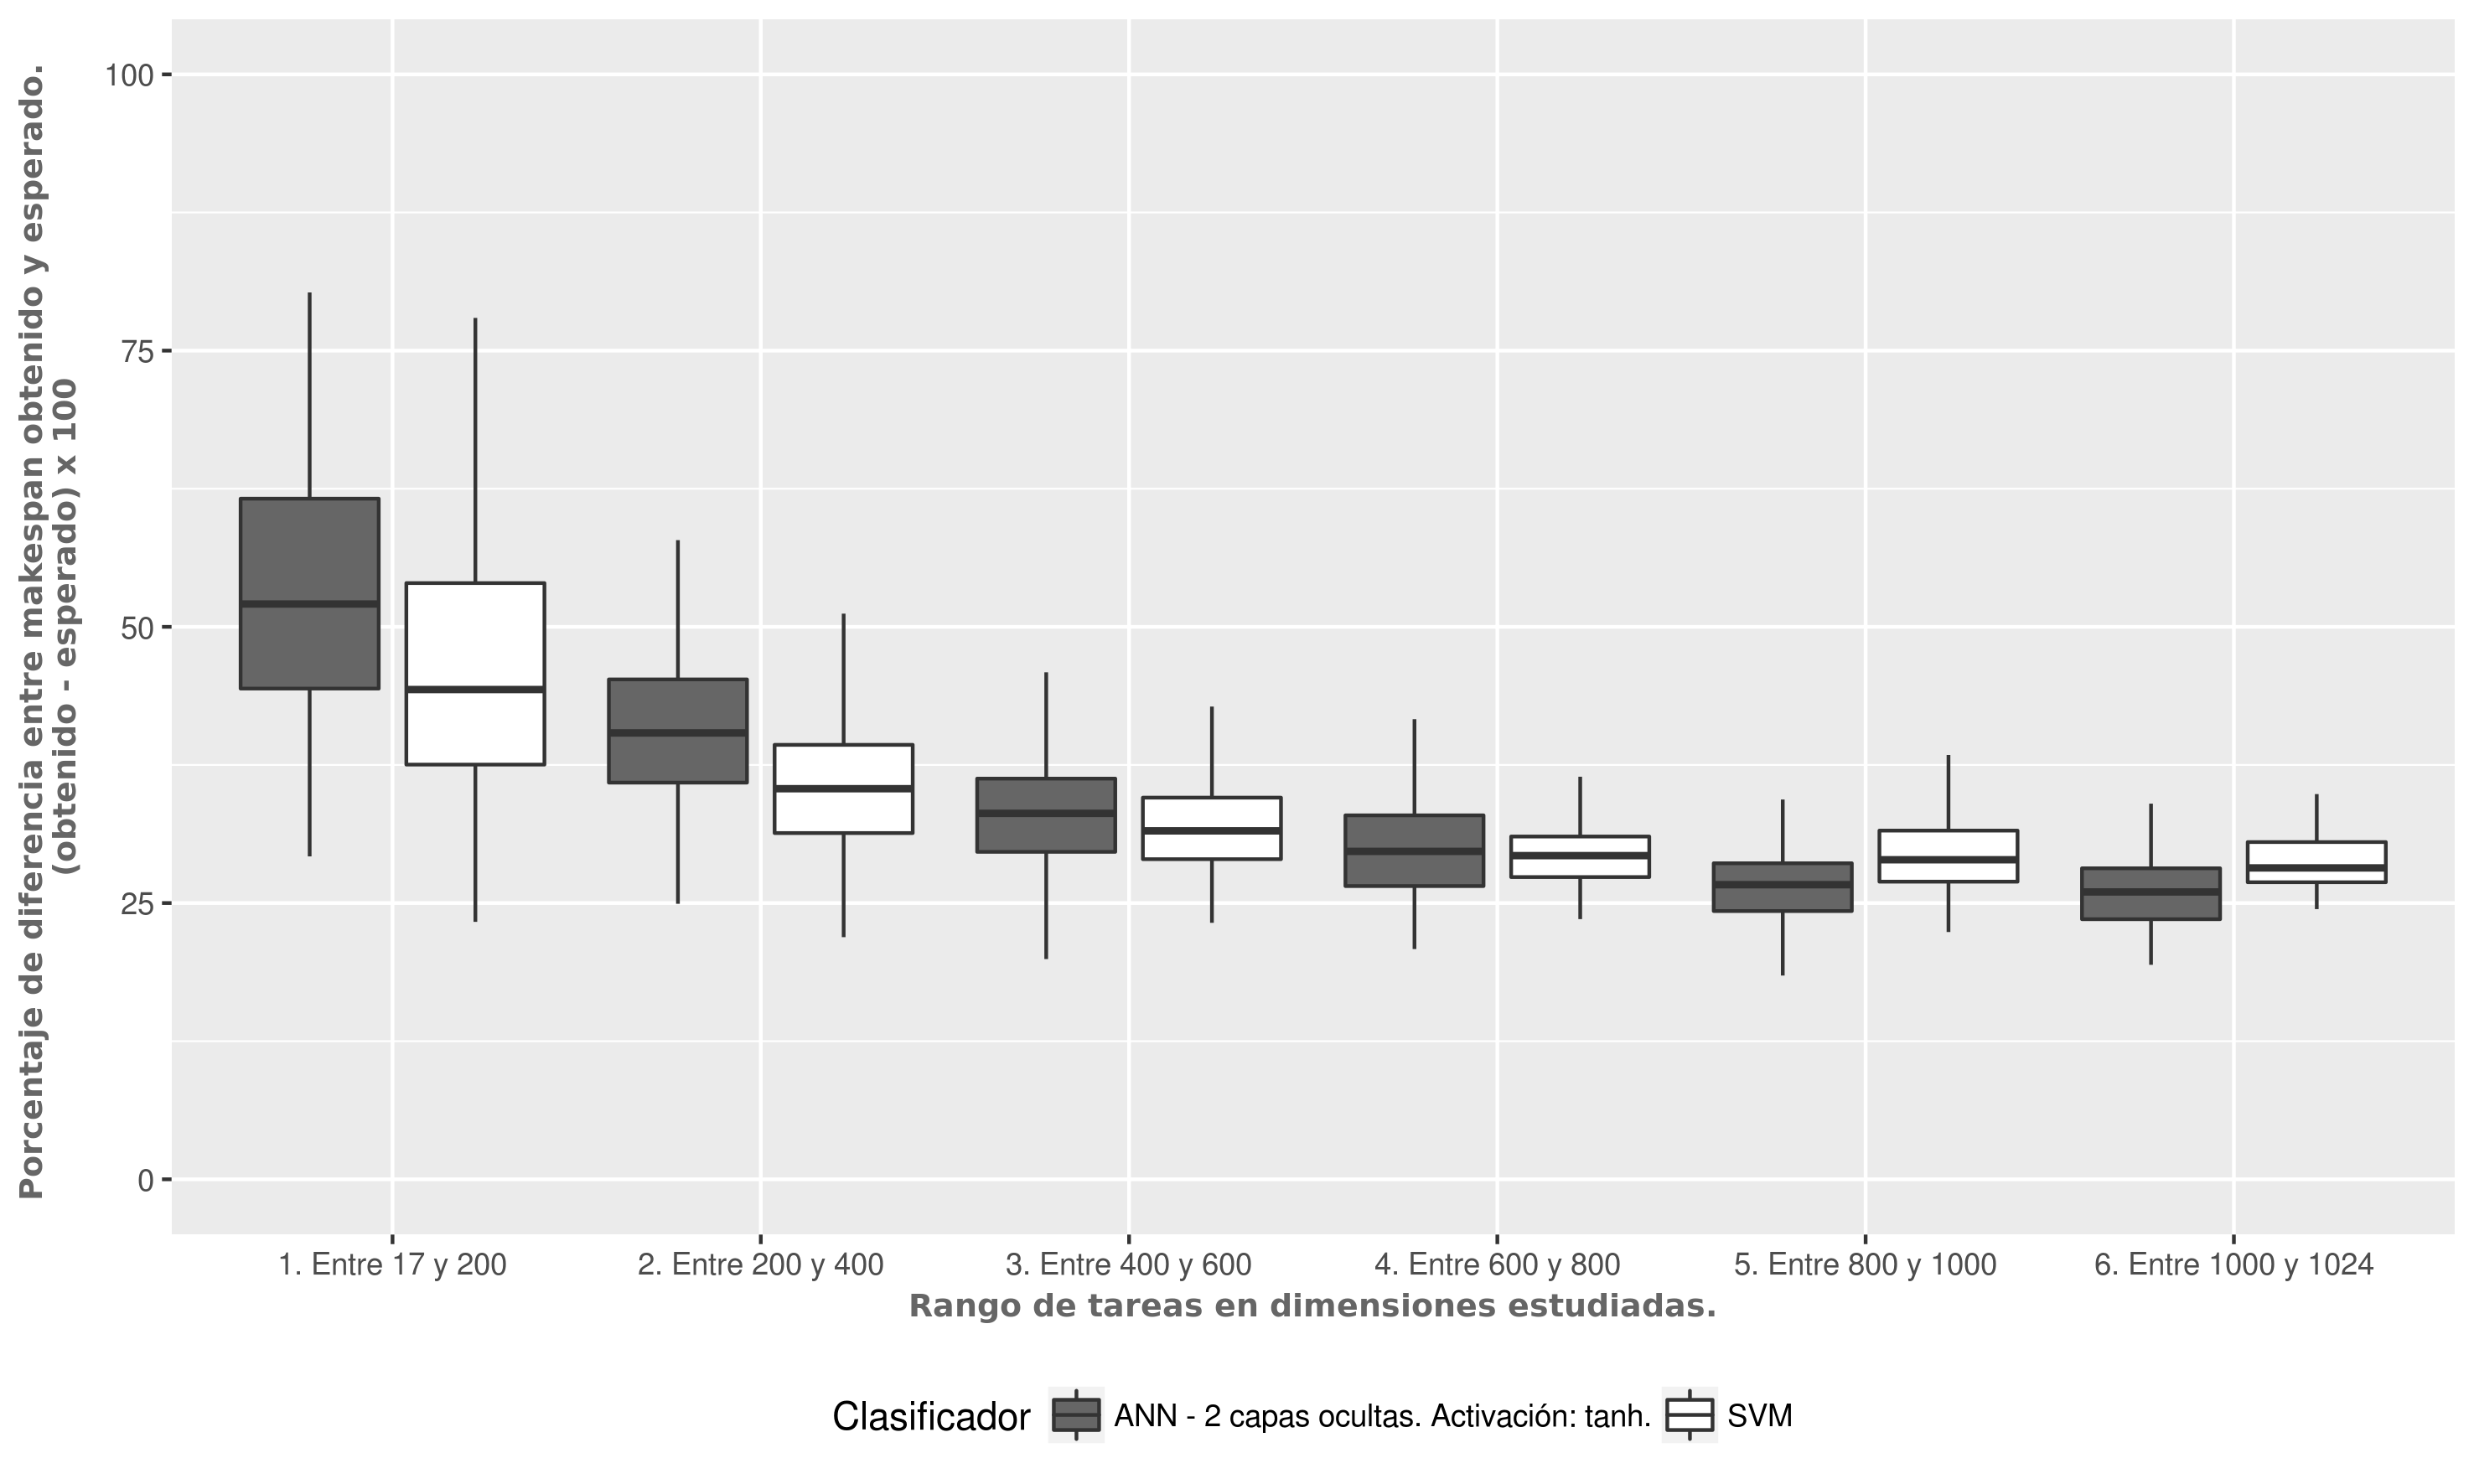
\includegraphics[width=\columnwidth]{imagenes/tanh/2_medianas_diferenciasann_2_capas_ocultas_tanh.png}
  \caption{Comparación de la diferencia porcentual de \textit{makespan} para la red neuronal con activación \textit{tanh}, de dos capas ocultas con respecto a los valores esperados obtenidos con el algoritmo Min-Min.
Así también se muestran los resultados obtenidos para la SVM.
Los resultados se muestran divididos en rangos de dimensión desde $ 17 \times 16$ a $ 1024 \times 16$}
  \label{fig:tanh_makespan}
\end{figure}

\newpage % orphaned line.

\begin{figure}[H]
  \centering
  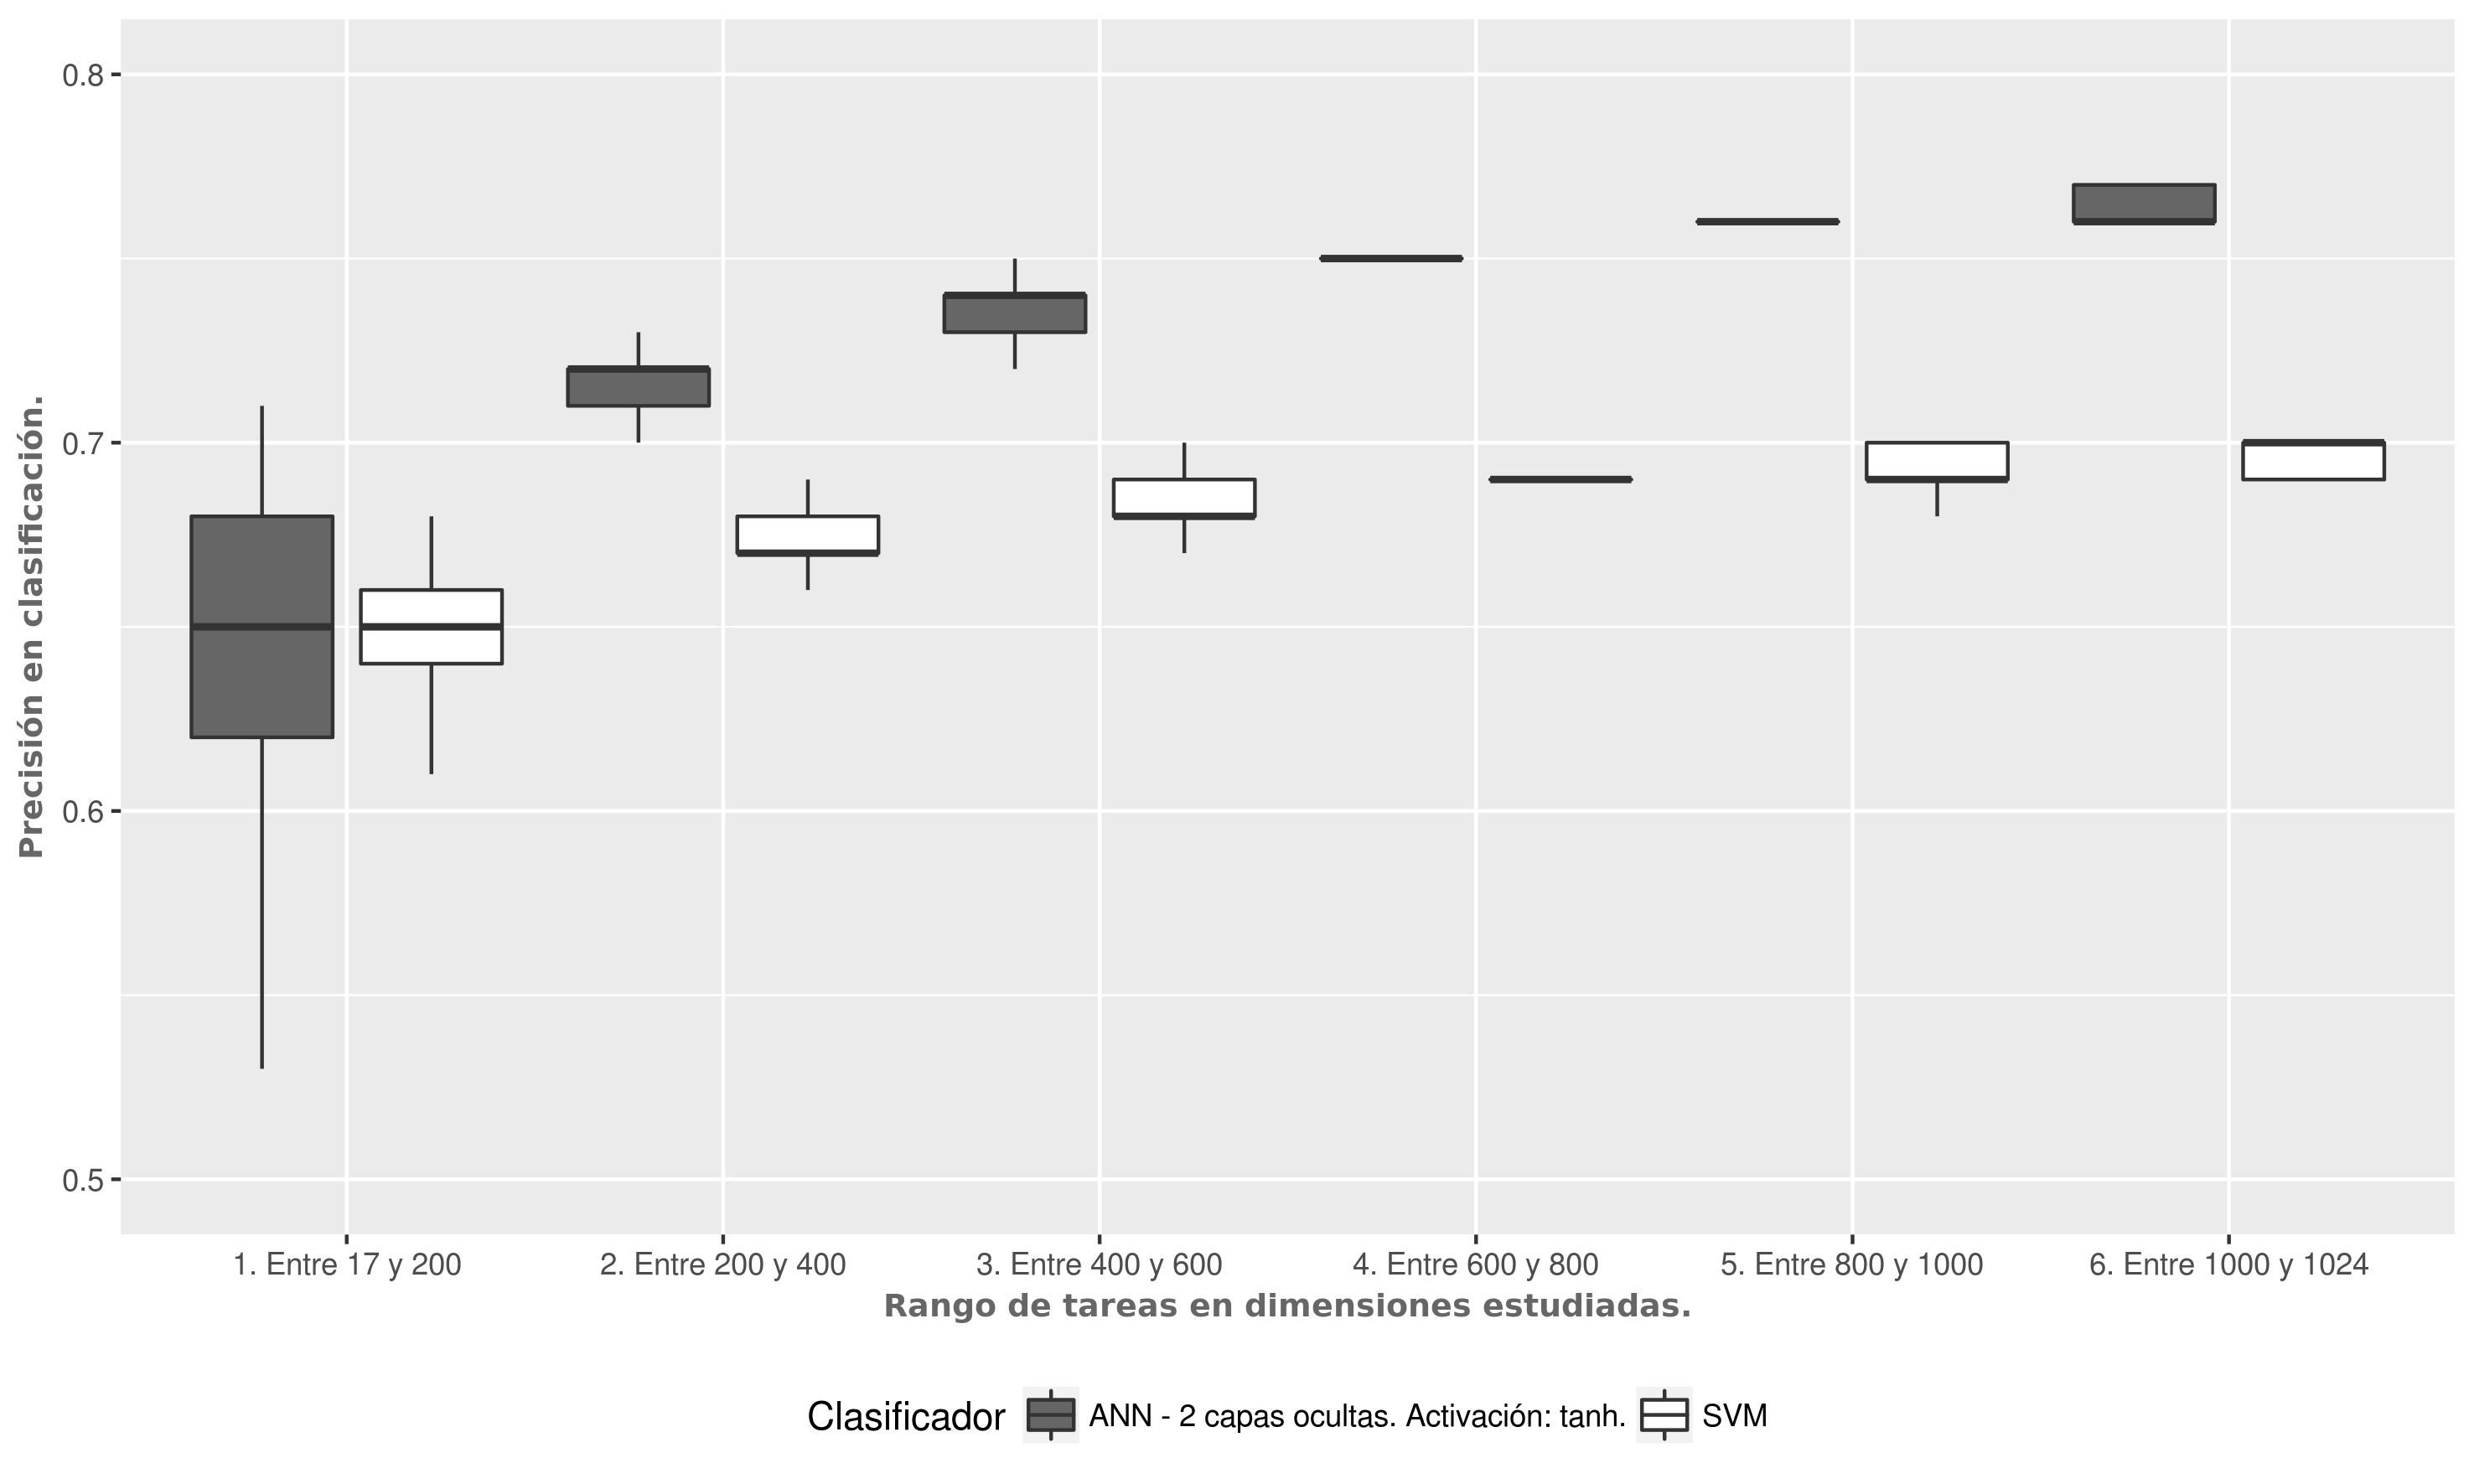
\includegraphics[width=\columnwidth]{imagenes/tanh/3_accuracy_ann_2_capas_ocultas_tanh.png}
  \caption{Precisión en clasificación para la red neuronal con función de activación \textit{tanh} y para la SVM.
Los resultados se muestran divididos en rangos de dimensión desde $ 17 \times 16$ a $ 1024 \times 16$.}
  \label{fig:tanh_accuracy}
\end{figure}

\paragraph{} La Figura \ref{fig:tanh_mejores} muestra que la red neuronal con función de activación \textit{tanh} selecciona máquinas más lentas que SVM cuando se selecciona una máquina diferente a la esperada.

\paragraph{} Para dimensiones grandes se selecciona alrededor de un $15\%$ de mejores máquinas para la función de activación \textit{tanh}, siendo este porcentaje el más bajo obtenido para todas las funciones de activación estudiadas.
Esto conduce a pensar que la precisión es fundamental para aproximarse al \textit{makespan} esperado y que las decisiones que se toman a la hora de seleccionar una máquina diferente a la esperada pierde importancia frente a una precisión elevada en clasificación, donde un error puede costar caro en términos de tiempos de ejecución o \textit{makespan}.

\newpage % orphaned line.

\begin{figure}[H]
  \centering
  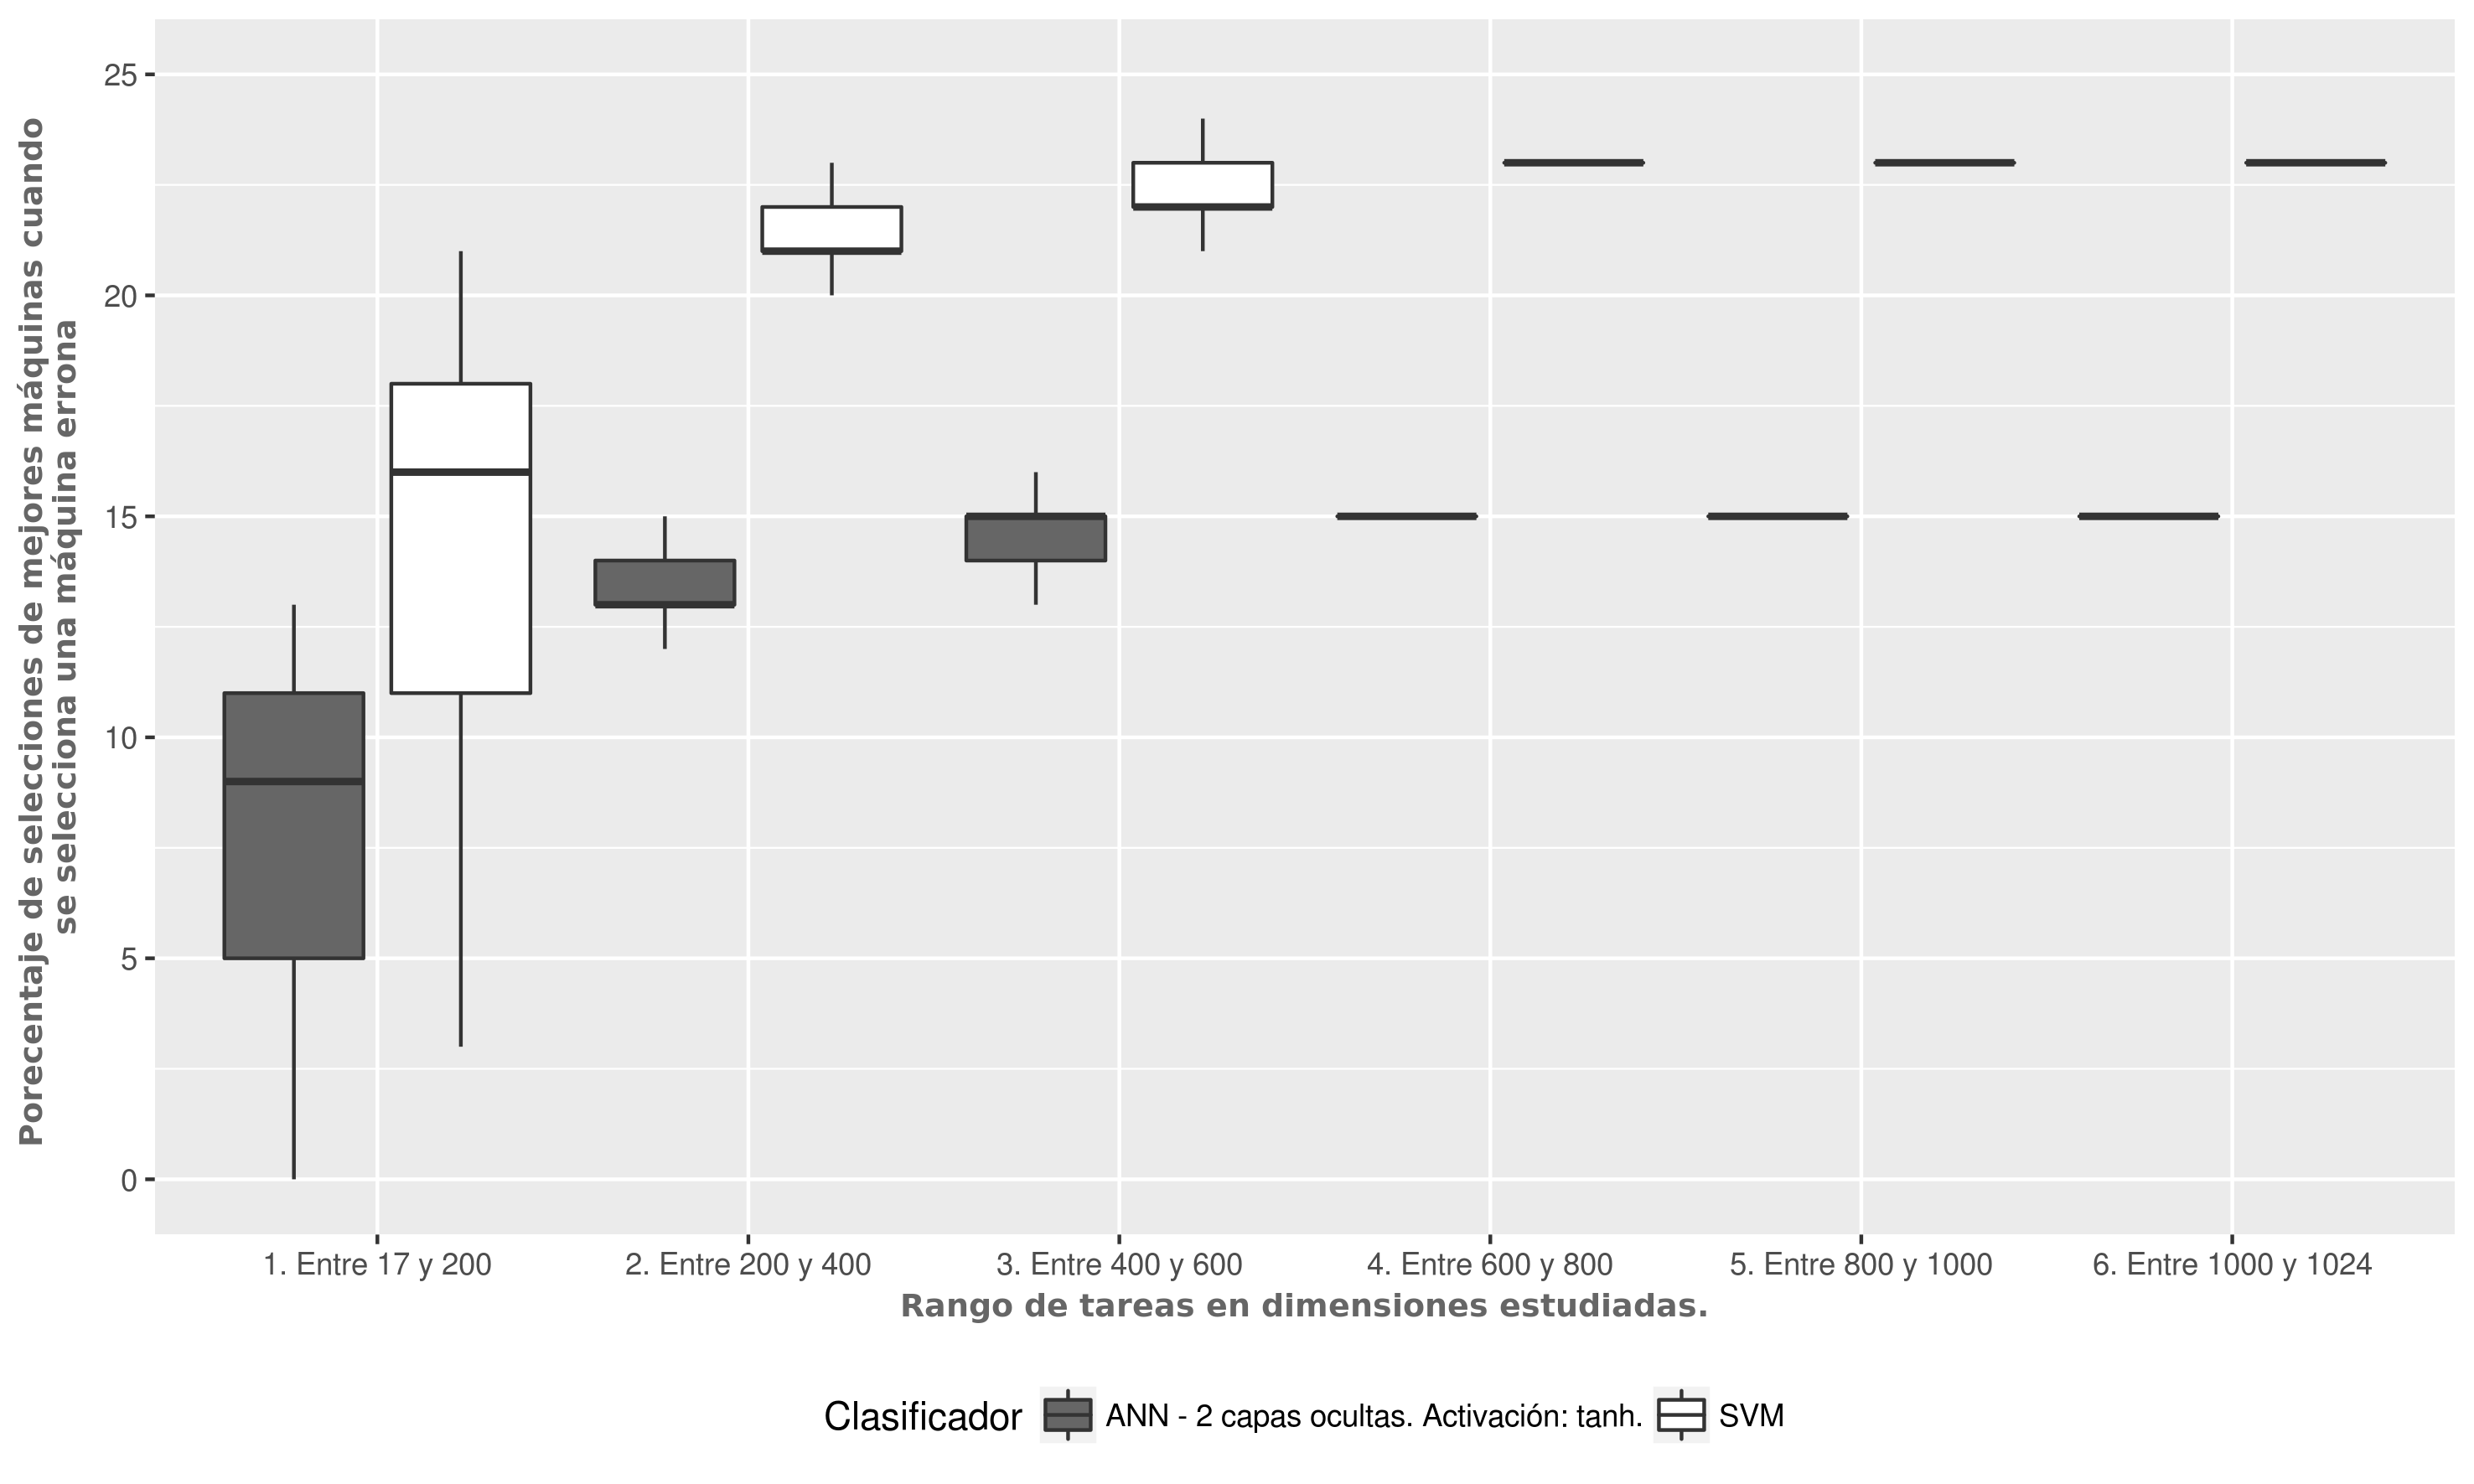
\includegraphics[width=\columnwidth]{imagenes/tanh/4_porcentaje_maquinas_mejores_ann_2_capas_ocultas_tanh.png}
  \caption{Porcentaje de selección de máquinas mejores frente a una selección diferente a la esperada para la red neuronal con activación \textit{tanh} de dos capas ocultas y para la SVM.}
  \label{fig:tanh_mejores}
\end{figure}

\newpage % orphaned line.

\section{Observaciones generales}

\paragraph{} En términos generales, entrenar redes neuronales con menor cantidad de capas ocultas, generó mejores resultados de \textit{makespan} en clasificación, que entrenar redes neuronales con mayor cantidad de capas ocultas.
Esto se traduce en mejores resultados de \textit{makespan} con una menor inversión en tiempo de entrenamiento. 

\paragraph{} Para redes neuronales entrenadas utilizando \textit{tanh} e \textit{identity} como funciones de activación, el \textit{makespan} de los resultados mejoró levemente con respecto al \textit{makespan} de los resultados obtenidos con SVM para dimensiones grandes del problema.
Se observó una relación directa entre la precisión y la mejora porcentual de \textit{makespan} para la red neuronal con activación \textit{tanh}. También se observó una relación entre el porcentaje de selección de mejores máquinas frente a un error y la mejora porcentual de \textit{makespan}, donde una buena selección de máquina frente a un error en la clasificación, puede mitigar los efectos negativos sobre el \textit{makespan} que genera tener una precisión baja. La red neuronal de dos capas ocultas con función de activación \textit{tanh} obtuvo resultados similares en cuanto a \textit{makespan} que la red neuronal de dos capas ocultas con función de activación \textit{identity}, pero la primera obtuvo mejores valores de precisión en clasificación, lo cual hace de la red neuronal con activación \textit{tanh} una configuración de red neuronal potencialmente adecuada para aprender a resolver el problema HCSP.

\paragraph{} Los resultados obtenidos con la red neuronal con función de activación \textit{relu} no mejoraron los resultados obtenidos con SVM en términos de \textit{makespan}, obteniendo precisiones en clasificación similares, teniendo un porcentaje menor de selección de mejores máquinas frente a un error. Esto hace que \textit{relu} sea una función de activación poco adecuada si el objetivo perseguido es aprender a resolver el problema HCSP.
  \chapter{Conclusiones y trabajo futuro} \label{section-conclusiones}
\markright{Conclusiones}

\paragraph{}En este capítulo se presentan las conclusiones del trabajo realizado en este proyecto de grado y las principales líneas de trabajo futuro.

\section{Conclusiones}

\paragraph{}En este proyecto se presentó un estudio comparativo entre dos tipos de clasificadores de aprendizaje automático, SVM y redes neuronales, en el contexto de aprender a resolver el problema \textit{HCSP}, bajo el paradigma Savant Virtual.
Se entrenaron diferentes configuraciones de redes neuronales y de SVM, y se compararon las soluciones obtenidas por cada uno de los clasificadores en términos de su \textit{makespan}, precisión y decisiones de selección de máquinas frente a asignaciones erróneas.
Las redes neuronales fueron entrenadas utilizando distintas funciones de activación, así como también variando la cantidad de capas ocultas, manteniendo los demás parámetros de configuración constantes.
De esta manera, se generaron 9 redes neuronales de 2, 3 y 4 capas ocultas para las funciones de activación \textit{tanh}, \textit{relu} e \textit{identity} respectivamente.
Fueron utilizadas para el entrenamiento 100 instancias del problema de 512 tareas y 16 máquinas, lo que se traduce en 51200 instancias de entrenamiento.
Se profundizó el estudio para aquellas redes neuronales que mostraron mejores resultados en cuanto al \textit{makespan} obtenido.

\paragraph{}El análisis experimental fue realizado clasificando instancias del problema de diferentes dimensiones, desde 17 tareas y 16 máquinas hasta 1024 tareas y 16 máquinas, con el fin de analizar el comportamiento de los clasificadores para instancias más pequeñas, de igual y mayor tamaño en comparación a los datos utilizados durante el entrenamiento, de 512 tareas y 16 máquinas.
Para cada dimensión del problema se utilizaron 10 instancias del problema como instancias de validación y se calculó el \textit{makespan} obtenido mediante la clasificación con las redes neuronales y SVM, así como la precisión y el porcentaje de selección de máquinas más rápidas frente a un error para el promedio de las 10 instancias del problema.

\paragraph{}Los resultados experimentales muestran que las redes neuronales de 2 capas ocultas generaron soluciones con un menor \textit{makespan} que aquellas con 3 y 4 capas ocultas; esto es una característica común a todas las redes neuronales utilizadas sin importar su función de activación.
Además, el \textit{makespan} tiende a ser menos variable para estas redes neuronales, lo cual es de importancia dado que el \textit{makespan} se entiende como la métrica fundamental del éxito de una solución generada para el problema.

\paragraph{}En comparación con SVM, las redes neuronales de dos capas ocultas con funciones de activación \textit{tanh} e \textit{identity} mostraron mejoras en \textit{makespan} para dimensiones grandes.
Para dimensiones a partir de 400 tareas y 16 máquinas se comenzó a observar mejoras en el \textit{makespan} para los resultados obtenidos con ambas redes neuronales.
En particular, la red neuronal de 2 capas ocultas con activación \textit{tanh}, mejoró el \textit{makespan} para dimensiones grandes, teniendo una mejor precisión en clasificación que SVM y teniendo un porcentaje de selección más bajo de máquinas más rápidas frente a errores que SVM.
En cuanto a la red neuronal de dos capas ocultas con función de activación \textit{identity} se observa que la precisión en clasificación es muy similar a la precisión en clasificación de SVM, con menos variabilidad. El porcentaje de selección de máquinas más rápidas para la red neuronal con activación \textit{identity} también presentó poca variabilidad, también mostrando leves mejoras en el \textit{makespan} de las soluciones.
Para las redes neuronales de dos capas ocultas entrenadas con la función de activación \textit{relu} los resultados en cuanto a \textit{makespan} no mejoraron el \textit{makespan} obtenido por SVM. Para las redes neuronales con activación \textit{relu}, la precisión en clasificación resultó levemente mayor que la precisión en clasificación de SVM, teniendo un porcentaje de selección de mejores máquinas frente a un error menor que el de SVM.

\paragraph{}En este trabajo se extendió el trabajo original de SV, se probaron nuevos clasificadores y se mejoraron los resultados.

\section{Trabajo futuro}

\paragraph{}A continuación se detallan las principales líneas de trabajo futuro que surgen a raíz del trabajo realizado para este proyecto de grado.

\paragraph{}Las instancias del problema \textit{HCSP} utilizadas para el entrenamiento y prueba de los clasificadores tienen como característica una baja heterogeneidad de tareas y de máquinas. En instancias reales del problema, lo habitual es tener tareas heterogéneas ejecutando en máquinas de características homogéneas o heterogéneas.
Por este motivo, una de las principales líneas de trabajo futuro consiste en entrenar y evaluar clasificadores utilizando instancias del problema de mayor heterogeneidad en tareas y máquinas.
Este estudio permitiría analizar si el comportamiento de aquellas configuraciones de redes neuronales que durante este trabajo mostraron resultados más prometedores es generalizable a instancias reales del problema.
También es de interés probar distintas configuraciones de hiperparámetros de las redes neuronales, ya que durante este trabajo se analizaron redes neuronales entrenadas con diferentes arquitecturas y funciones de activación, dejando el resto de los parámetros de configuración con sus valores predeterminados. Además, es de interés realizar pruebas con otros clasificadores de aprendizaje automático realizando estudios comparativos con los resultados ya obtenidos.

\paragraph{}Finalmente, se considera necesario extender este estudio comparativo aplicando búsquedas locales tanto a las soluciones generadas con redes neuronales como a aquellas generadas por SVM, para evaluar el efecto que esto pudiera tener en la calidad de las mismas, ya sea en el marco de una implementación de MapReduce o no, siendo esta la propuesta fundamental del paradigma SV.

% TODO discutir, tema sensible -> Un ejemplo de problema real sobre el cual se puede probar el enfoque es el problema de asignación de contenedores de basura en una ciudad para la optimización de las rutas de los camiones que se encargan de vaciar y mantener los contenedores.

  
  \backmatter % Comando que generalos apéndices, anexos y bibliografía. NO COMENTAR
  
  \bibliography{bibliografia/bibliography} % Agregar la cantidad de archivos .bib que se tengan para la bibliografía.
  \bibend % No comentar
  % 
  % \glosario 		         % Glosario, NO comentar
  %
  % \apenarabicnumbering
  % \apenmatter				 % Apéndices, NO comentar
  % \chapter{Datos procesados}


  % \chapter{Imágenes remasterizadas}\label{Ape2}

  % \chapter{Entrevistas desgrabadas}\label{Ape3}

  % Seguir copiando la linea de arriba para agregar más apéndices.
  %
  % \anexarabicnumbering
  % \anexmatter				 % Anexos, NO comentar
  % \chapter{Material legislativo}\label{Ane1}

XXXXX
  % Seguir copiando la linea de arriba para agregar más anexos.
  % 
\end{document}

% ===== FIN DEL DOCUMENTO =====